\documentclass[11pt, proquest]{uwthesis}[2016/11/22]

\usepackage{amsmath}
\usepackage{setspace}
\usepackage{mathpartir}
\usepackage[usenames,dvipsnames]{color}
\usepackage{alltt}
\usepackage{textcomp}
\usepackage{amscd}
\usepackage{amsfonts}
\usepackage{varwidth}
\usepackage{listings}
\usepackage{float}
\usepackage[noend]{algorithmic}
\usepackage{mathrsfs}
\usepackage{stmaryrd}
\usepackage{verbatim}
\usepackage{lipsum}
\usepackage{wrapfig}
\newcounter{tags}
\usepackage{enumitem}
\usepackage{fancyvrb}
\fvset{fontsize=\scriptsize}
\renewcommand{\ttdefault}{txtt} % provide bold tt in alltt

%\usepackage{libertine}
\usepackage[T1]{fontenc}

\usepackage[numbers]{natbib}

\usepackage{graphicx}
\usepackage{pifont}
\usepackage{xspace}
\usepackage{url}
\usepackage{relsize}
\usepackage[colorlinks=true,allcolors=black,breaklinks,draft=false]{hyperref}
\usepackage{amssymb}
\usepackage{amsthm}
\theoremstyle{definition}
\newtheorem{theorem}{Theorem}
\newtheorem{definition}{Definition}[section]
\newtheorem{lemma}[theorem]{Lemma}
\newtheorem{proposition}[theorem]{Proposition}
\newtheorem{corollary}[theorem]{Corollary}



\usepackage[capitalise]{cleveref}
\Crefname{thm}{Theorem}{Theorems}

\usepackage{tikz}
\usetikzlibrary{calc}
\usetikzlibrary{shapes.callouts}

\usepackage{multirow}
\usepackage{booktabs}

\setcounter{tocdepth}{1}

% :)
\def\pgascse{Paul G. Allen School of Computer Science \& Engineering}

% Latin abbreviations
%   https://www.e-education.psu.edu/styleforstudents/c3_p28.html
%   http://public.wsu.edu/~brians/errors/e.g.html
\newcommand{\etal}{et~al.\xspace}
\newcommand{\ie}{i.e.\xspace}
\newcommand{\eg}{e.g.\xspace}
\newcommand{\etc}{etc.\xspace}

\newcommand{\mypyvy}{\texttt{mypyvy}\xspace}

% \newcommand{\todo}[1]{\relax}
\newcommand{\todo}[1]{{\color{red}\bfseries [[#1]]}}


\begin{document}

\prelimpages

\Title{Compositional and Automated Verification of Distributed Systems}
\Author{James R. Wilcox}
\Year{2019}
\Program{\pgascse}

% \Chair{Zachary Tatlock}{Professor}{\pgascse}
% \Signature{Dan Grossman}
% \Signature{Thomas Anderson}

\titlepage

\copyrightpage

\setcounter{page}{-1} \abstract{%
  Distributed systems provide the backbone for modern computer
  systems, from cloud computing to air-traffic control.  These complex
  systems execute concurrently in unreliable environments and are
  expected to tolerate various faults.  Such environments are
  notoriously difficult to adequately model with testing, but because
  of the critical importance of these systems, it is essential that
  they are correct.  It thus makes sense to turn to more rigorous
  methods of ensuring correctness, such as formal verification.
  Applying formal methods is not a panacea, however, due to the
  complexity of the systems involved.  It is not uncommon, \eg, for a
  distributed file system to coordinate thousands of machines using a
  combination of several different protocols to ensure consistency,
  fault tolerance, and high performance.  In order to verify such a
  system, one must break the problem down into smaller parts, each of
  which is individually verifiable, ideally with a high degree of
  automation.

  This dissertation describes programming languages techniques for
  doing just that, namely, for verifying distributed systems
  compositionally and automatically.  First, we present Verdi, a
  framework for verifying distributed systems in the Coq proof
  assistant, which allows reasoning about fault tolerance mechanisms
  as transformers between fault models. Second, we detail Disel, a
  concurrent separation logic for distributed systems whose key
  insight is to treat the network as analogous to the heap in
  sequential programming.  Finally, we report on mypyvy, a
  domain-specific language for describing symbolic transition systems
  in first-order logic, which supports a variety of automated
  reasoning tools to analyze systems.
}

\tableofcontents
%\listoffigures
%\listoftables  % I have no tables

\acknowledgments{% \vskip2pc
  % {\narrower\noindent
  Acks.
  % \par}
}

%\dedication{\begin{center}dedication\end{center}}

\textpages

\chapter{Introduction}
\label{chap:intro}

\begin{verbatim}
New intro outline:
- Barkley :D
- distributed systems
  - pervasive
  - critical
  - fail often
  - hard to get right
- fail often + hard to get right because:
  - concurrency
  - forced locality (data is distributed!)
  - failure
  - the combination of forced locality and failure -> partial failure
    - ie, cannot observe globally who has definitely failed vs not
- very difficult to test thoroughly
  - interleavings of concurrent actions
  - whether and when certain failures occur
  - not to mention the usual testing difficulties for sequential programs
    - data coverage, etc
- primary challenge: system/proof complexity
- solution: system/proof compositionality
- thesis: PL techniques for compositionality lay the foundations for effective
  verification of distributed systems implementations.
- remainder of thesis in three parts
  - challenge 1: fault tolerance
    solution 1: VSTs to decompose tolerance from app
  - challenge 2: many components
    solution 2: separation logic with composition theorem
  - challenge 3: proof effort
    solution 3: proof automation that takes advantage of small components to
                bring decidability/high automation
\end{verbatim}

Distributed systems are widely used
  in everything from web infrastructure to airplanes,
  and their correctness is critical.
These systems are notoriously hard to implement correctly
  because they execute
  across multiple nodes in unreliable environments
  and are expected to tolerate various faults.
Traditional testing techniques are insufficient
  to adequately explore the space of possible executions
  in the presence of concurrency and failure,
  because such tests would have to enumerate
  all interleavings of system events and failure events
  in a simulation of the system.
In response to this challenge,
  formal methods have been applied
  to exhaustively check correctness of distributed systems,
  but most such techniques work only on \emph{models} of the system,
  which results in a formality gap between the model and its implementation.
For example, classical model checking
  has been shown to be extremely effective
  in finding concurrency and fault-tolerance bugs at the design level,
  but it does not scale to the complex data structures used in real systems.
Formal verification
  using human-guided, automated, machine-checked proofs
  is the only technique that can provide the desired guarantees for such systems.

Applying formal methods is not a panacea, however, due to the
complexity of the systems involved.  It is not uncommon, \eg, for a
distributed file system to coordinate thousands of machines using a
combination of several different protocols to ensure consistency,
fault tolerance, and high performance.  To verify such a
system, one must break the problem down into smaller parts.
This decomposition yields benefits of automation in two senses.
First, a truly compositional proof imposes no additional proof
burden to put the pieces back together. Second, sufficiently
decomposed pieces can be reasoned about fully automatically
using decision procedures. 

The central claim of this dissertation is:
\begin{center}
\emph{Programming languages techniques for compositionality
  lay the foundations for effective, automated verification of
  distributed systems implementations.
}
\end{center}

\Cref{chap:verdi} presents Verdi, a Coq-based framework for implementing and
verifying distributed systems.  Verdi models the system execution
using various \emph{network semantics}, each of which encodes
assumptions about the environment including possible network faults
and machine failures.  Network semantics can range from the idealistic
to the pessimistic. For example, one might assume that all messages
are eventually delivered and that nodes never fail. On the other hand,
one might assume that packets can be dropped and duplicated and that
some nodes behave arbitrarily or maliciously. Different systems are
designed under different sets of assumptions, and network semantics
capture those assumptions.
The main point of defining a particular network semantics in Verdi is to verify
distributed systems using that semantics as the fault model.
Assuming the network semantics
accurately describes all possible behaviors of the system's
environment, Verdi guarantees that the system is correct for all executions.
For common network semantics, there are typically generic mechanisms
that systems use to tolerate faults, \eg sequence numbering to handle
message reordering and duplication. Another key benefit of clearly
stating environment assumptions as network semantics is that one
can then express these generic fault tolerance mechanisms as \emph{transformers}
between semantics.
Using transformers, the engineer can implement and reason about their
application in a fault model
with relatively few faults, and then automatically transform the system
into one that provably works in a more adversarial fault model with
relatively more faults. 

%whose key insight is to treat the network as analogous to the heap in
%sequential programming.


\Cref{chap:disel} details Disel, a concurrent separation logic for distributed
systems.  Whereas Verdi separates fault tolerance reasoning from
application logic (which we call vertical compositionality), Disel
separates reasoning about cooperating services by defining interfaces
that capture protocol-specific invariants (which we call horizontal
compositionality).  This supports verifying modern distributed systems
which are typically built by composing several services to provide a
high-level application.  A proof of correctness for a system composed
of several services should similarly compose the guarantees of each
individual service. Using the techniques of Verdi alone, such reasoning
is not possible. Instead of needing to reason across fault models,
what we need is the ability to abstract over the low-level details
provides its guarantee. To achieve this, we take inspiration from
modern program logics for concurrent programs that manipulate
heap pointers. These logics allow modular reasoning by separating
different parts of the heap, each of which can be reasoned about
independently. Disel applies this insight to distributed systems
by analogizing the network as the heap. Thus, Disel separates
the network messages of each protocol from each other, allowing
independent reasoning. Disel achieves this through several
novel logical mechanisms that support strengthening the invariants
of other services with client-specific facts and capturing the
essential interactions between protocols with \emph{hooks}, which
allow one protocol's actions to be conditioned on another protocol's
state.

Experience in Disel and Verdi showed that the manual effort required
to provide strong guarantees about distributed systems doesn't scale
with current tooling.  In particular, the key sticking point is
developing inductive invariants.  Deductive verification techniques,
such as those used in Disel and Verdi, are highly expressive but
require the user to provide a great deal of additional input,
including inductive invariants and their proofs. For example, using
Verdi to prove an application correct in a relatively nice fault model
still requires deriving an application-specific invariant, which
simultaneously (1) summarizes all the reachable states of the
application, (2) is closed under the transition system's step
relation, and (3) ensures the absence of safety violations.
The difficulty of deriving these invariants inspired us to
investigate techniques for proving and even \emph{inferring}
inductive invariants automatically.

\Cref{chap:mypyvy} describes \mypyvy, a tool for automated reasoning about
symbolic transition systems in first-order logic and supports a
variety of automated reasoning tools to analyze systems.
\mypyvy takes an input file describing a symbolic transition system
and performs the analysis requested by the user. Three of the most
interesting analyses include inductive invariant checking,
invariant inference, and bounded trace reasoning.
In all cases, \mypyvy loads the transition system and compiles
it together with the user-requested analysis to a (sequence of) SMT queries,
which are dispatched by Z3.

Distributed systems remains a crucial topic with many potential avenues
for future work. In \cref{chap:conclusion}, we summarize our plans for extending
Verdi, Disel, and \mypyvy to further improve the verification experience.
We are especially excited to live in a world where more users are
empowered to verify their distributed systems.
\chapter{Verdi}
\label{chap:verdi}


\makeatletter
\def\PY@reset{\let\PY@it=\relax \let\PY@bf=\relax%
    \let\PY@ul=\relax \let\PY@tc=\relax%
    \let\PY@bc=\relax \let\PY@ff=\relax}
\def\PY@tok#1{\csname PY@tok@#1\endcsname}
\def\PY@toks#1+{\ifx\relax#1\empty\else%
    \PY@tok{#1}\expandafter\PY@toks\fi}
\def\PY@do#1{\PY@bc{\PY@tc{\PY@ul{%
    \PY@it{\PY@bf{\PY@ff{#1}}}}}}}
\def\PY#1#2{\PY@reset\PY@toks#1+\relax+\PY@do{#2}}

\expandafter\def\csname PY@tok@gd\endcsname{\def\PY@tc##1{\textcolor[rgb]{0.63,0.00,0.00}{##1}}}
\expandafter\def\csname PY@tok@gu\endcsname{\let\PY@bf=\textbf\def\PY@tc##1{\textcolor[rgb]{0.50,0.00,0.50}{##1}}}
\expandafter\def\csname PY@tok@gt\endcsname{\def\PY@tc##1{\textcolor[rgb]{0.00,0.27,0.87}{##1}}}
\expandafter\def\csname PY@tok@gs\endcsname{\let\PY@bf=\textbf}
\expandafter\def\csname PY@tok@gr\endcsname{\def\PY@tc##1{\textcolor[rgb]{1.00,0.00,0.00}{##1}}}
\expandafter\def\csname PY@tok@cm\endcsname{\let\PY@it=\textit\def\PY@tc##1{\textcolor[rgb]{0.25,0.50,0.50}{##1}}}
\expandafter\def\csname PY@tok@vg\endcsname{\def\PY@tc##1{\textcolor[rgb]{0.10,0.09,0.49}{##1}}}
\expandafter\def\csname PY@tok@mh\endcsname{\def\PY@tc##1{\textcolor[rgb]{0.40,0.40,0.40}{##1}}}
\expandafter\def\csname PY@tok@go\endcsname{\def\PY@tc##1{\textcolor[rgb]{0.53,0.53,0.53}{##1}}}
\expandafter\def\csname PY@tok@ge\endcsname{\let\PY@it=\textit}
\expandafter\def\csname PY@tok@vc\endcsname{\def\PY@tc##1{\textcolor[rgb]{0.10,0.09,0.49}{##1}}}
\expandafter\def\csname PY@tok@il\endcsname{\def\PY@tc##1{\textcolor[rgb]{0.40,0.40,0.40}{##1}}}
\expandafter\def\csname PY@tok@cs\endcsname{\let\PY@it=\textit\def\PY@tc##1{\textcolor[rgb]{0.25,0.50,0.50}{##1}}}
\expandafter\def\csname PY@tok@cp\endcsname{\def\PY@tc##1{\textcolor[rgb]{0.74,0.48,0.00}{##1}}}
\expandafter\def\csname PY@tok@gi\endcsname{\def\PY@tc##1{\textcolor[rgb]{0.00,0.63,0.00}{##1}}}
\expandafter\def\csname PY@tok@gh\endcsname{\let\PY@bf=\textbf\def\PY@tc##1{\textcolor[rgb]{0.00,0.00,0.50}{##1}}}
\expandafter\def\csname PY@tok@ni\endcsname{\let\PY@bf=\textbf\def\PY@tc##1{\textcolor[rgb]{0.60,0.60,0.60}{##1}}}
\expandafter\def\csname PY@tok@nl\endcsname{\def\PY@tc##1{\textcolor[rgb]{0.63,0.63,0.00}{##1}}}
\expandafter\def\csname PY@tok@nn\endcsname{\let\PY@bf=\textbf\def\PY@tc##1{\textcolor[rgb]{0.00,0.00,1.00}{##1}}}
\expandafter\def\csname PY@tok@no\endcsname{\def\PY@tc##1{\textcolor[rgb]{0.53,0.00,0.00}{##1}}}
\expandafter\def\csname PY@tok@na\endcsname{\def\PY@tc##1{\textcolor[rgb]{0.49,0.56,0.16}{##1}}}
\expandafter\def\csname PY@tok@nb\endcsname{\def\PY@tc##1{\textcolor[rgb]{0.00,0.50,0.00}{##1}}}
\expandafter\def\csname PY@tok@nc\endcsname{\let\PY@bf=\textbf\def\PY@tc##1{\textcolor[rgb]{0.00,0.00,1.00}{##1}}}
\expandafter\def\csname PY@tok@nd\endcsname{\def\PY@tc##1{\textcolor[rgb]{0.67,0.13,1.00}{##1}}}
\expandafter\def\csname PY@tok@ne\endcsname{\let\PY@bf=\textbf\def\PY@tc##1{\textcolor[rgb]{0.82,0.25,0.23}{##1}}}
\expandafter\def\csname PY@tok@nf\endcsname{\def\PY@tc##1{\textcolor[rgb]{0.00,0.00,1.00}{##1}}}
\expandafter\def\csname PY@tok@si\endcsname{\let\PY@bf=\textbf\def\PY@tc##1{\textcolor[rgb]{0.73,0.40,0.53}{##1}}}
\expandafter\def\csname PY@tok@s2\endcsname{\def\PY@tc##1{\textcolor[rgb]{0.73,0.13,0.13}{##1}}}
\expandafter\def\csname PY@tok@vi\endcsname{\def\PY@tc##1{\textcolor[rgb]{0.10,0.09,0.49}{##1}}}
\expandafter\def\csname PY@tok@nt\endcsname{\let\PY@bf=\textbf\def\PY@tc##1{\textcolor[rgb]{0.00,0.50,0.00}{##1}}}
\expandafter\def\csname PY@tok@nv\endcsname{\def\PY@tc##1{\textcolor[rgb]{0.10,0.09,0.49}{##1}}}
\expandafter\def\csname PY@tok@s1\endcsname{\def\PY@tc##1{\textcolor[rgb]{0.73,0.13,0.13}{##1}}}
\expandafter\def\csname PY@tok@sh\endcsname{\def\PY@tc##1{\textcolor[rgb]{0.73,0.13,0.13}{##1}}}
\expandafter\def\csname PY@tok@sc\endcsname{\def\PY@tc##1{\textcolor[rgb]{0.73,0.13,0.13}{##1}}}
\expandafter\def\csname PY@tok@sx\endcsname{\def\PY@tc##1{\textcolor[rgb]{0.00,0.50,0.00}{##1}}}
\expandafter\def\csname PY@tok@bp\endcsname{\def\PY@tc##1{\textcolor[rgb]{0.00,0.50,0.00}{##1}}}
\expandafter\def\csname PY@tok@c1\endcsname{\let\PY@it=\textit\def\PY@tc##1{\textcolor[rgb]{0.25,0.50,0.50}{##1}}}
\expandafter\def\csname PY@tok@kc\endcsname{\let\PY@bf=\textbf\def\PY@tc##1{\textcolor[rgb]{0.00,0.50,0.00}{##1}}}
\expandafter\def\csname PY@tok@c\endcsname{\let\PY@it=\textit\def\PY@tc##1{\textcolor[rgb]{0.25,0.50,0.50}{##1}}}
\expandafter\def\csname PY@tok@mf\endcsname{\def\PY@tc##1{\textcolor[rgb]{0.40,0.40,0.40}{##1}}}
\expandafter\def\csname PY@tok@err\endcsname{\def\PY@bc##1{\setlength{\fboxsep}{0pt}\fcolorbox[rgb]{1.00,0.00,0.00}{1,1,1}{\strut ##1}}}
\expandafter\def\csname PY@tok@kd\endcsname{\let\PY@bf=\textbf\def\PY@tc##1{\textcolor[rgb]{0.00,0.50,0.00}{##1}}}
\expandafter\def\csname PY@tok@ss\endcsname{\def\PY@tc##1{\textcolor[rgb]{0.10,0.09,0.49}{##1}}}
\expandafter\def\csname PY@tok@sr\endcsname{\def\PY@tc##1{\textcolor[rgb]{0.73,0.40,0.53}{##1}}}
\expandafter\def\csname PY@tok@mo\endcsname{\def\PY@tc##1{\textcolor[rgb]{0.40,0.40,0.40}{##1}}}
\expandafter\def\csname PY@tok@kn\endcsname{\let\PY@bf=\textbf\def\PY@tc##1{\textcolor[rgb]{0.00,0.50,0.00}{##1}}}
\expandafter\def\csname PY@tok@gp\endcsname{\let\PY@bf=\textbf\def\PY@tc##1{\textcolor[rgb]{0.00,0.00,0.50}{##1}}}
\expandafter\def\csname PY@tok@kr\endcsname{\let\PY@bf=\textbf\def\PY@tc##1{\textcolor[rgb]{0.00,0.50,0.00}{##1}}}
\expandafter\def\csname PY@tok@s\endcsname{\def\PY@tc##1{\textcolor[rgb]{0.73,0.13,0.13}{##1}}}
\expandafter\def\csname PY@tok@kp\endcsname{\def\PY@tc##1{\textcolor[rgb]{0.00,0.50,0.00}{##1}}}
\expandafter\def\csname PY@tok@w\endcsname{\def\PY@tc##1{\textcolor[rgb]{0.73,0.73,0.73}{##1}}}
\expandafter\def\csname PY@tok@kt\endcsname{\def\PY@tc##1{\textcolor[rgb]{0.69,0.00,0.25}{##1}}}
\expandafter\def\csname PY@tok@ow\endcsname{\let\PY@bf=\textbf\def\PY@tc##1{\textcolor[rgb]{0.67,0.13,1.00}{##1}}}
\expandafter\def\csname PY@tok@sb\endcsname{\def\PY@tc##1{\textcolor[rgb]{0.73,0.13,0.13}{##1}}}
\expandafter\def\csname PY@tok@k\endcsname{\let\PY@bf=\textbf\def\PY@tc##1{\textcolor[rgb]{0.00,0.50,0.00}{##1}}}
\expandafter\def\csname PY@tok@se\endcsname{\let\PY@bf=\textbf\def\PY@tc##1{\textcolor[rgb]{0.73,0.40,0.13}{##1}}}
\expandafter\def\csname PY@tok@sd\endcsname{\let\PY@it=\textit\def\PY@tc##1{\textcolor[rgb]{0.73,0.13,0.13}{##1}}}

\def\PYZbs{\char`\\}
\def\PYZus{\char`\_}
\def\PYZob{\char`\{}
\def\PYZcb{\char`\}}
\def\PYZca{\char`\^}
\def\PYZam{\char`\&}
\def\PYZlt{\char`\<}
\def\PYZgt{\char`\>}
\def\PYZsh{\char`\#}
\def\PYZpc{\char`\%}
\def\PYZdl{\char`\$}
\def\PYZhy{\char`\-}
\def\PYZsq{\char`\'}
\def\PYZdq{\char`\"}
\def\PYZti{\char`\~}
% for compatibility with earlier versions
\def\PYZat{@}
\def\PYZlb{[}
\def\PYZrb{]}
\makeatother



% \|name| or \mathid{name} denotes identifiers and slots in formulas
\def\|#1|{\mathid{#1}}
\newcommand{\mathid}[1]{\ensuremath{\mathit{#1}}}
% \<name> or \codeid{name} denotes computer code identifiers
\def\<#1>{\codeid{#1}}
\protected\def\codeid#1{\ifmmode{\mbox{\smaller\ttfamily{#1}}}\else{\smaller\ttfamily #1}\fi}

\newcommand{\VST}{\systemname{VST}\xspace}
\newcommand{\VSTs}{\VST{s}\xspace}
\newcommand{\Raft}{\systemname{Raft}\xspace}
\newcommand{\Skinny}{\systemname{Skinny}\xspace}
\newcommand{\Chubby}{\systemname{Chubby}\xspace}
\newcommand{\Zookeeper}{\systemname{Zookeeper}\xspace}
\newcommand{\vard}{\codeid{vard}\xspace}
\newcommand{\OCaml}{OCaml\xspace}

\newcommand{\mytt}[1]{\<#1>}

%% This version is in too big a font.
% \newcommand{\property}[1]{\ensuremath{\mathtt{#1}}}
%% This version is italics!
% \newcommand{\property}[1]{\codeid{\ensuremath{#1}}}
%% This version requires special handling of subscripts.  That seems OK.
\newcommand{\property}[1]{\<#1>}

\newcommand{\mutexstate}{\mbox{\<mutex>$_\mathtt{state}$}\xspace}

% events -- anything that triggers a handler.
%  * external i/o -- between agents and servers -- the API to the lock system that consists of agents & the server
%    output does not trigger a handler, isn't really an event
%  * network messages
%  * timeouts
%  * reboot
%  * init
\newcommand{\event}[1]{\mbox{\codeid{#1}}}
  \newcommand{\externalio}[1]{\event{#1}} % Lock, Unlock, Grant
    \newcommand{\LockIO}{\externalio{Lock}\xspace}
    \newcommand{\UnlockIO}{\externalio{Unlock}\xspace}
    \newcommand{\GrantIO}{\externalio{Grant}\xspace}
  \newcommand{\netmessage}[1]{\event{#1}} % LockMsg, UnlockMsg, GrantMsg
    \newcommand{\LockMsg}{\netmessage{LockMsg}\xspace}
    \newcommand{\UnlockMsg}{\netmessage{UnlockMsg}\xspace}
    \newcommand{\GrantMsg}{\netmessage{GrantMsg}\xspace}


%% Comment out one of these two definitions.

\newcommand{\para}[1]{\textbf{#1.}}

\newcommand{\kw}[1]{\codeid{\textbf{#1}}}
\newcommand{\wild}{\rule{0.5em}{0.75pt}}
\newcommand{\pctype}[1]{\textbf{#1}}
\newcommand{\pccom}[1]{\textcolor{Gray}{// \textit{#1}}}
\newcommand{\send}{\textit{send}}
\newcommand{\lsend}{\textit{output}}
\newcommand{\mut}{\textit{set}}
\newcommand{\nop}{\textit{nop}}
\newcommand{\rwith}{\textit{with}}
\newcommand{\updt}{<-}

\newcommand{\IO}{\textsc{IO}\xspace}
\newcommand{\Net}{\textsc{Net}\xspace}

\newenvironment{outline}{\begin{alltt}}{\end{alltt}}

\newcommand{\Name}{\codeid{Name}\xspace}
\newcommand{\Input}{\codeid{Inp}\xspace}
\newcommand{\Output}{\codeid{Out}\xspace}
\newcommand{\Message}{\codeid{Msg}\xspace}
\newcommand{\VerdiState}{\codeid{State}\xspace}
\newcommand{\InitState}{\codeid{Init}\xspace}
\newcommand{\HandleMessage}{\codeid{HandleMsg}\xspace}
\newcommand{\HandleInput}{\codeid{HandleInp}\xspace}

\newcommand{\app}{\mathbin{+\hspace{-.125cm}+}}
\newcommand{\elidedtext}[1]{}

\newcommand{\fname}{\mathtt{name}}
\newcommand{\fType}{\mathtt{Type}}
\newcommand{\fsrc}{\mathtt{src}}
\newcommand{\fdst}{\mathtt{dst}}
\newcommand{\fdata}{\mathtt{state}}
\newcommand{\fmsg}{\mathtt{msg}}
\newcommand{\fnet}{\mathtt{net}}
\newcommand{\finput}{\mathtt{input}}
\newcommand{\foutput}{\mathtt{output}}
\newcommand{\ftrace}{\mathtt{trace}}
\newcommand{\fevents}{\mathtt{events}}
\newcommand{\ftxtcmt}[1]{~~~~\text{\codeid{//}~#1}}
\newcommand{\fsmstep}{\ensuremath{\leadsto_{\mathrm{s}}}}
\newcommand{\flist}{\mathtt{list}}
\newcommand{\fHinp}{\ensuremath{H_{\mathrm{inp}}}}
\newcommand{\fHnet}{\ensuremath{H_{\mathrm{net}}}}
\newcommand{\fastep}{\ensuremath{\leadsto_{\mathrm{r}}}}
\newcommand{\fastepstar}{\ensuremath{\leadsto_{\mathrm{r}}^\star}}
\newcommand{\fmkPkts}{\ensuremath{\mathtt{mkPkts}}}
\newcommand{\fdupstep}{\ensuremath{\leadsto_{\mathrm{dup}}}}
\newcommand{\fdupstepstar}{\ensuremath{\leadsto_{\mathrm{dup}}^\star}}
\newcommand{\fdropstep}{\ensuremath{\leadsto_{\mathrm{drop}}}}
\newcommand{\ffailstep}{\ensuremath{\leadsto_{\mathrm{fail}}}}
\newcommand{\ftmt}{\ensuremath{\mathtt{tmt}}}
\newcommand{\fHtmt}{\ensuremath{H_{\mathrm{tmt}}}}
\newcommand{\fHrbt}{\ensuremath{H_{\mathrm{rbt}}}}
\newcommand{\fstepOne}{\ensuremath{\leadsto_1}}
\newcommand{\fstepTwo}{\ensuremath{\leadsto_2}}


% \newcommand{\numcircled}[1]{\raisebox{.5pt}{\textcircled{\raisebox{-.9pt}{#1}}}}
% serifed:
% \newcommand{\numcircled}[1]{\ding{\numexpr171+#1\relax}}
% sans-serif:
\newcommand{\numcircled}[1]{\ding{\numexpr191+#1\relax}}


\newcommand{\pair}[2]{\ensuremath{\langle #1, #2 \rangle}}
\newcommand{\angles}[1]{\ensuremath{\langle #1 \rangle}}

% An element of a trace.  Abstracted so the formatting can be changed (say,
% back to parentheses if desired, though parens are used for so many other
% things that I would like to have a distinction if possible).
\newcommand{\traceelt}[1]{\angles{#1}}


% array pseudo env!
\newcommand{\iV}{\;\;\;\;\;}
\newcommand{\iX}{\iV\iV}
\newcommand{\iY}{\iV\iV\iV}
\newcommand{\iZ}{\iV\iV\iV\iV}
\newcommand{\NL}{\\[2pt]}
\newcommand{\BR}{\\[5pt]}

\newcommand{\coloneq}{\;\mathtt{:=}\;}
\newcommand{\consop}{\;\mathtt{::}\;}
\newcommand{\appop}{\;{\text{++}}\;}
\newcommand{\tevent}[2]{\langle #1 ,\ #2 \rangle}

\newcommand{\tracespec}{\Phi}

\newcommand{\shortcite}[1]{\cite{#1}}

\newcommand{\transfer}{\codeid{transfer}}
\newcommand{\transfert}{\codeid{transfer_T}}
\newcommand{\transform}{\codeid{transform}}
\newcommand{\unwrap}{\codeid{unwrap}}
\newcommand{\dedupnet}{\ensuremath{\codeid{dedup}_{\mathtt{net}}}}
\newcommand{\deduptrace}{\ensuremath{\codeid{dedup}_{\mathtt{trace}}}}




\section{Introduction}
\label{sec:verdi:intro}

%abstract

% ztatlock : commenting out abstract due to redundancy w/ intro

%%   Distributed systems are difficult to implement correctly because they
%%   must handle both concurrency and failures: machines may crash at
%%   arbitrary points and networks may reorder, drop, or duplicate packets.
%%   Further, their behavior is often too complex to permit exhaustive
%%   testing.  Bugs in these systems have led to the loss of critical data and
%%   unacceptable service outages.
%%
%%   We present \Verdi, a framework for implementing and formally verifying
%%   distributed systems in \Coq.  \Verdi formalizes various network semantics
%%   with different faults, and the developer chooses the most
%%   appropriate fault model when verifying their implementation. Furthermore,
%%   \Verdi eases the verification burden by enabling the developer to first verify
%%   their system under an idealized fault model, then transfer the resulting
%%   correctness guarantees to a more realistic fault model without any
%%   additional proof burden.
%%
%%   To demonstrate \Verdi's utility, we present the first mechanically
%%   checked proof of linearizability of the Raft state machine
%%   replication algorithm, as well as verified implementations of a
%%   primary-backup replication system and a key-value store. These
%%   verified systems provide similar performance to unverified
%%   equivalents.


Distributed systems serve millions of users in important applications,
ranging from banking and communications to social networking.
%
These systems are difficult to implement correctly because they
must handle both concurrency and failures: machines may
crash at arbitrary points and networks may reorder, drop, or duplicate packets.
Further, the behavior is often too complex to permit exhaustive testing.
%
Thus, despite decades of research,
% into fault-handling techniques such as state machine replication
% and non-blocking commit protocols
% ~\cite{oki:viewstamped,lamport:paxos,ongaro:raft},
real-world implementations
often go live with critical fault-handling bugs, leading to data loss and
service outages~\cite{yuan:aspirator,guo:fail-recover}.
%
For example, in April 2011 a malfunction of failure recovery in Amazon
Elastic Compute Cloud (EC2) caused a major outage and brought down several
web sites, including \mbox{Foursquare}, \mbox{Reddit}, \mbox{Quora},
and \mbox{PBS}~\cite{amazon:apr11-outage,lohr:amazon-apr11,highscalability}.

Our overarching goal is to ease the burden for programmers to
implement correct, high-performance, fault-tolerant distributed systems.
%
This chapter focuses on a key aspect of this agenda:
we describe \Verdi, a framework
for implementing practical fault-tolerant distributed systems and then
formally verifying that the implementations meet their
specifications.
%
Previous work has shown that formal verification can help produce extremely
reliable systems, including compilers~\cite{yang:csmith} and
operating systems~\cite{sel4:CACM10,yang:verve}.
%
\Verdi enables the construction of reliable, fault-tolerant distributed
systems whose behavior has been formally verified.
%
This chapter focuses on safety properties for distributed systems;
we leave proofs of liveness properties for future work.


Applying formal verification techniques to distributed system
implementations is challenging.
%
First, while tools like TLA~\cite{lamport:tla,lamport:specifying-systems} and
Alloy~\cite{jackson:alloy} provide techniques for reasoning about
abstract distributed algorithms, few practical distributed
system \textit{implementations}
have been formally verified.
%
For performance reasons, real-world implementations often diverge
in important ways from their high-level
descriptions~\cite{chandra:paxos-made-live}.
Thus, our goal with \Verdi is to verify working code.
%
Second, distributed systems run in a diverse range of environments. For
example, some networks may reorder packets, while other networks may also
duplicate them. \Verdi must support verifying applications against these
different fault models.
%
Third, it is difficult to prove that application-level guarantees hold in
the presence of faults. \Verdi aims to help the programmer separately prove
correctness of application-level behavior and correctness of
fault-tolerance mechanisms, and to allow these proofs to be easily composed.

\begin{figure*}
\includegraphics[width=\textwidth]{verdi-components}

\caption{\Verdi workflow.  Programmers provide the dark gray boxes in
  the left column: the specification, implementation, and proof of a
  distributed system.  Rounded rectangles correspond to proof-related
  components.  To make the proof burden manageable, the initial proof
  typically assumes an unrealistically simple network model in which
  machines never crash and packets are never dropped or duplicated.  A
  verified system transformer~(\VST) transforms the application into
  one that handles faults, as shown in the column of light gray boxes
  in the middle column.  Note that the programmer does not write any
  code for this step. \Verdi provides the white boxes, including
  verified systems transformers (VSTs), network semantics encoding
  various fault models, and extraction of an implementation to an
  executable.  Programmers deploy the executable over a network for
  execution.}

\label{fig:verdi-components}
\end{figure*}

\Verdi addresses the above challenges with three key ideas.
%
First, \Verdi provides a \Coq toolchain for writing executable distributed
systems and verifying them; this avoids a \emph{formality gap} between the
model and the implementation.
%
Second, \Verdi provides a flexible mechanism to specify fault models as
\emph{network semantics}.
%
This allows programmers to verify their system in the fault model
corresponding to their environment.
%
Third, \Verdi provides a \emph{compositional} technique for
implementing and verifying distributed systems by separating the
concerns of application correctness and fault tolerance.
%
This simplifies the task of providing end-to-end guarantees about
distributed systems.

To achieve compositionality, we introduce \textit{verified
system transformers}.
%
A system transformer is a function whose input is an
implementation of a system and whose output is a new system implementation that
makes different assumptions about its environment.
%
A verified system transformer
includes a proof that the new system
satisfies properties analogous to those of the original system.
%
For example, a \Verdi programmer can first build and verify a system
assuming a reliable network, and then apply a transformer to obtain
another version of their system that correctly and provably
tolerates faults in an unreliable network~(e.g., machine crashes).

% Doesn't work to cite sections, if you have a later paragraph on
% "rest of the paper".
%
% To demonstrate \Verdi's utility, we implemented and verified several
% applications and fault-tolerance mechanisms.
%
% Section~\ref{sec:verdi:casestudy-raft} presents the first mechanically checked
% proof of the Raft consensus protocol~\cite{ongaro:raft}.
%
% Sections~\ref{sec:verdi:casestudy-kvstore} and~\ref{sec:verdi:casestudy-pbj} discuss
% the verification of key-value store and a primary-backup system, and
% Section~\ref{sec:verdi:eval} shows that systems built using \Verdi can provide
% reasonable performance.


\para{Contributions}
This chapter makes the following contributions:
%
(1) \Verdi, a publicly available~\cite{verdi-repo} toolchain for
building provably correct distributed systems,
%
(2) a set of formal network semantics with different fault models,
%
(3) a compositional verification technique using verified system
transformers,
%
(4) case studies of implementing, and proving correct, practical
distributed systems including a key-value store, a primary-backup
replication transformer, and the first formally verified proof of
linearizability for the Raft consensus protocol~\cite{ongaro:raft},
%
and (5) an evaluation showing that these implementations
can provide reasonable performance.
%
Our key conceptual contribution is the use of verified
systems transformers to enable modular implementation and end-to-end
verification of systems.

The rest of the chapter is organized as follows.
%
\cref{sec:verdi:overview} overviews the \Verdi system.
%
\cref{sec:verdi:nwsem} details the small-step operational semantics that
specify distributed system behavior in different fault models.
%
\cref{sec:verdi:libraries} describes how systems in \Verdi can
be constructed from modular components.
%
Sections~\ref{sec:verdi:casestudy-kvstore}--\ref{sec:verdi:casestudy-raft} describe
case studies of using \Verdi to implement and verify distributed systems.
%
\cref{sec:verdi:eval} evaluates the performance of systems implemented in
\Verdi.
%
\cref{sec:verdi:related} discusses related work, and \cref{sec:verdi:conclusion}
concludes.

%%  LocalWords:  TLA NuPRL Paxos compositionality retransmission
%%  LocalWords:  implementor

\section{Overview}
\label{sec:verdi:overview}

Figure~\ref{fig:verdi-components} illustrates the \Verdi workflow.
%
The programmer \numcircled{1}~specifies a distributed system and
\numcircled{2}~implements it by providing four definitions: the names
of nodes in the system, the external input and output and internal
network messages that these nodes respond to, the state each node
maintains, and the message handling code that each node runs.
%
\numcircled{3}~The programmer proves the system correct assuming a
specific baseline network semantics. In the examples in this chapter,
the programmer chooses an idealized reliable model for this proof:
all packets are delivered exactly once, and there are no node failures.
%
\numcircled{4}~The programmer then selects a target network semantics
that reflects their environment's fault model, and applies a
verified system transformer
(VST) to transform their implementation into one that is correct in
that fault model.  This transformation also produces updated
versions of the specification and proof.
%
\numcircled{5}~The verified system is extracted to OCaml, compiled to an
executable, and deployed across the network.

The rest of this section describes each of these five steps, using a simple
lock service as a running example.
%
The lock service manages a single shared lock.
%
Conceptually, clients communicate with the lock service using the following
API:\ a client requests and releases a lock via the \LockIO and \UnlockIO
input messages, and the lock service grants a lock by responding with a
\GrantIO output message.

\begin{figure}[t]
  \centering
  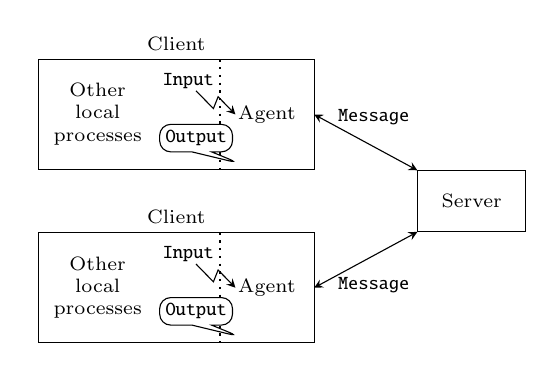
\begin{tikzpicture}[%
  >=stealth,
  msg/.style={font=\scriptsize\ttfamily},
  every node/.style={font=\scriptsize},
  client/.pic={
    \coordinate (-west) at (3.5,-0.7);
    \draw (0,0) -- (3.5,0) -- (3.5,-1.4) -- (0,-1.4) -- cycle;
    \draw[dotted,thick] (2.3,0) -- (2.3, -1.4);
    \node at (1.75,0.2) {Client};
    \node (op) at (0.75,-0.7) {
      \begin{tabular}{c}
        Other\\local\\processes        
      \end{tabular}
    };
    \node (a) at (2.9,-0.7) {
      Agent
    };
    \begin{scope}[shift={(2.5,-0.7)}, yscale=1.5]
      \draw[->] (-0.5,0.2) node[above=-1mm,shift={(-0.1,0)},msg] {Input} -- (-0.28,0.05) -- (-0.22,0.15) -- (0,0);
    \end{scope}
    \begin{scope}[shift={(2.5,-1.2)}]
      \node[inner sep=0.75mm, draw, fill=white, rectangle callout, rounded corners, callout absolute pointer={(0.05,-0.12)}, msg] (out) at (-0.5,0.2) {Output};
      % 
    \end{scope}
  }]
  \pic (c1) at (0,0) {client};
  \pic (c2) at (0,2.2) {client};
  \node[draw,inner sep=3mm] (s) at ($(c1-west)!0.5!(c2-west) + (2,0)$) {Server};
  \draw[<->] (c1-west) -- node[msg,below,shift={(0.1,-0.1)}] {Message} (s.south west);
  \draw[<->] (c2-west) -- node[msg,above,shift={(0.1,0.1)}] {Message} (s.north west);
\end{tikzpicture}


  \caption{Architecture of a lock service application. Boxes represent separate
    physical nodes, while dotted lines separate processes running on
    the same node.  Each client node runs an Agent process that
    exchanges input and output with other local processes.  The Agent
    also exchanges network messages with the Server.}

\label{fig:lock-service-architecture}
\end{figure}

To provide this API, the lock service consists of a central lock Server
node, and a lock Agent that runs on every client node, as illustrated in
\cref{fig:lock-service-architecture}.
%
That is, each client node runs a lock Agent along with other client
processes that access the API through the Agent.
%
Each lock Agent communicates over the network with the central lock server.
%
The Agent requests and releases the lock with the \LockMsg and \UnlockMsg
network messages, and the server sends a \GrantMsg network message to
notify an Agent when it has received the lock.
%
% Note that, while the network may suffer disruptions, the input/output
% messages \LockIO, \UnlockIO, and \GrantIO are sent within a node and are
% delivered reliably and in order.

% We first overview building and verifying the system in a reliable
% network where machines never crash and packets may be reordered, but
% are never dropped or duplicated.  Then we show how a verified
% system transformer can be used, \emph{without any
%   additional proof effort}, to obtain a correctness proof for this
% system in a more adversarial network where packets are dropped and
% duplicated.  More details about these network semantics are discussed
% in \cref{sec:verdi:nwsem}.

\begin{figure}[p]

\begin{lstlisting}[language=caml,basicstyle=\scriptsize\tt,morekeywords={output,send,nop}]
(* 1 - node identifiers *)
Name := Server | Agent(int)

(* 2 - API, also known as external IO *)
Inp := Lock | Unlock
Out := Grant
(* 2 - network messages *)
Msg := LockMsg | UnlockMsg | GrantMsg

(* 3 - state *)
State (n: Name) :=
  match n with
  | Server => list Name (* head = agent holding lock      *)
                        (* tail = agents waiting for lock *)
  | Agent n => bool     (* true iff this agent holds lock *)

InitState (n: Name) : State n :=
  match n with
  | Server => []
  | Agent n => false

(* 4 - handlers for external input and internal messages *)
HandleInp (n: Name) (s: State n) (inp: Inp) :=
  match n with
  | Server => nop   (* server performs no external IO *)
  | Agent n =>
    match inp with
    | Lock => (* if client requests lock, forward to Server *)
      send (Server, LockMsg)
    | Unlock => (* if client requests unlock and lock held... *)
      if s == true then (
        (* update state and tell Server lock freed *)
        s := false;;
        send (Server, UnlockMsg))

HandleMsg (n: Name) (s: State n) (src: Name) (msg: Msg) :=
  match n with
  | Server =>
    match msg with
    | LockMsg => (* if lock not held, immediately grant *)
      if s == [] then send (src, GrantMsg);;
      s := s ++ [src] (* add requestor to end of queue *)
    | UnlockMsg => (* head of queue no longer holds lock *)
      s := tail s;;
      (* grant lock to next waiting agent, if any *)
      if s != [] then send (head s, GrantMsg)
    | _ => nop (* never happens *)
  | Agent n =>
    match msg with
    | GrantMsg => (* we have the lock *)
      (* update state and notify external listeners *)
      s := true;;
      output Grant
    | _ => nop         (* never happens *)
\end{lstlisting}

\caption{A simple lock service application implemented in \Verdi, under the
  assumption of a reliable network.  \Verdi extracts these definitions into
  OCaml and links the resulting code with a runtime to send and receive
  messages over the network.}
\label{fig:lock-service-code}
\end{figure}

\subsection{Specification}

A \Verdi programmer specifies the correct behavior of their system in
terms of \textit{traces}, the sequences of external input and output
generated by nodes in the system.
%
For the lock service application, correctness requires mutual exclusion: no
two distinct nodes should ever simultaneously hold the lock.
%
This mutual exclusion property can be expressed as a predicate over traces:
%
\[ \begin{array}{l}
  \relax\property{mutex}(\tau) \coloneq \NL
  \iV \tau \;=\; \tau_1 \appop
             \tevent{n_1}{\GrantIO} \appop
             \tau_2 \appop
             \tevent{n_2}{\GrantIO} \appop
             \tau_3 \NL
  \iV \rightarrow
    \tevent{n_1}{\UnlockIO} \in \tau_2
\end{array} \]
%
To hold on trace $\tau$, the $\property{mutex}$ predicate requires that
whenever \GrantIO is output on node $n_1$ and then later \GrantIO is output
on node $n_2$, there must first be an intervening \UnlockIO input from
$n_1$ releasing the lock.

A system implementation satisfies specification $\tracespec$ in a
particular network semantics if for all traces $\tau$ the system can
produce under that semantics, $\tracespec$ holds on $\tau$.  For the
example lock service application, an implementation satisfies
\property{mutex} in a given semantics if \property{mutex} holds on all the
traces produced under that semantics.


%% {\smaller\setlength{\arraycolsep}{.5\arraycolsep}%
%% \begin{eqnarray*}
%%   \property{mutex}(\tau)\ & \mathtt{:=} & \property{mutex'}(\tau, \mathtt{None})
%%   \\
%%   \property{mutex'}([], \mathtt{None}) & \mathtt{:=} & \mathtt{true}
%%   \\
%%   \property{mutex'}([], n) & \mathtt{:=} & \mathtt{true}
%%   \\
%%   \property{mutex'}(\traceelt{n', \GrantIO} :: \tau', \mathtt{None})
%%   & \mathtt{:=} &  \property{mutex'}(\tau', n')
%%   \\
%%   \property{mutex'}(\traceelt{n', \GrantIO} :: \tau', n)
%%   & \mathtt{:=} & \mathtt{false} % \quad \text{ if } n \ne \mathtt{None}
%%   \\
%%   \property{mutex'}(\traceelt{n, \UnlockIO} :: \tau', n)
%%   & \mathtt{:=} & \property{mutex'}(\tau', \mathtt{None})
%%   \\
%%   \property{mutex'}(\traceelt{n', \UnlockIO} :: \tau', n)
%%   & \mathtt{:=}
%%   &  \property{mutex'}(\tau', n)  \quad \text{ if } n' \ne n
%%   \\
%%   \property{mutex'}(\traceelt{n', \LockIO} :: \tau', n)
%%   & \mathtt{:=} & \property{mutex'}(\tau', n)
%% \end{eqnarray*}%
%% }%

\subsection{Implementation}

Figure~\ref{fig:lock-service-code} shows the definitions a programmer
provides to implement the lock service application in \Verdi.
%
(1) \Name lists the names of nodes in the system.
%
In the lock service application, there is a single Server node and an
arbitrary number of Agents.
%
(2) \Input and \Output define the API of the lock service --- the external
input and output exchanged between an Agent and other local processes on
its node.
%
\Message defines network messages exchanged between Agents and the central
Server.
%--- this is an implementation detail of the lock service.
%
(3) \VerdiState defines the state maintained at each node.
Node state is defined as a dependent type where a node's name determines
the data maintained locally at that node.
%
In the lock service, the Server maintains a queue of Agent nodes,
initially empty, where the head of the queue is the Agent currently
holding the lock and the rest of the queue represents the Agents which
are waiting to acquire the lock.
%
Each Agent maintains a boolean, initially false, which is true exactly when
that Agent holds the lock.
%
(4) The handler functions \HandleInput and \HandleMessage define how
nodes respond to external input and to network messages.

This implementation assumes a reliable network where machines never crash
and packets may be reordered but are not dropped or duplicated.
%
These assumptions reduce the programmer's effort in both implementing the
application and proving it correct.
%
\Cref{sec:verdi:failures-locksrv} shows how \Verdi can automatically transform
the lock service application into a version that tolerates faults.

When the system runs, each node listens for events and responds by running
the appropriate handler: \HandleInput for external input and \HandleMessage
for network messages.
%
% External input
%
When an Agent receives an external input that requests to acquire or
release the lock, it forwards the request to the Server; in the \UnlockIO
case, it first checks to ensure that the lock is actually held, and it
resets its local state to \mytt{false}.
Because the network is assumed to be reliable, no acknowledgment
of the release is needed from the Server.
%
%% This feels redundant to Mike.
% Note that the Server does not act on any external input or generate
% any external output.
%
% Network messages
%
When the Server receives a \LockMsg network message, if the lock is not
held, the server immediately grants the lock, and always adds the
requesting Agent to the end of the queue of nodes.
%
When the Server receives an \UnlockMsg message, it removes a node from the
head of its queue of Agents and grants the lock to the next Agent in the
queue, if any.
%
When an Agent receives a \GrantMsg message, it produces external output
(\GrantIO) to inform other processes running on its node that the lock is
held.

The application will be deployed on some network, and \emph{network
semantics} capture assumptions about the network's behavior.
%
For this example, we assume a semantics encoding a reliable network.
%
In a reliable network, each step of execution either (1) picks an arbitrary
node and delivers an arbitrary external input, runs that node's input
handler, and updates the state, or (2) picks a message in the network, runs
the recipient's message handler, and updates the state.

Figure~\ref{fig:lock-service-diagram} shows an execution of the lock
service application with two agents.
%
Agents $A_1$ and $A_2$ both try to acquire the lock. The service first
grants the lock to $A_1$.
%
Once $A_1$ releases the lock, the service grants it to $A_2$.
%
Note that, because our network semantics does not assume messages are
delivered in the same order in which they were sent, there is a potential
race condition: an agent can attempt to re-acquire the lock before the
server has processed its previous release.
%
In that case, the server simply (and correctly) adds the sender to the
queue again.
%
Using \Verdi, the lock service is guaranteed to behave correctly even
in such corner cases.
\begin{figure}[t]
  \centering
  % \includegraphics[width=\columnwidth]{lock}
  \usetikzlibrary{backgrounds}
\usetikzlibrary{calc}
\usetikzlibrary{positioning}
\usetikzlibrary{shapes.callouts}

\def\cOneX{0}
\def\sX{2}
\def\cTwoX{4}
\begin{tikzpicture}[yscale=1.5,
  >=stealth,
  every node/.style={font=\scriptsize},
  state/.style={font=\scriptsize\bf\ttfamily},
  msg/.style={font=\scriptsize\ttfamily}
  ]
  \node (c1) at (\cOneX,0) {$A_1$};
  \node (s) at (\sX,0) {$S$};
  \node (c2) at (\cTwoX,0) {$A_2$};

  % \draw[->] (7, -1) -- node[above,rotate=90] {time} (7, -10);

  \node[state] (c1-init) at (\cOneX,-0.5) {false};
  \node[state] (s-init) at (\sX,-0.5) {[]};
  \node[state] (c2-init) at (\cTwoX,-0.5) {false};


  \def\verdiInputL#1#2{%
    {%
      \def\beginning{($#1 + (-0.5,0.2)$)}%
      \def\cOne{($#1 + (-0.28,0.05)$)}%
      \def\cTwo{($#1 + (-0.22,0.15)$)}%

      % \draw[gray] \beginning -- \cOne;%
      % \fill[gray] \cOne circle (0.2mm);%
      % \draw[gray] \cTwo -- #1;%
      % \fill[gray] \cTwo circle (0.2mm);%
      \draw[->] \beginning node[above,msg] {#2} -- \cOne -- \cTwo -- #1 ;%
    }
  }

  \def\verdiInputR#1#2{%
    {%
      \def\beginning{($#1 + (0.5,0.2)$)}%
      \def\cOne{($#1 + (0.28,0.05)$)}%
      \def\cTwo{($#1 + (0.22,0.15)$)}%

      % \draw[gray] \beginning -- \cOne;%
      % \fill[gray] \cOne circle (0.2mm);%
      % \draw[gray] \cTwo -- #1;%
      % \fill[gray] \cTwo circle (0.2mm);%
      \draw[->] \beginning node[above,msg] {#2} -- \cOne -- \cTwo -- #1 ;%
    }
  }

  \def\verdiOutputL#1#2{%
    {%
      \node[msg, draw, rectangle callout, rounded corners, callout absolute pointer={#1}, anchor=east,] at ($#1 + (0,0.3)$) {#2};
    }
  }
  \def\verdiOutputR#1#2{%
    {%
      \node[msg, draw, rectangle callout, rounded corners, callout absolute pointer={#1}, anchor=west,] at ($#1 + (0,0.3)$) {#2};
    }
  }

  \def\verdiMsgAbove#1#2#3{%
    \draw[->] #1 -- node[msg,above,yshift=1mm] {#3} #2;%
  }

  \def\verdiMsgBelow#1#2#3{%
    \draw[->] #1 -- node[msg,below,shift={(-2mm,-1mm)}] {#3} #2;%
  }

  \node[state] (c1-send-lock) at (\cOneX, -1.3) {};
  \verdiInputL{(c1-send-lock.west)}{\LockIO}

  \node[state] (s-recv-c1-lock) at (\sX, -1.8) {[$A_1$]};
  \verdiMsgAbove{(c1-send-lock)}{(s-recv-c1-lock)}{\LockMsg}
  \node[state] (c1-recv-grant) at (\cOneX, -2.3) {true};
  \verdiMsgAbove{(s-recv-c1-lock)}{(c1-recv-grant)}{\GrantMsg}
  \verdiOutputL{(c1-recv-grant.west)}{\GrantIO}

  \node[state] (c2-send-lock) at (\cTwoX, -1.5) {};
  \verdiInputR{(c2-send-lock.east)}{\LockIO}
  \node[state] (s-recv-c2-lock) at (\sX, -2.7) {[$A_1$,$A_2$]};
  \draw[->] (c2-send-lock) -- node[msg,above,yshift=4mm] {\LockMsg} (s-recv-c2-lock);%


  \node[state] (c1-send-unlock) at (\cOneX, -3) {false};
  \verdiInputL{(c1-send-unlock.west)}{\UnlockIO}

  \node[state] (s-recv-c1-unlock) at (\sX, -3.5) {[$A_2$]};
  \verdiMsgBelow{(c1-send-unlock)}{(s-recv-c1-unlock)}{\UnlockMsg}

  \node[state] (c2-recv-grant) at (\cTwoX, -4) {true};
  \verdiMsgBelow{(s-recv-c1-unlock)}{(c2-recv-grant)}{\GrantMsg}
  \verdiOutputR{($(c2-recv-grant.east) !.3! (c2-recv-grant.south east)$)}{\GrantIO}

  \draw (c1-init) -- (c1-send-lock) -- (c1-recv-grant) -- (c1-send-unlock);
  \draw (s-init) -- (s-recv-c1-lock) -- (s-recv-c2-lock) -- (s-recv-c1-unlock);
  \draw (c2-init) -- (c2-send-lock) -- (c2-recv-grant);

  \begin{scope}[shift={(-1,-4.4)},
    every node/.style={font=\scriptsize},
    outp/.style={inner sep=0.7mm,draw,rectangle callout, rounded corners, callout relative pointer={(235:3mm)}}]
    \draw[gray] (1,0) -- (5,0);
    \def\verdiInputR#1#2{%
      {%
        \begin{scope}[rotate=25]
          \def\beginning{($#1 + (0.5,0.2)$)}%
          \def\cOne{($#1 + (0.324,0.08)$)}%
          \def\cTwo{($#1 + (0.3168,0.216)$)}%
          \def\ending{($#1 + (0.10,0.072)$)}%

          % \draw[gray] \beginning -- \cOne;%
          % \fill[gray] \cOne circle (0.2mm);%
          % \draw[gray] \cTwo -- #1;%
          % \fill[gray] \cTwo circle (0.2mm);%
          \draw[->] \beginning node[inner sep=0mm,above,msg,xshift=-1mm,yshift=0.5mm] {#2} -- \cOne -- \cTwo -- \ending ;%
        \end{scope}
      }
    }

    \node (trace) at (3,-0.5) {$[\tevent{A_1}{\tikz[baseline=4.5mm]{\verdiInputR{(0,0)}{\LockIO}}},%
      \tevent{A_2}{\tikz[baseline=4.5mm]{\verdiInputR{(0,0)}{\LockIO}}},%
      \tevent{A_1}{\tikz[baseline=-0.5mm]{\draw node[inner sep=0.7mm,draw,rectangle callout, rounded corners, callout relative pointer={(235:3mm)}] {\GrantIO}}},%
      \tevent{A_1}{\tikz[baseline=4.5mm]{\verdiInputR{(0,0)}{\UnlockIO}}},%
      \tevent{A_2}{\tikz[baseline=-0.5mm]{\draw node[inner sep=0.7mm,draw,rectangle callout, rounded corners, callout relative pointer={(235:3mm)}] {\GrantIO}}}]$};
    %\node[below of=trace,node distance=2mm] (empty-filler)  {};
  \end{scope}

  % \node[state] (c2-send-unlock) at (\cTwoX, -5) {false};
  % \verdiInputR{(c2-send-unlock.east)}{\UnlockIO}
  % \node[state] (s-recv-c2-unlock) at (\sX, -5.5) {[]};
  % \verdiMsgAbove{(c2-send-unlock)}{(s-recv-c2-unlock)}{\UnlockMsg}
\end{tikzpicture}%these comments prevent extra whitespace
%

  \caption{The behavior of the lock service application, with one
    server~$S$ and two agents~$A_1$ and $A_2$.
    %
    Each agent starts with the state \mytt{false}, and the server starts
    with an empty queue.
    %
    Time flows downward.
    %
    In response to external input (drawn with lightning-bolt arrows) and
    network messages, the nodes exchange messages and update local state.
    %
    External output is shown as speech bubbles.
    %
    The trace of this execution is shown at the bottom; note that only
  externally-visible events (external input and output) appear in the trace.}

\label{fig:lock-service-diagram}
\end{figure}

\subsection{Verifying the Lock Service Application}

We briefly outline the proof of the \property{mutex} property for the lock
service application in the reliable network environment~(\ie, no machine
crashes nor packet loss/duplication).
%
The proof that \property{mutex} holds on all traces of the lock service
application consists of three high-level steps: (1) prove an invariant
about the reachable node and network states of the lock service
application, (2) relate these reachable states to the producible traces,
and (3) show that the previous two steps imply \property{mutex} holds on all
producible traces.

The first step proves that all reachable system states satisfy the
$\mutexstate$ property:
%
 \[ \begin{array}{l}
  \mutexstate(\Sigma,\ P)\ \coloneq \NL
  \iV  \forall\ n\ m,\ n \ne m \to
       \neg \property{hasLock}(\Sigma,\ n) \lor
       \neg \property{hasLock}(\Sigma,\ m) \BR
  \property{hasLock}(\Sigma,\ n)\ \coloneq \NL
  \iV  \Sigma(\mbox{Agent}(n)) = \<true>
\end{array} \]
%
The function $\Sigma$ maps node names to their state, and $P$ is the set of
in-flight packets. The property $\mutexstate$ ensures
that at most one Agent node holds the lock at a time.

A programmer can verify the $\mutexstate$ property by proving
an \textit{inductive state invariant}.
%
A property $\phi$ is an inductive invariant if both
%
(1) it holds in the initial state, $(\Sigma_0,\ \emptyset)$, where
$\Sigma_0$ maps each node to its initial state and $\emptyset$ represents
the initial, empty network, and also
%
(2) whenever it holds in some state, $(\Sigma,\ P)$, and $(\Sigma,\ P)$
can step to $(\Sigma',\ P')$, then it holds in $(\Sigma',\ P')$.

One inductive state invariant for \mutexstate is:
%
\begin{align*}
         & \left(\forall\ n,\, \property{hasLock}(\Sigma,\ n) \to \property{atHead}(\Sigma,\ n)\right)\\
  \wedge & \left(\forall\ p\in P,\ p.\<body> = \GrantMsg \to \property{grantee}(\Sigma,\ p.\<dest>)\right)\\
  \wedge & \left(\forall\ p\in P,\ p.\<body> = \UnlockMsg \to \property{grantee}(\Sigma,\ p.\<source>)\right)\\
  \wedge & ~\property{at\_most\_one}\ \{\GrantMsg,\ \UnlockMsg\}\ P
\end{align*}%
 where%
\begin{align*}
  \property{atHead}(\Sigma,\ n) \quad \coloneq & \quad \exists\ t,\ \Sigma(\mbox{Server}) = n :: t \\
  \property{grantee}(\Sigma,\ n) \quad \coloneq & \quad \property{atHead}(\Sigma,\ n) \wedge \neg \property{hasLock}(\Sigma,\ n).
\end{align*}%
%
The first conjunct above ensures that the Server and Agents agree on who
holds the lock.
%
The second and third conjuncts state that \GrantMsg is never
sent to an agent that already holds the lock, and that \UnlockMsg
is never sent from an agent that still holds the lock.
%
Finally, the last conjunct states that there is at most one in-flight
message in the set $\{\GrantMsg, \UnlockMsg\}$; this is necessary to
ensure that neither of the previous two conjuncts is violated when a
message is delivered.
%
We proved in \Coq that this invariant is inductive and that it implies
$\mutexstate$; the proof is approximately 500 lines long.


The second step of the proof relates reachable states to the traces a system
can produce:
%
\[ \begin{array}{l}
  \property{trace\_state\_agreement}(\tau,\ \Sigma)\ \coloneq \NL
  \iV  \forall\ n,\ \property{lastGrant}(\tau,\ n)
       \leftrightarrow \property{hasLock}(\Sigma,\ n) \BR
%
  \property{lastGrant}(\tau,\ n)\ \coloneq \exists\ \tau_1\ \tau_2,\NL
  \iV  \tau = \tau_1 \appop
              \tevent{n}{\GrantIO} \consop
              \tau_2 \wedge
              \forall\ m,\ \tevent{m}{\UnlockIO} \not\in \tau_2 \BR
\end{array} \]
%
This property requires that whenever a \GrantIO output appears in
the trace without a corresponding \UnlockIO input, that agent's flag is
true (and vice versa).
%
The proof of this property is by induction on the possible behavior of
the network.

The third step of the proof shows that together,
\mutexstate and \property{trace\_state\_agreement} imply
that \property{mutex} holds on all traces of the lock service
application under the reliable semantics. This result follows
from the definitions of $\property{mutex}$, $\mutexstate$,
and $\property{trace\_state\_agreement}$.

\subsection{Verified System Transformers}
\label{sec:verdi:failures-locksrv}

We have proved the \property{mutex} property for a reliable environment
where the network does not drop or duplicate packets and the server does
not crash.
%
Assuming such a reliable environment simplifies the proof by allowing the
programmer to consider fewer cases.
%
To transfer the property into an unreliable environment with network and
machine failures, a programmer uses \Verdi's verified system transformers.
%
As illustrated by Figure~\ref{fig:verdi-components} part~\numcircled{4},
after verifying a distributed system in one network semantics, a programmer
can apply a verified system transformer to produce another version of their
system which provides analogous guarantees in another network semantics.

In general, there are two types of transformers in \Verdi:
\textit{transmission transformers} that handle network faults like packet
duplication and drops and \textit{replication transformers} that handle
node crashes.
%
Below we describe an example transmission transformer for the lock
service application and briefly overview replication transformers,
deferring details to \cref{sec:verdi:casestudy-raft}.

\para{Tolerating network faults} \cref{fig:lock-service-code}'s
implementation of the lock service application will \emph{not} function
correctly in a network where messages can be duplicated.
%
If an \UnlockMsg message is duplicated but the agent reacquires the lock
before the second copy is delivered, the server will misinterpret the
duplicated \UnlockMsg message as releasing the second lock acquisition.

Realistically, most developers would not run into this issue, as
correct TCP implementations reject duplicate transmissions. However,
some distributed systems need to handle deduplication and
retransmission at a higher level, or choose not to trust the
guarantees provided by unverified TCP implementations.

As another option, a programmer could rewrite the lock service---for
instance, by including a unique identifier with
every \GrantMsg and \UnlockMsg message to ensure that they are
properly paired.
%
The developer would then need to re-prove system correctness for this
slightly different system in the semantics that models packet-duplicating
networks.
%
This would require finding a new inductive invariant and writing another
proof.

%
\Verdi allows developers to skip these steps. \Verdi provides a system
transformer that adds sequence numbers to every outgoing packet and
ignores packets with sequence numbers that have already been seen.
%
Applying this transformer to the lock service yields both a new system
\textit{and a proof} that the new system preserves the \property{mutex}
property even when packets are duplicated by the underlying network.
%
Section~\ref{sec:verdi:libraries} further details this transformer.

More generally, \Verdi decouples the verification of application-level
guarantees from the implementation and verification of fault-tolerance
mechanisms.
%
\Verdi provides a collection of verified system transformers which allow
the developer to transfer guarantees about a system in one network
semantics to analogous guarantees about a transformed version of the
system in another network semantics.
%
This allows a programmer to build and verify their system against an
idealized semantics and use a verified system transformer to obtain a
version of the system that provably tolerates more realistic faults while
guaranteeing end-to-end system correctness properties.

% The current lock service application cannot tolerate server crashes.
\para{Tolerating machine crashes}
\Verdi also provides verified system transformers to tolerate
machine crashes via replication.  Such replication transformers generally
create multiple copies of a node in order tolerate machine crashes.
%
This changes the number of nodes when transforming a system, which we
discuss further in \cref{sec:verdi:casestudy-raft}.
%
(By contrast, transmission transformers like the one described above
generally preserve the number of nodes and the relationships between them
when transforming a distributed system.)


\subsection{Running the Lock Service Application}

Now we have a formally verified lock service, written in \Coq,
that tolerates message duplication faults.
%
To obtain an executable for deployment, a \Verdi programmer invokes \Coq's
built-in extraction mechanism to generate OCaml code from the \Coq
implementation, compile it with the OCaml compiler, and link it with a
\Verdi shim.
%
The shim is written in OCaml; it implements network primitives~(e.g.,
packet send/receive) and an event loop that invokes the appropriate event
handler for incoming network packets, IO, or other events.

\subsection{Summary}

We have demonstrated how to use \Verdi to establish a strong guarantee of
the \property{mutex} property for the lock service application running in a
realistic environment.
%
Specifically, a programmer first specifies, implements, and verifies an
application assuming a reliable environment.
%
The programmer then applies system transformers to obtain a version of
their application that handles faults in a provably correct way.

\Verdi's trusted computing base includes the following components: the
specifications of verified applications, the assumption that \Verdi's
network semantics match the physical network, the \Verdi shim, \Coq's
proof checker and OCaml code extractor, and the OCaml compiler and
runtime.

\Verdi currently supports verifying safety properties, but not liveness
properties, and none of \Verdi's network semantics currently capture
Byzantine fault models.
%
We believe that \Verdi could be extended to support these features:
liveness properties could be verified by supporting infinite traces and
adding fairness hypotheses as axioms as in TLA~\cite{lamport:tla}, while
Byzantine fault models can be supported by adding more non-determinism in
the network semantics.

%%  LocalWords:  implementing-in-verdi init initState getState putState.
%%  LocalWords:  handleNet handleIO e.g. handleLocalInput enqueues boolean
%%  LocalWords:  mutex nwsem monadic Haskell-like dest VST mutex' n' pbj
%%  LocalWords:  locksrv lastGrant hasLock atHead casestudy

\section{Network Semantics}\label{sec:verdi:nwsem}

The correctness of a distributed system relies on assumptions about its
environment.
%
For example, one distributed system may assume a reliable network, while
others may be designed to tolerate packet reordering, loss, or
duplication.
%
To enable programmers to reason about the correctness of distributed
systems in the appropriate environment model, \Verdi provides a spectrum of
\emph{network semantics} that encode possible system behaviors using
small-step style derivation rules.

This section presents the spectrum of network semantics that \Verdi
provides, ranging from single-node systems that do not
rely on the network, through models of increasingly unreliable packet
delivery (reordering, drops, and duplication), and culminating with a
model that permits arbitrary node crashes under various recovery
assumptions.
%
Each of these semantics is useful for reasoning about different types of
systems.
%
For example, the properties of single-node systems can be extended
to handle node failures using protocols like
Raft, while packet duplication semantics is useful for verifying
packet delivery even in the face of reconnection, something that
raw TCP does not support.

%% To add an additional fault model to \Verdi, a programmer provides the
%% derivation rules for their network semantics, which often simply requires
%% modifying or adding inference rules to one of the semantics described
%% below.
%% %
%% As discussed later in Section~\ref{sec:verdi:libraries}, formalizing different
%% fault models as distinct network semantics played an enabling role in
%% verified system transformers, the key to modular verification in \Verdi.

\begin{figure}[t]
  \centering

  \begin{footnotesize} \begin{spacing}{1.5} \[
    \inferrule*[right=\textsc{Input}]{
      \fHinp(\sigma,\ i) = (\sigma',\ o)
    }{
      (\sigma,\ T) \fsmstep (\sigma',\ T \appop \traceelt{i,\ o})
    }
  \] \end{spacing} \end{footnotesize}

  \caption{Single-node semantics.
  %
  The derivation rule above encodes possible behaviors of a single-node
  system that does not rely on the network.
  %
  When the node is in state $\sigma$ with input/output trace $T$, it may
  receive an arbitrary input $i$, and respond by running its input handler
  $\fHinp(\sigma,\ i)$, which generates both the next state $\sigma'$ and a list of
  outputs $o$.
  %
  The \textsc{Input} rule relates the two states of the world $(\sigma,\ T) \fsmstep
  (\sigma',\ T \appop \traceelt{i,\ o})$ to reflect that the node has updated
  its state to $\sigma'$ and sent outputs $o$ in response to input $i$.
  %
  Verifying properties of such single-node systems (\ie state machines) is
useful when they are replicated over a network to provide fault tolerance.}

\label{fig:state-machine-semantics}
\end{figure}

In Verdi, network semantics are defined as step relations on a ``state of
the world''.
%
The state of the world differs among network semantics, but always includes
a trace of the system's external input and output.
%
For example, many semantics include a bag of in-flight packets
that have been sent by nodes in the system but have not yet been delivered
to their destinations.
%
Each network semantics is parameterized by system-specific data types and
handler functions.
%
Below we detail several of the network semantics \Verdi currently provides.

\paragraph{Single-node semantics} We begin with a simple semantics for
single-node systems that do not use the network, \ie state machines.
%
This semantics is useful for proving properties of single-node systems;
these can be extended, using a verified system transformer based on Raft,
to provide fault tolerance.
%
The single-node semantics, shown in \cref{fig:state-machine-semantics},
models systems of a single node that respond to input by modifying their
state and producing output.
%
The node's behavior is described by a handler \fHinp, which takes the current
local state and an input and returns the new state and a list of outputs.
%
The state of the world in this semantics is the node's state $\sigma$
paired with a trace $T$ that records the inputs sent to the system along
with the outputs the system generates.
%
The only step, \textsc{Input}, delivers an arbitrary input $i$ to the
handler $\fHinp$ and records the results in the next state.
%
The squiggly arrow between two states indicates that a system in the
state of the world on the left of the arrow may transition to the
state of the world on the right of the arrow when all of the
preconditions above the horizontal bar are satisfied. The node's state
is updated, and the trace is extended with the input $i$ and the
output $o$.

\begin{figure}[t]
  \centering

  \begin{footnotesize} \begin{spacing}{1.5} \[
    \inferrule*[right=\textsc{Input}]{
      \fHinp(n,\ \Sigma[n],\ i) = (\sigma',\ o,\ P') \\
      \Sigma' = \Sigma[n \mapsto \sigma']
    }{
      (P,\ \Sigma,\ T) \fastep (P \uplus P',\ \Sigma',\ T \appop \traceelt{i,\ o})
    }
  \]\[
    \inferrule*[right=\textsc{Deliver}]{
      \fHnet(dst,\ \Sigma[dst],\ src,\ m) = (\sigma',\ o,\ P') \\
      \Sigma' = \Sigma[dst \mapsto \sigma']
    }{
      (\{(src,\ dst,\ m)\} \uplus P,\ \Sigma,\ T) \fastep (P \uplus P',\ \Sigma',\ T \appop \traceelt{o})
    }
  \] \end{spacing} \end{footnotesize}

  \caption{Reordering semantics.
  %
  The derivation rules above encode the behavior of systems running on
  networks that may arbitrarily reorder packet delivery.
  %
  The network is modeled as a bag (\ie a multiset) $P$ of \textit{packets}, which
  contain source and destination node names as well as a message.
  The state at each node in the network is a map
  $\Sigma$ from node names to system-defined data.
  %
  The \textsc{Input} rule passes arbitrary input $i$
  to the input handler $\fHinp$ for a given node $n$ in state
  $\sigma$, which generates the next state $\sigma'$, a list of
  outputs $o$, and a multiset of new packets $P'$. The outputs are
  added to the externally-visible trace, while the packets are added
  to the network (using the multiset-union operator $\uplus$).
  %
  The \textsc{Deliver} rule works similarly, except that instead of
  running a handler in response to arbitrary input, the network handle
  $\fHnet$ is run on a packet taken from the network.
}
\label{fig:async-semantics}
\end{figure}

\paragraph{Reordering semantics}

The reordering semantics, shown in \cref{fig:async-semantics}, models a
system running on multiple nodes where packets are always delivered but
may be arbitrarily reordered.
%
This was the ``reliable'' semantics initially used for the lock
service implementation in Section~\ref{sec:verdi:overview}.
%
Each node communicates with other processes running on the same host via
input and output, just as in the single-node semantics.
%
Nodes can also exchange \textit{packets}, which are tuples of the form
(source, destination, message), over a network that may reorder
packets arbitrarily but does not drop, duplicate, or fabricate
them.
%
The behavior of nodes is described by two handler functions.
%
The input handler, \fHinp, is run whenever a node receives input from
another process on the same host.
%
\fHinp{} takes as arguments the node on which it is running, the current
local state, and the input that was delivered.
%
It returns the new local state and a list of outputs and packets to be
processed by the semantics.
%
Similarly, the network handler, \fHnet, is run whenever a packet
is delivered from the network.
%
\fHnet\ takes as arguments the receiver of the packet, the sender of the
packet, the local state, and the message that was delivered.

A state of the world in the reordering semantics consists of a bag of
in-flight packets $P$, a map from nodes to their local state $\Sigma$, and a
trace $T$.
%
The two rules in the reordering semantics, \textsc{Input} and
\textsc{Deliver}, respectively, model input from other processes on
the node's host (\ie the ``outside world'') and delivery of a packet
from the network, where the corresponding handler function executes
as described above.
%
Delivered packets are removed from the bag of in-flight packets.
%
Input and output are recorded in the trace; new packets are added to the
bag of in-flight packets.

\paragraph{Duplicating semantics}

\begin{figure}[t]

  \begin{footnotesize} \begin{spacing}{1.5} \[
    \inferrule*[right=\textsc{Duplicate}]{
      p \in P
    }{
      (P,\ \Sigma,\ T) \fdupstep (P \uplus \{p\},\ \Sigma,\ T)
    }
  \] \end{spacing} \end{footnotesize}

  \caption{Duplicating semantics.
  %
    The duplicating semantics includes all the derivation rules from
    the reordering semantics, which we elide for space. In addition,
    it includes the \textsc{Duplicate} rule, which duplicates an
    arbitrary packet in the network. This represents a simple class of
    network failure in which a network misbehaves by delivering the
    same packet multiple times.}

\label{fig:dupsem}
\end{figure}

The duplicating semantics, shown in \cref{fig:dupsem}, extends the
reordering semantics to model packet duplication in the network.
%
In addition to the \textsc{Input} and \textsc{Deliver} rules from the
reordering semantics, the duplicating semantics includes the rule
\textsc{Duplicate}, which adds an additional copy of an in-flight packet to
the network.

\paragraph{Dropping semantics}

\begin{figure}[t]
  \centering

  \begin{footnotesize} \begin{spacing}{1.5} \[
    \inferrule*[right=\textsc{Drop}]{
    }{
      (\{p\} \uplus P,\ \Sigma,\ T) \fdropstep (P,\ \Sigma,\ T)
    }
  \]\[
    \inferrule*[right=\textsc{Timeout}]{
      \fHtmt(n,\ \Sigma[n]) = (\sigma',\ o,\ P') \\
      \Sigma' =\ \Sigma[n \mapsto \sigma'] \\
    }{
      (P,\ \Sigma,\ T) \fdropstep (P \uplus P',\ \Sigma',\ T \appop \traceelt{\mathrm{tmt},\ o})
    }
  \] \end{spacing} \end{footnotesize}

  \caption{Dropping semantics.
  %
    The dropping semantics includes the two rules above in addition to all
    the derivation rules from the duplicating semantics.  The \textsc{Drop}
    rule allows a network to arbitrarily drop packets.  Systems which
    tolerate dropped packets need to retransmit some messages, so the
    dropping semantics also includes a \textsc{Timeout} rule, which fires a
    node's timeout handler $\fHtmt$.  The \Verdi shim implements this by
    setting system-defined timeouts after every event; if another event has
  not occurred on a given node before the timeout fires, the system's
$\fHtmt$ handler is executed. Note that the semantics do not explicitly
model time and allow timeouts to occur at any step.}

\label{fig:dropsem}
\end{figure}

\cref{fig:dropsem} specifies a network that drops arbitrary in-flight
packets.
%
The \textsc{Drop} rule allows any packet in the in-flight bag $P$ to be
dropped.
%
However, simply adding this rule to the semantics would make it very
difficult to write working systems, since handler functions only execute
when packets are delivered and packets may be arbitrarily dropped.
%
Real networked systems handle the possibility that packets can be dropped
by setting timeouts, which execute if a certain amount of time has elapsed
without receiving some other input or packet.
%
We model this behavior in the \textsc{Timeout} rule: a timeout can be
delivered to any node at any time, and will execute the node's $\fHtmt$
handler.

\paragraph{Node failure}

\begin{figure}[t]
  \centering

  \begin{footnotesize} \begin{spacing}{1.5} \[
    \inferrule*[right=\textsc{Crash}]{
      n \not\in F
    }{
      (P,\ \Sigma,\ F,\ T) \ffailstep (P,\ \Sigma,\ \{n\} \cup F,\ T)
    }
  \]\[
    \inferrule*[right=\textsc{Reboot}]{
      n \in F \\
      \fHrbt(n,\ \Sigma[n]) = \sigma' \\
      \Sigma' =\ \Sigma[n \mapsto \sigma'] \\
    }{
      (P,\ \Sigma,\ F,\ T) \ffailstep (P,\ \Sigma',\ F - \{n\},\ T)
    }
  \] \end{spacing} \end{footnotesize}

  \caption{Failure semantics.
  %
    The node failure semantics represents a network in which nodes can both
    stop and start, and adds a set of failed nodes $F$ to the state of the
    world.
    %
    The node failure semantics includes all the derivation rules from the
    dropping semantics in addition to the rules above.
    %
    The rules from the drop semantics are modified to only run when node
    $n$ is not in the set of failed nodes $F$.
    %
    The \textsc{Crash} rule simply adds a node to the set of failed nodes
    $F$.
    %
    Crashed nodes may re-enter the network via the \textsc{Reboot} rule, at
  which point their state is restored according to the $\fHrbt$ function.}

\label{fig:failure-semantics}
\end{figure}

There are many possible models for node failure.
%
Some systems assume that nodes will always return after a failure, in which
case node failure is equivalent to a very long delay.
%
Others assume that nodes will never return to the system once they have
failed.
%
\Verdi's semantics for node failure, illustrated in
\cref{fig:failure-semantics} assumes that nodes can return to the system
and that all, some, or none of their state will be preserved (\ie read back
in from non-volatile storage).
%
The state of the world in the node failure semantics includes a set $F$
containing the nodes which have failed.
%
The rules from the drop semantics are included in the failure semantics,
but each with an added precondition to ensure that only live nodes (\ie
nodes that are not in $F$) can receive external input, network packets, or
timeouts.
%
A node can fail (be added to $F$) at any time, and failed nodes can return
at any time.
%
When a failed node returns, the $\fHrbt$ (reboot) function is run on its
pre-failure state to determine what state survives the failure.

\paragraph{Low-level details}

\Verdi's network semantics currently elide low-level network details.
%
For example, input, output, and packets are modeled as abstract datatypes
rather than bits exchanged over wires, and system details such as
connection state are not modeled.
%
This level of abstraction simplifies \Verdi's semantics and eases both
implementation and proof.
%
Lower-level semantics could be developed and connected to the semantics
presented here via system transformers, as described in the next section.
%
This would further reduce \Verdi's trusted computing base and increase our
confidence in the end-to-end guarantees \Verdi provides.

\section{Verified System Transformers}
\label{sec:verdi:libraries}

\begin{figure}
  \centering
  {
\begin{tikzpicture}[thick,
  every node/.style={align=center,font={}}]
  \matrix[row sep=1.5cm,column sep=1.5cm] {
  % First row:
  \node (SA) {$S_A$}; & \node (PA) {$\Phi(S_A)$}; \\
  % Second row:
  \node (SB) {$S_B$}; & \node (PB) {$\mathrm{lift}(\Phi)(S_B)$}; \\
  };
  \draw[-{Stealth[]},double,double distance=2pt] (SA) -- node[left=2mm] {transformer} (SB);
  \draw[-{Stealth[]},double,double distance=2pt] (PA) -- node[right=2mm] {transformer\\correctness} (PB);
\end{tikzpicture}
}

  \caption{A verified system transformer takes a system ($S_A$) written
    against some network semantics and returns a new system ($S_B$) in
    another semantics. Its correctness property states that for any
    property $\Phi$ of the original system, a lifted version of that
    property holds on the transformed system.}
  \label{fig:vst}
\end{figure}
\todo{Incorporate \cref{fig:vst}.}

\Verdi's spectrum of network semantics enable the programmer to reason
about their system running in the fault model corresponding to their
environment. However, directly verifying a system in a realistic fault
model requires establishing both application-level guarantees and the
correctness of fault-tolerance mechanisms simultaneously.  \Verdi
provides verified system transformers to separate these concerns and
enable a modular approach to building and verifying distributed
systems. The programmer can assume an idealized network while
verifying application-level guarantees and then apply a transformer to
obtain a system that tolerates more faults while providing analogous guarantees.

For common fault models, the distributed systems community has
developed standard techniques to handle failures. For example, as
discussed in \cref{sec:verdi:overview}, by adding a unique sequence
number to every message and ignoring previously received messages,
systems can handle packet duplication. \Verdi supports such
standard fault-tolerance mechanisms through verified system transformers,
which \emph{transform} systems from one semantics to another while
guaranteeing that analogous system properties are preserved. For
example, in the transformer that handles deduplication, any property
that holds on the underlying system is true of the transformed
system when sequence numbers are stripped away.

System transformers are implemented as wrappers around the system's state,
messages, and handlers. Messages and state are generally transformed to
include additional fields.  Handlers in the transformed system call into
underlying handlers and implement additional functionality.  The underlying
handlers are called with underlying state and underlying messages,
capturing the intuition that the underlying handlers are unable to
distinguish whether they are running in their original network semantics or
the new semantics targeted by the system transformer.

System transformers in \Verdi are generally either
\textit{transmission transformers}, which tolerate network faults by
adding functionality to every node in a system, or \textit{replication
  transformers}, which tolerate node failures by making several copies
of the underlying nodes. The sequence numbering transformer discussed
below is an example of a transmission
transformer. \cref{sec:verdi:casestudy-pbj,sec:verdi:casestudy-raft} discuss
replication transformers.

\subsection{Sequence Numbering Transformer}

\begin{figure}
\begin{lstlisting}[language=caml,basicstyle=\scriptsize\tt,morekeywords={output,send,nop}]
(* S describes a system in the reordering semantics *)
SeqNum (S) :=
  Name := S.Name

  Inp := S.Inp
  Out := S.Out
  Msg := { seqnum: int; underlying_msg: S.Msg }

  State (n: Name) := { seen: list (Name * int);
                       next_seqnum: int;
                       underlying_state: S.State n }

  InitState (n: Name) := { seen := [];
                           next_seqnum := 0;
                           underlying_state := S.InitState n }

  HandleInp (n: Name) (s: State n) (inp: Inp) :=
    wrap_result (S.HandleInp (underlying_state s) inp)

  HandleMsg (n: Name) (s: State n) (src: Name) (msg: Msg) :=
    if not (contains s.seen (src, msg.seqnum)) then
      s.seen := (src, msg.seqnum) :: s.seen;;
      (* wrap_result adds sequence numbers to messages while
         incrementing next_seqnum *)
      wrap_result (S.HandleMsg n (underlying_state s)
                               src (underlying_msg msg))

\end{lstlisting}
\caption{Pseudocode for the sequence numbering transformer.}
\label{fig:seqnum}
\end{figure}

Sequence numbering is a technique for ensuring that messages are
delivered at most once. Senders tag each outgoing message with a
sequence number that is unique among all messages from that
sender. Message recipients keep track of all
\traceelt{\mytt{number},\ \mytt{sender}} pairs they have seen.  If a message arrives with a
\traceelt{\mytt{number},\ \mytt{sender}} pair that the destination has
seen before, the message is discarded.

\cref{fig:seqnum} shows the \Verdi implementation of the sequence
numbering transformer, \mytt{SeqNum}. It takes a distributed system
$S$ as input and produces a new distributed system that implements
sequence numbering by wrapping the message, state, and handler
definitions in $S$. \mytt{SeqNum} leaves the \Name, \Input, and
\Output types unchanged. It adds an integer field to each message
which is used as a sequence number to uniquely identify
messages. \mytt{SeqNum} also adds a list of (\Name, \mytt{int}) pairs
to the state to track the sequence numbers received from other nodes
in the system, as well as an additional counter to track the local
node's current maximum sequence number. The initial state in the
wrapped system is constructed by building the initial state for the
underlying system and then setting all sequence numbers to zero. To
handle messages, the wrapped handler checks the input message to
determine if it has previously been processed: if so, the message is
simply dropped; otherwise, the message is passed to the message
handler of $S$. Messages sent by the underlying handler are paired
with fresh sequence numbers and the sequence number counter is
incremented appropriately using the helper function
\mytt{wrap\_result}. The input handler passes input through to the
input handler from $S$ and wraps the results.

\subsection{Correctness of Sequence Numbering}
\label{sec:verdi:correctness:sequence-numbering}

Given a proof that property $\Phi$ holds on every trace of an
underlying system, the correctness of a system transformer should
enable a programmer to easily establish an analogous property $\Phi'$ of traces
in the transformed system.

Each verified system transformer $T$ provides a function $\transfer$
which translates properties of traces in the underlying semantics $\fstepOne$
to the target semantics $\fstepTwo$:
%
\begin{align*}
  \forall\ \Phi\ S,\  & \mbox{\mytt{holds}}(\Phi,\ S,\ \fstepOne) \to \\
                      & \mbox{\mytt{holds}}(\transfer(\Phi),\ T(S),\ \fstepTwo)
\end{align*}
%
where $\mytt{holds}(\Phi,\ S,\ \leadsto)$ asserts that a
property $\Phi$ is true of all traces of a system $S$ under the
semantics defined by $\leadsto$. Crucially, the \mytt{transfer}
function defines how properties of the underlying system are
translated to analogous properties of the transformed system.

For the sequence numbering transformer, $\fstepOne$ is $\fastep$ (the
step relation for the reordering semantics) and $\fstepTwo$ is
$\fdupstep$ (the step relation for the duplicating semantics). The
\mytt{transfer} function is the identity function: properties of
externally visible traces are precisely preserved by the
transformation. Intuitively, the external output
depends only on the wrapped state of the system, and the wrapped state
is preserved by the transformer.

We prove that the wrapped state is preserved by \emph{backward
simulation}: for any step the transformed system $T(S)$ can take, the
underlying system $S$ can take an equivalent step. We specify this using
helper functions $\unwrap$ and $\dedupnet$. Given the global state of
the transformed system, $\unwrap$ returns the underlying state at each
node.  Given the global state of the transformed system and the bag of
in-flight messages, $\dedupnet$ returns a bag of packets which
includes only those messages which will actually be delivered to the
underlying handlers---non-duplicate packets which have not yet been
delivered. The simulation is specified as follows, where
$\fdupstepstar$ and $\fastepstar$ are the reflexive transitive
closures of the duplicating semantics and the reordering semantics, respectively:
\begin{align*}
  &(\Sigma_0,\ \emptyset,\ \emptyset) \fdupstepstar (\Sigma,\ P,\ T) \to \\
  &(\unwrap(\Sigma_0),\ \emptyset,\ \emptyset) \fastepstar (\unwrap(\Sigma),\ \dedupnet(\Sigma, P),\ T)
\end{align*}
The proof is by induction on the step relation. For
\textsc{Duplicate} steps, $\fastepstar$ holds reflexively, since
$\dedupnet$ returns the same network when a packet is
duplicated and the state and trace are unchanged.
For \textsc{Deliver} steps, the proof shows that
either the delivered packet is ignored by the destination node, in
which case $\fastepstar$ holds reflexively, or that the underlying
handler is run normally, in which case the underlying system can take
the analogous \textsc{Deliver} step. For both the \textsc{Deliver} and
\textsc{Input} steps, the proof shows that wrapping the sent packets
results in a deduplicated network that is reachable in the underlying
system. These proofs require several facts about the internal state of
the sequence numbering transformer, such as the fact that all nodes
correctly maintain their \mytt{next\_seqnum} field. These internal
state properties are proved by induction on the execution.

\subsection{Ghost Variables and System Transformers}

Many program verification frameworks support
\textit{ghost variables}: state which is never read during
program execution, but which is necessary for verification (\eg to
provide sufficiently strong induction hypotheses). In \Verdi, ghost
variables are implemented via a system transformer. Like the sequence
numbering transformer, the ghost variable transformer adds information
to the system's state while ensuring that the wrapped state is
preserved. The system's original handlers are called in order to
update the wrapped state and send messages; the new handlers only
update the ghost state. The indistinguishability result shows that the
ghost transformer does not affect the externally-visible trace or the
wrapped state. In this way, ghost state can be added to \Verdi systems
for free, without requiring any additional proof effort to show
that properties verified in the ghost system hold for the underlying
system as well.

\section{Case Study: Key-Value Store}\label{sec:verdi:casestudy-kvstore}

\newcommand{\getk}{\<get>\xspace}
\newcommand{\putk}{\<put>\xspace}
\newcommand{\delk}{\<delete>\xspace}

As a case study, we implemented a simple key-value store as a single-node
system in \Verdi. The key-value store accepts \getk, \putk, and \delk
operations as input.  When the system receives input $\getk(k)$, it outputs
the value associated with key $k$; when the system receives input $\putk(k,\ v)$, it
updates its state to associate key $k$ with value $v$; and when the system
receives input $\delk(k)$, it removes any associations for the key $k$ from its
state.  Internally, the mapping from keys to values is represented using an
association list.
%\footnote{A more realistic implementation would use a hash table or an
%efficient tree structure.}

The key-value store's correctness is specified in terms of traces. First,
operations on a single key are specified using an interpreter over trace
input/output events, which
runs each operation and returns the final result.  For instance,
\begin{align*}
  \<interpret>&\;[ \,\putk \; \mbox{\small{\text{``foo''}}}
  , \; \putk \; \mbox{\small{\text{``bar''}}}  , \; \getk  ] = \mbox{\small\text{``bar''}}
\end{align*}

Trace correctness is then defined using the interpreter: for every
\traceelt{\<input>,\ \<output>} pair in the trace,
\<output> is equal to the value returned by running the
interpreter on all operations on that key up to that point.
This trace-based specification allows the programmer to change the
backing data structure and implementation of each operation
without changing the system's specification. Moreover, additional
operations can be added to the specification via small modifications to the
interpretation function.

We prove the key-value store's correctness by relating its trace to
its current state: for all keys, the value in the association list for
that key is equal to interpreting all the operations on that key in
the trace. The proof is by induction on the execution, and is
approximately 280 lines long.

In the next section, we will see how a state-machine replication
system can be implemented and verified using \Verdi. Combining the
key-value store with the replication transformer provides an
end-to-end guarantee for a replicated key-value store without
requiring the programmer to simultaneously reason about both
application correctness and fault tolerance.

\section{Case Study: Primary-Backup Transformer}\label{sec:verdi:casestudy-pbj}

\begin{figure}[t]
  \centering
  \begin{lstlisting}[language=caml,basicstyle=\scriptsize\tt,morekeywords={output,send,nop}]
PB (S) :=
  Name := Primary | Backup

  Msg := Replicate S.Inp | Ack
  Inp := S.Inp
  Out := { request: S.Inp; response: S.Out }
  State (n: Name) = { queue: list S.Inp;
                      underlying_state: S.State }

  InitState (n: Name) = { queue := [];
                          underlying_state := S.InitState n }

  HandleInp (n: Name) (s: State n) (inp: Inp) :=
    if n == Primary then
      append_to_queue inp;;
      if length s.queue == 1 then
        (* if not already replicating a request *)
        send (Backup, Replicate (head s.queue))

  HandleMsg (n: Name) (s: State n) (src: Name) (msg: Msg) :=
    match n, msg with
      | Primary, Ack =>
        out := apply_entry (head s.queue);;
        output { request := head s.queue; response := out };;
        pop s.queue;;
        if s.queue != [] then
          send (Backup, Replicate (head s.queue))
      | Backup, Replicate i =>
        apply_entry i;;
        send (Primary, Ack)

  \end{lstlisting}

  \caption{Pseudocode for the primary-backup transformer. The primary node
    accepts commands from external input and replicates them to the backup
    node.  During execution, the primary node keeps a queue of operations
    it has received but not yet replicated to the backup node. The backup
    node applies operations to its local state and notifies the primary node.
    Once the primary node receives a notification, it responds to the client.}

\label{fig:pbj-code}
\end{figure}

In this section, we introduce the primary-backup replication transformer,
which takes a single-node system and returns a replicated version of the
system in the reordering semantics. A primary node synchronously replicates
requests to a backup node: when a request arrives, the primary ensures that
the backup has processed it before applying it locally and replying to the
client. Whenever a client gets a response, the corresponding request has
been processed by both the primary and the backup. Pseudocode for the
primary-backup transformer is shown in~\cref{fig:pbj-code}.

The primary-backup transformer's correctness is partially specified in
terms of traces the primary may produce: any sequence of inputs and
corresponding outputs produced by the primary node is a sequence that could
have occurred in the original single-node system, and thus any property
$\Phi$ of traces of the underlying single-node system also holds on all
traces at the primary node in the transformed system. This result
guarantees indistinguishability for the primary-backup transformer.

The primary-backup transformer specification also relates the backup node's
state to the primary node's state. Because the primary replicates entries
synchronously, and one at a time, the backup can fall arbitrarily behind
the input stream at the primary. However, the primary does not send a
response to the client until the backup has replicated the corresponding
request. Thus, the state at the backup is closely tied to that at the
primary. In particular, we were able to show that either the primary and
the backup have the same state or the backup's state is one step ahead of
the primary.  This property provides some intuitive guarantees about
potential failure of the primary: namely, that manual intervention could
restore service with the guarantee that any lost request must not have been
acknowledged. It makes sense that manual intervention is necessary in the
case of failure: the composed system is verified against the reordering
semantics, where the developer assumes that machine crashes require manual
intervention.

%\subsection{A replicated key-value store}\label{ssec:verdi:kv+pbj}

Once implemented and verified, the primary-backup transformer can be used
to construct replicated applications. Applying it to the case study from
\cref{sec:verdi:casestudy-kvstore} results in a replicated key-value store. The
resulting system is easy to reason about because of the transformer's
indistinguishability result. For example, we were able to show (in
about 10 lines) that submitting a \putk request results in a response that
correctly reflects the \putk.

\section{Case Study: Raft Replication Transformer}
\label{sec:verdi:casestudy-raft}

Fault-tolerant, consistent state machine replication
is a classic problem in distributed systems.
This problem has been
solved with \textit{distributed consensus} algorithms, which guarantee
that all nodes in a system will agree on which commands the replicated
state machine has executed and in what order, and that each node has a
consistent copy of the state machine.

In \Verdi, we can implement consistent state machine replication as a
system transformer. The consistent replication transformer lifts a
system designed for the state machine semantics into a system that
tolerates machine crashes in the failure semantics. We implemented the
replication transformer using the Raft consensus
algorithm~\cite{ongaro:raft}. Our implementation of Raft in \Verdi is
described in~\cref{ssec:verdi:raft-impl}.

A \Verdi system transformer lifts a safety property of an input
system into a new semantics. The consensus transformer provides an
indistinguishability result for \textit{linearizability}, which states
that any possible trace of the replicated system is equivalent to some
valid trace of the underlying system under particular constraints
about when operations can be re-ordered. We have proved that Raft's
\textit{state machine safety} property implies linearizability.
We also verified the (much more difficult) state machine safety property
for Raft~\cite{Woos-al:CPP16}.
We discuss these results further in~\cref{ssec:verdi:raft-proof}.

\subsection{Raft Background}\label{ssec:verdi:raft-background}

Raft is a \textit{state machine replication protocol}.
The state machine is a deterministic program that specifies
the desired behavior of the cluster as a whole.
The state machine processes a sequence of \emph{commands},
which are given by the clients of the cluster.
External clients interact with
the system as if it were a single node running
a single copy of the state machine.

Each node in a Raft cluster simulates a copy of the state machine,
and the goal of the protocol is to maintain consistency across the copies.
Replication allows the system to continue
serving clients whenever a majority of machines are available.
%because the remaining machines can continue.
However, maintaining consistency among replicas
is difficult in the presence of asynchrony,
network failures (packet drops, duplications, and reordering)
and node failures (crashes and reboots).
In particular, the combination of asynchrony and failure means that
the nodes in the system are never guaranteed
to be in global agreement~\cite{flp}.

Since Raft requires that the
state machine it replicates is deterministic,
the replicas will be consistent
as long as the same client commands
are executed on each replica's copy in the same order.
Raft's main internal correctness invariant,
called state machine safety,
captures this property.
\begin{proposition}[State Machine Safety]\label{prop:sms}
  Each replicated copy of the state machine executes the same commands in the same order.
\end{proposition}

The list of commands to execute on the state machine
is kept in the \emph{log},
and the position of a command in the log is called its \emph{index}.
Each node has its own copy of the log,
and state machine safety reduces to maintaining agreement between
all copies of the log.

\begin{figure}
  \centering
  {
\def\rhs{6}
\def\nOne{1} % This is actually node 3!
\def\nTwo{2}
\def\nThree{3} % This is actually node 1!
\def\start{0}
\def\bx{0.5}
\def\cx{1}
\def\dx{1.3}
\def\ex{1.8}
\def\fx{2.3}
\def\gx{2.4}
\def\hx{2.9}
\def\ix{3.4}
\def\jx{3.65}
\def\kx{3.9}
\def\lx{4.4}
\def\mx{4.9}
\def\nx{5.2}
\def\axisy{0.7}
\begin{tikzpicture}[>=stealth, thick,
  every node/.style={font={\scriptsize}},
  msg label/.style={}]
  \draw[->] (-0.2,\axisy) -- ($(\rhs,0.7) + (0.2,0)$) node[below] {time};
  \draw[dashed] (0,\nOne)   node[xshift=-1mm, left] {node 3} -- ($(\jx,\nOne) + (-.1, 0)$);
  \draw[dashed] (0,\nTwo)   node[xshift=-1mm, left] {node 2} -- (\rhs,\nTwo) node[right] {$\ldots$};
  \draw[dashed] (0,\nThree) node[xshift=-1mm, left] {node 1} -- (\rhs,\nThree);

  \draw[->] (\start,1) -- node[msg label, left, near end, xshift=.5mm] {RV} (\bx, 3);
  \draw[->] (\start,1) -- (\bx, 2);
  \draw[->] ($(\bx, 3) + (0.05, 0)$) -- node[msg label, right, near start, xshift=-.5mm] {V} (\cx, 1);
  \coordinate (drop1) at ($(\bx, 2)!.6!(\cx, 1)$);
  \draw[-{Rays[red]}] ($(\bx, 2) + (0.05, 0)$) -- (drop1);

  \draw[very thick, orange, densely dotted] ($(\start, 1) + (-0.1, -0.1)$) rectangle ($(\cx, 3) + (0.1, 0.1)$);

  \draw[->] (\dx,1) -- node[msg label, left, near end, xshift=.5mm] {AE} (\ex, 3);
  \draw[->] (\dx,1) -- (\ex, 2);

  \draw[->] ($(\ex, 3) + (0.05, 0)$) -- node[msg label, right, near start, xshift=-.5mm] {Ack} (\fx, 1);
  \draw[->] ($(\ex, 2) + (0.05, 0)$) -- (\fx, 1);

  \draw[->] (\gx,1) -- (\hx, 3);
  \draw[->] (\gx,1) -- (\hx, 2);

  \coordinate (drop2) at ($ ($(\hx, 3) + (0.05, 0)$) ! 0.4 ! (\ix, 1)$);

  \draw[-{Rays[red]}] ($(\hx, 3) + (0.05, 0)$) to (drop2);
  \draw[->] ($(\hx, 2) + (0.05, 0)$) -- (\ix, 1);

  \draw[very thick, blue, densely dotted] ($(\dx, 1) + (-0.1, -0.1)$) rectangle ($(\ix, 3) + (0.1, 0.1)$);

  \draw[red] ($(\jx, \nOne)$) circle[radius=.6mm];

  \draw[->] (\kx, 3) -- (\lx, 2);
  \draw[->] (\kx, 3) -- (\lx, 1);
  \draw[->] ($(\lx, 2) + (0.05, 0)$) -- (\mx, 3);

  \draw[very thick, orange, densely dotted] ($(\kx, 1) + (-0.1, -0.1)$) rectangle ($(\mx, 3) + (0.1, 0.1)$);

  \draw[very thick, blue, densely dotted] ($(\nx, 1) + (-0.1, -0.1)$) -- ++ (0, 2.2) -- ($(\rhs, 3) + (0.1, 0.1)$)
                                          ($(\nx, 1) + (-0.1, -0.1)$) -- ($(\rhs, 1) + (0.1, -0.1)$);



  %\draw (\start, \axisy) ++ (0,-0.1) node[below] {\mkevent{A}\theeventnum}  -- ++ (0,0.2);
  %\draw (\bx, \axisy) ++ (0,-0.1) node[below] {\mkevent{B}\theeventnum}  -- ++ (0,0.2);

  % \draw let \p1 = (drop1) in
  %   (\x1, \axisy) ++ (0,-0.1) node[below,yshift=0.06mm] {\mkevent{C}\theeventnum}  -- ++ (0,0.2);

  %\draw (\cx, \axisy) ++ (0,-0.1) node[below] {\mkevent{D}\theeventnum}  -- ++ (0,0.2);
  \draw (\dx, \axisy) ++ (0,-0.1) node[below] {\mkevent{event:request}\theeventnum}  -- ++ (0,0.2);
  \draw (\ex, \axisy) ++ (0,-0.1) node[below] {\mkevent{event:request-received}\theeventnum}  -- ++ (0,0.2);
  \draw (\fx, \axisy) ++ (0,-0.1) node[below] {\mkevent{event:commit}\theeventnum}  -- ++ (0,0.2);

  \draw let \p1 = (drop2) in
    (\x1, \axisy) ++ (0,-0.1) node[below] {\mkevent{event:drop}\theeventnum}  -- ++ (0,0.2);

  %\draw (\ix, \axisy) ++ (0,-0.1) node[below] {\mkevent{H}\theeventnum}  -- ++ (0,0.2);
  \draw (\jx, \axisy) ++ (0,-0.1) node[below] {\mkevent{event:crash}\theeventnum}  -- ++ (0,0.2);
  \draw (\kx, \axisy) ++ (0,-0.1) node[below] {\mkevent{event:timeout}\theeventnum}  -- ++ (0,0.2);
  %\draw (\mx, \axisy) ++ (0,-0.1) node[below] {\mkevent{K}\theeventnum}  -- ++ (0,0.2);


  \draw[decorate,decoration={brace}] (0,3.4) ++ (-0.1, 0) -- node[above,yshift=1mm] {term 1} ($(\ix, 3.4) + (0.1, 0)$);
  \draw[decorate,decoration={brace}] (\kx,3.4) ++ (-0.1, 0) -- node[above,yshift=1mm] {term 2} ($(\rhs, 3.4) + (0.3, 0)$);
  \fill[white] ($(\rhs, 3.4) + (0.1, -0.1)$) rectangle ($(\rhs, 3.4) + (0.4, 0.1)$);
  \draw (\bx,3.275) node[anchor=center] {election};
  \draw (\fx,3.275) node[anchor=center] {replication};
  \draw (\lx,3.275) node[anchor=center] {election};
\end{tikzpicture}
}

  \caption[Terms in Raft]{Two terms of the Raft protocol, each consisting of a leader election phase (orange)
    followed by a log replication phase (blue).
    Node 3 is the leader of the first term, and node 1 is the leader of the
    second term.
  Messages are RequestVote (RV),
Vote (V), AppendEntries (AE), or Acknowledgment (Ack).
\tikz[thick]{ \draw[-{Rays[red]}] (0,0) -- (0.1,0); }
represents a dropped message and
\tikz[thick]{ \draw[red] ($(0, 0)$) circle[radius=.6mm]; }
represents a crashed node.
}
  \label{fig:raft-overview}
\end{figure}

\cref{fig:raft-overview} shows an example execution of the Raft
protocol.\footnote{\url{https://raft.github.io/} has a visualization of Raft in operation.}
Time is logically divided into \emph{terms},
and each term consists of a leader election phase
followed by a log replication phase.
During leader election, the cluster chooses a \emph{leader},
who coordinates the cluster and handles all communication with clients
during the following log replication phase.
Nodes are either leaders, \emph{candidates}, or \emph{followers}.
Candidates are in the process of trying to become leader.
Followers passively obey the leader of the current term and respond to
\texttt{RequestVote} messages from candidates.

\paragraph*{Leader Election}
If the leader node crashes or is isolated by a network
partition (\eg, node 3 at \cref{event:crash} in \cref{fig:raft-overview}),
the Raft system elects a new leader.
When a node times out waiting to hear from a leader
(as node 1 does at \cref{event:timeout} in \cref{fig:raft-overview}),
it becomes a candidate.\footnote{Timeouts are randomized and configured so that candidates rarely compete for leadership. See Ongaro's thesis for more detail on the leader election process~\cite{ongaro:phd}.}
A candidate tries to get itself elected as the new leader
by sending messages requesting votes from all other nodes.
Once a candidate receives votes from a majority of nodes in the system,
it becomes the leader.
If no candidate successfully wins the election,
a new election will take place following a timeout.
Requiring a majority ensures that there is only one leader elected per term.
\begin{proposition}[Election Safety]
  There is at most one leader per term.
\end{proposition}

\paragraph*{Log Replication}
During normal operation,
  the cluster is in the log replication phase.
In log replication,
  when a client sends an input to
  the leader\footnote{Raft implementations have various mechanisms
    for clients to locate the leader. In our implementation, clients
    can send their operations to every node in the cluster until the
    leader is found.}
  (\eg, at \cref{event:request} in \cref{fig:raft-overview}),
  the leader first appends a new \emph{log entry}
  containing that command to its local log.
Then the leader sends an \emph{AppendEntries} message
  containing the entry to the other nodes in the Raft system.
Each other node appends the entries to its log
  (\eg, at \cref{event:request-received} in \cref{fig:raft-overview}),
  and responds to the leader with an acknowledgment.
To ensure that follower logs stay consistent
  with the log at the leader,
  AppendEntries messages include the index and term
  of the \textit{previous} entry in the leader's log;
  the follower checks that
  it too has an entry at that index and term
  before appending the new entries to its log.
This consistency check guarantees the following property:
\begin{proposition}[Log Matching]
  If two logs contain entries at a particular index and term,
  then the logs are identical up to and including that index.
\end{proposition}


Once the leader learns that a majority of nodes (including itself)
have received the new entry
(\eg, at \cref{event:commit} in \cref{fig:raft-overview}),
the leader marks the entry as \emph{committed}.\footnote{Committing
  old entries (those from leaders who failed before completely
  replicating them) is more complex; see the Raft
  paper~\cite{ongaro:raft} for details.}
Note that the leader need not receive acknowledgments
from all nodes before proceeding
(\eg, an acknowledgment is dropped at \cref{event:drop} in \cref{fig:raft-overview},
but nodes 2 and 3 constitute a majority).
The leader then executes the command contained in the committed entry on the state machine and
responds to the client with the output of the command.
The followers are also informed that they can safely execute
the command on their state machines.

Once an entry is committed, it becomes \emph{durable},
in the sense that its effect will never be forgotten by the cluster.
To ensure that leader elections do not violate this property,
a new leader must have heard of
all committed entries created by the previous leader.
Therefore, Raft specifies that a node only votes for candidates whose
log is at least as advanced as the voter's.
Because a newly elected leader was voted in by a majority,
it has a log that is at least as advanced
as a majority of the cluster.
Since any committed entry is present on a majority,
every committed entry is present on at least one node that voted for the candidate.
The successful candidate's log thus contains every committed entry.
\begin{proposition}[Leader Completeness]\label{prop:leader-completeness}
  A successfully elected candidate's log contains every committed entry.
\end{proposition}

\paragraph*{Client-facing correctness}
Clients expect to interact with Raft nodes
as if the nodes were collectively a single state machine.
More formally, clients see a
\textit{linearizable} view of the replicated state~\cite{herlihy:linearizability},
\ie, if any node responds to a client command $c$,
all subsequently requested commands will execute on a state machine
that reflects the execution of $c$.
\cref{ssec:verdi:raft-proof} gives a precise definition of linearizability.
\begin{proposition}
  Raft implements a linearizable state machine.
\end{proposition}

Raft also provides a liveness guarantee:
if there are sufficiently few failures,
then the system will eventually process and respond to
all client commands.
To date, we have only verified Raft's safety properties,
leaving liveness for future work.

\subsection{Raft Implementation}\label{ssec:verdi:raft-impl}

\begin{figure}[ht!]
  \centering
  \small
\begin{lstlisting}[language=caml,basicstyle=\scriptsize\tt,morekeywords={output,send,nop}]
input := ClientRequest (c : cmd) (uid : nat)...

output := ClientResponse (uid : nat) (r : result) ...
        | NotLeader

handleInput (i : input) :=
  match i with
  | ClientRequest ...
  end;
  leaderHeartbeat();
  executeEntries()

(* internal Raft messages *)
msg := RequestVote ...
     | Vote ...
     | AppendEntries ...
     | Acknowledgment ...

handleMessage (m : msg) :=
  match m with
  | AppendEntries ...
  | Acknowledgment ...
  | RequestVote ...
  | Vote ...
  end;
  leaderHeartbeat();
  executeEntries()

handleTimeout :=
   ...; leaderHeartbeat(); executeEntries()

leaderHeartbeat :=
  (* send AppendEntries to followers *)
  (* mark entries as committed *)
  ...

executeEntries :=
  (* execute entries on the local state machine *)
  (* respond to clients if necessary *)

logEntry := { c     : cmd;
              index : nat;
              term  : nat; ... }

nodeType := Leader | Candidate | Follower

data := { log : list logEntry;
          commitIndex : nat;
          term : nat;
          type : nodeType;
          sm : stateMachine; ... }

init : data := { log := [];
                 commitIndex := 0;
                 term := 0;
                 type := Follower;
                 sm := initialStateMachine; ... }
\end{lstlisting}
  \caption{Signatures of key parts of our Raft implementation.}
\label{fig:raft-pseudocode}
\end{figure}

We implemented Raft as a verified system transformer
from a single node semantics with no faults
to a multi-node semantics with network and machine faults.
To use the transformer,
a programmer first implements an algorithm as a (non-distributed) state machine
in which a single process responds to input from the outside world.
Then, Raft transforms this into a system where the original state machine
is consistently replicated across a number of nodes.
As a result, the programmer can prove properties about the replicated system
by reasoning only about the underlying state machine.
The Raft transformer produces a system that is proven correct in
an environment in which
all messages can be arbitrarily reordered, duplicated, delayed, or dropped,
and in which nodes can crash and reboot.
These faults correspond to the real world failure scenarios
that Raft is designed to tolerate.

\cref{fig:raft-pseudocode} shows signatures for key parts of
Raft as implemented in Verdi.\footnote{For
    more detail, see \texttt{raft/Raft.v} at
    \url{https://github.com/uwplse/verdi/tree/cpp2015}.}
There are two classes of messages:
\textit{external} messages (inputs from clients) and
\textit{internal} messages exchanged between nodes in the system.

Raft has three kinds of external messages.
Nodes running Raft receive \texttt{ClientRequest} messages from external clients;
each such message contains a command of type \texttt{cmd},
which is a parameter of the system. These are delivered in the
\texttt{step\_input} step in \cref{fig:failure-semantics}.\todo{is this the right figure to cite}
Nodes respond with \texttt{NotLeader}
to indicate that the client should find the current leader
or \texttt{ClientResponse}, containing the result of the command,
once the system has successfully processed a client command.
To ensure that network failures do not cause
a single client command to be executed multiple times,
each \texttt{ClientRequest} includes a unique identifier,
shown as \texttt{uid} in \cref{fig:raft-pseudocode}.
Raft guarantees that a request with a given identifier
will only be executed once.
Clients can thus repeatedly retry a request;
when a client receives a \texttt{ClientResponse}
with the same \texttt{uid},
it knows the command has executed exactly once on the state machine.

Raft has four kinds of internal messages:
\texttt{AppendEntries} and \texttt{Acknowledgment},
used in log replication,
and \texttt{RequestVote} and \texttt{Vote},
used in leader election.
These messages correspond directly to the behavior described
in \cref{ssec:verdi:raft-background}.

\begin{sloppypar}
Our Raft implementation consists of event handlers
for external messages, internal messages, and timeouts.
Each of these handlers begins with some event-specific code
and then calls two bookkeeping functions,
\texttt{leaderHeartbeat} and \texttt{executeEntries}.
\texttt{leaderHeartbeat} performs leader-specific tasks,
such as sending \texttt{AppendEntries} messages to followers
and marking entries as committed.
\texttt{executeEntries} performs tasks
that should be done by every server,
such as executing committed entries on the state machine.
\end{sloppypar}


The local state of each Raft node is given in \cref{fig:raft-pseudocode}
by the type \texttt{data}
and includes the log,
the index of the most recently committed entry,
the node's current term,
the node's type (\texttt{Leader}, \texttt{Candidate}, or \texttt{Follower}),
and its copy of the state machine.
The log is a list of entries,
each of which contains
a command to be executed on the state machine,
its index (position in the log),
and the term in which the entry was initially received by the cluster.

The initial state of each node is given
  by the value \texttt{init}.
The log is initially empty,
  no entries are committed,
  the current term is 0,
  every node is a follower
  (nodes will time out and start an election in term 1 to determine the first leader),
  and the state machine is in its initial state,
  having not yet processed any commands.

Our verified implementation of Raft in Coq
  consists 530 lines of code
  and 50,000 lines of proof,
  excluding code from
  the core Verdi framework. It does not support extensions to Raft
  which are useful in practice, such as dynamic reconfiguration and
  log compaction. It also includes more data on \texttt{Acknowledgment}
  messages than is necessary. These limitations are not fundamental,
  but addressing them would increase the proof burden.


\hrule\todo{merge with old PLDI text below}

\begin{table}
  \centering
  \caption{Messages, inputs, and outputs used in \Verdi's implementation of Raft.}\vspace{6pt}
  \begin{tabular}{lll}\toprule
    & \textbf{Name} & \textbf{Purpose} \\\midrule
    \multirow{4}{*}{\textbf{Messages}} & \mytt{AppendEntries} &
                                         \multirow{2}{*}{Log Replication} \\
                      & \mytt{AppendEntriesReply} & \\
                      & \mytt{RequestVote} & \multirow{2}{*}{Leader Election} \\
                      & \mytt{RequestVoteReply} & \\\midrule
    \textbf{Inputs}   & \mytt{ClientRequest} & Client inputs \\\midrule
    \multirow{2}{*}{\textbf{Outputs}}  & \mytt{ClientResponse} &
                                                                   Successful execution \\
                      & \mytt{NotLeader} & Resubmit \\\bottomrule
  \end{tabular}
\label{fig:raft-messages}
\end{table}

Raft is structured as a set of remote procedure calls (RPCs). In
\Verdi, we implement each RPC as a pair of messages. Raft's
\mytt{message} type is shown in \cref{fig:raft-messages}. Raft
divides time into \textit{terms} of arbitrary length, and guarantees
that there can be at most one leader per term. If a node $n$ suspects
that the leader has failed, that node advances its term and attempts
to become the leader by sending \mytt{RequestVote} messages to every
other node in the system. If a quorum of nodes votes for $n$, then $n$
becomes the leader for its term. Since nodes can only vote for one
leader in a given term, there is guaranteed to be at most one leader per
term.

Once a leader has been elected, it can begin replicating log
entries. A log entry stores a command (\ie an input) for the
underlying state machine, as well as the term in which it was created
and a monotonically increasing \mytt{index}. Entries are created by
the leader in response to \mytt{ClientRequest} inputs. When the
leader creates an entry $e$, it sends \mytt{AppendEntries} messages
to every other node in order to replicate $e$ in other nodes'
logs. Once $e$ is in a quorum of logs, its command can safely be
executed against the underlying state machine. More details about Raft
can be found in the original Raft paper~\cite{ongaro:raft} and
Ongaro's thesis~\shortcite{ongaro:phd}.

The \Verdi implementation of Raft includes the basic Raft algorithm,
but does not include extensions of Raft which are described in the
paper and useful in practice. In particular, it does not include log
compaction, which allows a server to garbage-collect old log entries
to save space, or membership changes, which allow nodes to be added
and removed from a Raft cluster. We leave these features for future
work.

\subsection{Raft Proof}\label{ssec:verdi:raft-proof}
The behavior of a Verdi system is described by \emph{traces},
   which record the interaction between the system and its clients.
Internal messages sent between nodes of the system
  are \emph{not} included in the trace,
  as they are not observable by clients of the cluster.
For example, if Raft is used to replicate a simple key-value store,
  a valid trace of the resulting system might be:
\begin{verbatim}
     [ClientRequest (Put "x" "hello") 1;
      ClientResponse 1 "";
      ClientRequest (Get "x") 2;
      ClientResponse 2 "hello"].
\end{verbatim}
In this execution, a client first sends a \texttt{ClientRequest}
  containing a command to set the key \verb|"x"| to the value \verb|"hello"|;
  this request is assigned the unique identifier 1.
The system then sends a response containing the empty string as its result,
  which serves as an acknowledgment that the \texttt{Put} has taken place.
The client then sends a request to read the value of the key \verb|"x"|;
  the request is assigned the unique identifier 2.
Finally, the system responds with the value \verb|"hello"|.

The correctness of a system \textit{transformer} such as Raft
  is a \textit{relation} that must hold between
  the traces generated by the transformed system
  and those generated by the original system.
In \cref{fig:vst}, this relation is called \textit{lift}.

\todo{clarify traces: types are tricky.}
The relational specification of the Raft transformer
  is that the traces it generates \textit{linearize}
  (see below)
  to traces generated by the single-node state machine.
Intuitively, linearizability means that once
  the Raft cluster sends a \texttt{ClientResponse} for a command $c$,
  the execution of all subsequently issued commands will reflect the execution of $c$.
More precisely, a trace of a replicated system linearizes to a trace
of the underlying system if its operations can be reordered to match
the underlying trace without moving an incoming command before a
previously acknowledged command.
For example, in Raft, the system can reorder concurrently issued client requests,
  but if a request is received after a previous request is acknowledged,
  then the system must respect that ordering.
% In other words, linearizable systems give clients
%   a view of a consistent sequence of commands.

We formalize the linearizes-to relation as follows.\footnote{The relevant Coq development is \texttt{raft/Linearizability.v} at \url{https://github.com/uwplse/verdi/tree/cpp2015}.}
\begin{definition}[Linearizes-to]\label{def:lin-eq}
Let $\tau$ be a trace of inputs and outputs,
where each input-output pair is given a unique key.
Then $\tau$ \textit{linearizes to}
a sequence of state machine commands $\sigma$ if
the events of $\tau$ can be reordered into a trace $\tau'$ such that
\begin{enumerate}
\item $\tau'$ is sequential,
  \ie, it consists of alternating inputs and outputs with matching keys;
\item $\tau'$ agrees with $\sigma$,
  \ie, they consist of the same sequence of commands,
       and each output in $\tau'$ equals the result given
       by the corresponding command in $\sigma$; and
\item\label{item:lin-eq-ord} if an output $o$ appears in $\tau$
  before an input $i$,
  then $o$ also appears before $i$ in $\tau'$.
\end{enumerate}
\end{definition}
Note that this definition requires $\tau$ and $\sigma$
  to contain the same set of commands.
Thus, we can define linearizability:
\begin{definition}[Linearizability]
  A trace $\tau$ is linearizable if
  there exists a sequence $\sigma$ of state machine commands
  such that $\tau$ linearizes to $\sigma$.
\end{definition}

This definition captures the notion of linearizability,
  but establishing it directly for Raft would be difficult
  because it would require strengthening it
  to be an inductive invariant of the system.
Instead, we proved Raft linearizable by relating
  the system's trace to the local state of each node
  and the set of packets in the network.

First, we related the trace of the system
  to each node's local copy of the state machine
  via state machine safety (\cref{prop:sms} from \cref{ssec:verdi:raft-background}).\todo{check that this references is correct}
%  which states that
%  each state machine executes the same commands in the same order.
Proving linearizability from state machine safety required
  proving each of the conditions in \cref{def:lin-eq}
  by reducing each to an internal property of Raft.
\todo{I just commented out the following sentence. how is the flow now?}
%We discuss our mechanism for proving such relations
%  in more detail in \cref{sec:trace-relations}.
\begin{theorem}
  State machine safety implies linearizability.\footnote{This argument is formalized in \texttt{raft/RaftLinearizableProofs.v}, along with the lemmas imported by that file.}
\end{theorem}
\begin{proof}
  Given an execution trace $\tau$ of Raft,
    we must find $\sigma$ such that $\tau$ linearizes to $\sigma$.
  There is an obvious choice for $\sigma$:
    it is just the sequence of commands executed by the nodes
    on their local state machines.
  State machine safety guarantees that the nodes agree on this sequence,
    so our choice is well defined.

  It remains to show that $\tau$ linearizes to $\sigma$.
  In other words, we must find $\tau'$ such that
    the conditions of \cref{def:lin-eq} are satisfied.
  Let $\tau'$ be the sequential input--output trace corresponding to $\sigma$,
    \ie, for each command of $\sigma$,
    $\tau'$ contains an input immediately followed by the corresponding output
    for that command.
  Then $\tau'$ is sequential and agrees with $\sigma$ by construction,
    and it remains to show that $\tau'$ is
    a permutation of $\tau$ that respects the ordering condition
    (item~\ref{item:lin-eq-ord}) of \cref{def:lin-eq}.
  Each of these is established as a separate invariant by induction on the execution.
\end{proof}

This result was formalized and proved as part of our work
  on verified system transformers~\cite{verdi}. \todo{reword verdi cite}
The remainder (and vast majority) of our Raft verification effort
  establishes state machine safety.
Since each node executes commands on its
  state machine as entries become committed in the node's log,
  state machine safety requires that nodes never disagree
  about committed entries.
The proof of State Machine Safety requires
  the use of \textit{ghost variables}.
Ghost variables are components of system state that are
tracked for the purposes of verification but not
needed at run time. This state is therefore not tracked in the extracted
implementation. For more information, see the Verdi paper~\cite{verdi}. \todo{reword verdi cite}

\begin{theorem}[State Machine Safety]
  State machine safety holds for every reachable state of the system.\footnote{The top-level proof is in \texttt{raft-proofs/StateMachineSafetyProof.v}. The ghost variables required are specified in \texttt{raft/RaftRefinement\allowbreak Interface.v} and \texttt{raft/RaftMsgRefinementInterface.v}.}
\end{theorem}
\begin{proof}[Proof Sketch]
  First strengthen the induction hypothesis
  to quantify over ghost state
  and appropriately constrain each node's history.
  Next proceed by induction on the step relation,
  and in each case show that the strengthened hypothesis is preserved.
\end{proof}

\begin{figure}
  \centering
  \small
\begin{lstlisting}[language=caml,basicstyle=\scriptsize\tt,morekeywords={output,send,nop}]
ghostData := {
  (* list of term, candidate this node voted for,
     log at time of vote *)
  votes : list (nat * name * list logEntry);

  (* term -> list of nodes who voted for
     this node in that term *)
  cronies : nat -> list name;

  (* term, log when this node became leader *)
  leaderLogs : list (nat * list logEntry);

  (* list of term, entry:
     all entries ever present in log at this node*)
  allEntries : list (nat * logEntry)
}

ghostHandleMessage (m : msg) :=
  match m with
  | AppendEntries ... =>
    (* If entries added to log, add to allEntries
       and tag with current term *)
  | RequestVote ...
    (* If voting, add the current term,
       the candidate's name,
       and the current log to votes *)
  | Vote ...
    (* Add sender to cronies at current term *)
    (* If node becomes leader, add current term
       and log to leaderLogs *)
  end
\end{lstlisting}
  \caption{Ghost variables used in the verification of Raft}
  \label{fig:raft-ghost-variables}
\end{figure}

The proof of State Machine Safety requires several ghost variables on
local data, as well as one on messages. \cref{fig:raft-ghost-variables} shows
pseudocode for the local data ghost state, including the ways in which
it is updated in response to incoming messages. Intuitively, each
ghost variable stores part of the system's \textit{history}, which is
not tracked in the actual implementation but which is necessary for
proofs. For example, a node in the system does not actually need to
keep a record of every vote that it has every cast; it is sufficient
to track only the vote for its current term. However, in order to
prove that only one leader is elected per term, the proof uses the
\texttt{votes} ghost variable.  We use the ghost state to establish
the Election Safety and Leader Completeness properties, from which we
then prove State Machine Safety. As an example, we show how Election
Safety follows using these ghost variables.\footnote{The proof of Leader
Completeness is available in \texttt{raft-proofs/\allowbreak LeaderCompletenessProof.v}.}

\begin{theorem}[Election Safety]
  Election safety is true in every reachable state of the
  system.\footnote{See \texttt{raft-proofs/OneLeaderPerTermProof.v}.}
\end{theorem}
\begin{proof}[Proof Sketch]
  If a node is a leader, then it has a majority of nodes in its
  \texttt{cronies} for that term. A node $h$ does not appear in
  \texttt{cronies} at a node $h'$ unless $h'$ is in \texttt{votes} at
  $h$ for the same term. A node only votes for one leader for each
  term. If there are two leaders for one term, at least one node $h$
  must be in \texttt{cronies} at both leaders since they each have a
  majority. That node must have voted for both of them at that term,
  so they must be the same node. Therefore, Election Safety holds.
\end{proof}

\hrule\todo{merge with PLDI15 text below}

\begin{figure}[t]
  \centering
  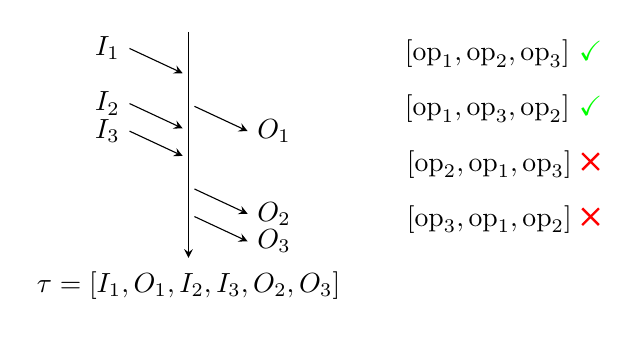
\begin{tikzpicture}[%
  >=stealth, yscale=0.7,
  hole/.style={inner sep=0.5mm}]
  \coordinate (start) at (0,-0.2) {};
  \coordinate (i1) at (0,-1) {};
  \coordinate (o1) at (0,-1.5) {};
  \coordinate (i2) at (0,-2) {};
  \coordinate (i3) at (0,-2.5) {};
  \coordinate (o2) at (0,-3) {};
  \coordinate (o3) at (0,-3.5) {};
  \coordinate (end) at (0,-4.3) {};

  \def\inp#1#2{%
    \draw[->] ($(-0.75, 0.5) + #1$) node[left] {#2} -- ($(-0.075, 0.05) + #1$);
  }

  \def\outp#1#2{%
    \draw[->] ($(0.075, -0.05) + #1$) -- ($(0.75, -0.5) + #1$) node [right] {#2};
  }

  \inp{(i1)}{$I_1$}
  \inp{(i2)}{$I_2$}
  \inp{(i3)}{$I_3$}

  \outp{(o1)}{$O_1$}
  \outp{(o2)}{$O_2$}
  \outp{(o3)}{$O_3$}

  \newcommand{\Cross}{$\mathbin{\tikz [x=1.4ex,y=1.4ex,line width=.2ex, red] \draw (0,0) -- (1,1) (0,1) -- (1,0);}$}%

  \newcommand{\Checkmark}{$\color{green}\checkmark$}

  \draw[->] (start) -- (i1) -- (o1) -- (i2) -- (i3) -- (o2) -- (o3) -- (end);

  \begin{scope}[shift={(4,-0.6)}]
    \def\op{\ensuremath{\mathrm{op}}}
    \node (t1) at (0,0) {$[\op_1, \op_2, \op_3]$\ \Checkmark};
    \node (t2) at (0,-1) {$[\op_1, \op_3, \op_2]$\ \Checkmark};
    \node (t3) at (0,-2) {$[\op_2, \op_1, \op_3]$\ \Cross};
    \node (t4) at (0,-3) {$[\op_3, \op_1, \op_2]$\ \Cross};
  \end{scope}

  \node (tau) at (0, -4.8) {$\tau = [I_1, O_1, I_2, I_3, O_2, O_3]$};
\end{tikzpicture}


  \caption{An example trace, with permitted and forbidden operation
    orderings. Since $O_1$ happens before $I_2$ and $I_3$,
    $\mathrm{op}_1$ must happen before $\mathrm{op}_2$ and
    $\mathrm{op}_3$. The operations $\mathrm{op}_2$ and
    $\mathrm{op}_3$, however, can happen in either order.}

\label{fig:linearizability-diagram}
\end{figure}


As discussed above, the indistinguishability result for Raft is
linearizability. Linearizability~\cite{herlihy:linearizability}
guarantees that clients see a consistent view of the state machine:
clients see a consistent order in which operations were executed, and
any request issued after a particular response is guaranteed to be
ordered after that response.

We verified linearizability of the \Verdi Raft implementation as a
consequence of Raft's state machine safety property, which
states that every node applies the same state machine command at a
given index. We believe that this is the first formal proof
(machine-checked or otherwise) of Raft's linearizability. A proof that
state machine safety holds for our implementation
has also been completed~\cite{verdi-repo}.
The state machine safety proof was considerably more challenging
than initially estimated and led to reusable insights on the
broader challenge of ``proof engineering''~\cite{Woos-al:CPP16}.
A pencil and paper proof of state machine
safety for a TLA model of Raft was given in Ongaro's
thesis~\shortcite{ongaro:phd}.

We formalized a general theory of linearizable systems in Coq as
follows. A trace $\tau$ of requests $I_1,\dots,I_n$ and responses
$O_1,\dots,O_m$ (where there is a total ordering on requests and
responses) is linearizable with respect to an underlying state machine
if there exists a trace of \textit{operations} (\ie request and
response pairs) $\tau'$ such that: (1) $\tau'$ is a valid, sequential
execution of the underlying state machine (meaning that each response
is the one produced by running the state machine on the trace); (2)
every response in $\tau$ has a corresponding operation in $\tau'$; and
(3) if a response to an operation $\mathrm{op}_1$ occurs before a
request for an operation $\mathrm{op}_2$ in $\tau$, then
$\mathrm{op}_1$ occurs before $\mathrm{op}_2$ in $\tau'$. Some
examples of permitted and forbidden $\tau'$ for a particular $\tau$
are shown in \cref{fig:linearizability-diagram}. Note that the
primary-backup transformer described in \cref{sec:verdi:casestudy-pbj}
trivially provides linearizability: its traces are traces of the
underlying system and it does no reordering.

Raft's I/O trace consists of \mytt{ClientRequest}s and
\mytt{ClientResponse}s. The key to the proof is that Raft's internal
log contains a linearized ordering of operations. The desired
underlying trace, then, is just the list of operations in the order of
the log. The rest of the proof involves showing that this order of
operations satisfies the conditions above. To prove condition (1), we
show that the state machine state is correctly managed by Raft and
that entries are applied in the order they appear in the
log. Condition (2) follows from the fact that Raft never issues a
\mytt{ClientResponse} before the corresponding log entry is applied to
the state machine. Finally, condition (3) holds because Raft only
appends entries to the log: if a \mytt{ClientResponse} has already
been issued, then that entry is already in the log, so any subsequent
\mytt{ClientRequest} will be ordered after it in the log.

\section{Evaluation}
\label{sec:verdi:eval}

This section aims to answer the following questions:
\begin{itemize}%[itemsep=2pt,topsep=2pt]
\item How much effort was involved in building the case studies discussed above?
\item To what extent do system transformers mitigate proof burden when
  building modular verified distributed applications?
\item Do \Verdi applications correctly handle the faults they are designed to tolerate?
\item Can a verified \Verdi application achieve reasonable performance
  relative to analogous unverified applications?
\end{itemize}

\subsection{Verification Effort}
\begin{table}[t]
  \centering
  \caption{Verification effort:  size of the specification, implementation,
    and proof, in lines of code (including blank lines and comments).}\vspace{6pt}
\label{tab:effort}
  \begin{tabular}{lrrrr}
\toprule
\textbf{System}        & \textbf{Spec.} & \textbf{Impl.} & \textbf{Proof}\\\midrule
Sequence numbering     &  20            & 89             & 576       \\
Key-value store        &  41            & 138            & 337       \\
Primary-backup         &  20            & 134            & 1155      \\
KV+PB                  &  5             & N/A            & 19        \\
Raft (Linearizability) &  170           & 520            & 4144      \\
Raft (SMS)             &  47            & N/A            & 50719     \\
Verdi                  &  148           & 220            & 2364      \\
\bottomrule
  \end{tabular}
\end{table}

\cref{tab:effort} shows the size of the
specification, implementation, and proof of each case study.
The \Verdi row shows
the number of lines in the shim,
the network semantics from \cref{sec:verdi:nwsem},
and proofs of reusable, common lemmas in \Verdi. The KV+PB row shows
the \textit{additional} lines of code required to state and prove a
simple property of the key-value store with the primary-backup
transformer applied. This line shows that verified system transformers
mitigate proof burden by preserving properties of their input systems.

\subsection{Verification Experience}

While verifying the case studies, we discovered several serious errors in
our system implementations.  The most subtle of these errors came from our
implementation of Raft: servers could delete committed entries when a
complex sequence of failures occurred. Such a sequence is unlikely to arise
in regular testing, but proving Raft in \Verdi forced us to reason about
all possible executions. The Raft linearizability property we proved
prevents such subtle errors from going unnoticed.

\subsection{Verification and Performance}

We applied the consensus transformer described in
\cref{sec:verdi:casestudy-raft} to the key-value store described in
\cref{sec:verdi:casestudy-kvstore}; we call the composed system
\vard.\footnote{Pronounced \emph{var-DEE}.} We performed a simple
evaluation of its performance.
%
We ran our benchmarks on a three-node cluster, where each node had
eight 2.0~GHz Xeon cores, 8~GB main memory, and 7200~RPM, 500~GB hard
drives.  All the nodes were connected to a gigabit switch and had ping
times of approximately 0.1~ms.
%
First, we ran the composed system and killed the leader node;
the system came back as expected.
%
Next, we measured the throughput and latency of the composed
system and compared it to etcd~\cite{etcd}, a production
fault-tolerant key-value store written in the Go language which also
uses Raft internally.
%
We used a
separate node to send 100 random requests using 8~threads; each
request was either a put or a get on a key uniformly selected from a
set of 50 keys.

\begin{table}[t]
  \centering
  \caption{A performance comparison of etcd and our \vard.}\vspace{6pt}

  \label{tab:bench}
  \begin{tabular}{r@{~~}c@{~~}c@{~~}c@{~~}}
\toprule
    %\multirow{2}{*}{\textbf{System}}
    & \multirow{2}{*}{
      \begin{tabular}{c}
        \textbf{Throughput} \\(req./s)
      \end{tabular}
    }  &
         \multicolumn{2}{c}{\textbf{Latency}}\\
    &  & \mytt{get} (ms)\;\; & \mytt{put} (ms) \\\midrule
    \mytt{etcd} & 38.9 & 205 & 198 \\
    \mytt{vard} & 34.3  & 232 & 232 \\
\bottomrule
  \end{tabular}
\end{table}

%We found that for both etcd and our key-value store, the hard
%drive was the limiting factor on throughput and latency.

As shown in \cref{tab:bench}, \vard achieves comparable performance to
etcd. We believe that etcd has slightly better throughput and latency
because of better data structures and because requests are
batched. \vard is not feature complete with respect to etcd, which
uses different internal data structures and a more complex network
protocol. Nonetheless, we believe this benchmark shows that a verified
\Verdi application can achieve roughly equivalent performance compared
to existing, unverified alternatives.
%shows that, for systems such as fault-tolerant key-value stores where
%I/O dominates performance, \Verdi applications can be competitive with
%existing alternatives.

%had slightly better throughput but lower latency. This makes sense:
%etcd is multithreaded and can parallelize client communication, but
%sends more total data over the wire and uses HTTP for both internal
%and external communication (the shim uses UDP internally and TCP
%externally).

\section{Related Work}\label{sec:verdi:related}

This section relates \Verdi to previous approaches for building
reliable distributed systems.

\begin{sloppypar}
\para{Proof assistants and distributed systems}
EventML \cite{rahli:eventml} provides expressive primitives and
combinators for implementing distributed systems.  EventML programs
can be automatically abstracted into formulae in the Logic of Events,
which can then be used to verify the system in
NuPRL~\cite{constable:nuprl}.  The ShadowDB project implements a
total-order broadcast service using
EventML~\cite{schiper:shadowdb}. The implementation is then translated
into NuPRL and verified to correctly broadcast messages while
preserving causality.  A replicated database is implemented on top of
this verified broadcast service.  Unlike \vard (described in
\cref{sec:verdi:eval}), the database itself is unverified.
\end{sloppypar}

\citeauthor{tcp-hol}~\shortcite{tcp-hol} used HOL4 to develop a detailed model and
specification for TCP and the POSIX sockets API, show that their model
implements their specification, and validate their model against
existing TCP implementations.  Rather than verifying the network stack
itself, in \Verdi we chose to focus on verifying high-level
application correctness properties against network semantics that are
assumed to correctly represent the behavior of the network
stack. These two lines of work are therefore complementary.

\citeauthor{ridge-2009}~\shortcite{ridge-2009} verified a
significant component of a distributed message queue, written in
OCaml. His technique was to develop an operational semantics for OCaml
which included some basic networking primitives, encode those
semantics in the HOL4 theorem prover, and prove that the message queue
works correctly under those semantics. Unlike in \Verdi, the proofs
for the system under failure conditions were done only on paper.

\Verdi's system transformers enable decomposing both systems and proofs.
This allows developers to establish end-to-end correctness guarantees of
the implementation of their distributed systems, from the low-level network
semantics to a high-level replicated key-value store, while retaining
flexibility and modularity. The system transformer abstraction could
integrated into these other approaches; for example, ShadowDB's consensus
layer could be implemented as a system transformer along the lines of
\Verdi's Raft implementation.

\para{Ensemble}
Ensemble~\cite{hayden:ensemble} layers simple \textit{micro protocols}
to produce sophisticated distributed systems. Like Ensemble micro
protocols, \Verdi's system transformers implement common patterns in
distributed systems as modular, reusable components.  Unlike Ensemble,
\Verdi's systems transformers come with correctness theorems that
translate guarantees made against one network semantics to analogous
guarantees against another semantics.  Unlike \Verdi, Ensemble enables
systems built by stacking many layers of abstraction to achieve
efficiency equivalent to hand-written implementations via
cross-protocol optimizations. These micro protocols are manually
translated to IO automata and verified in
NuPRL~\cite{liu:ensemble-nuprl,ensemble-verification}. In contrast,
\Verdi provides a unified framework that connects the implementation
and the formalization, eliminating the formality gap.

\para{Verified SDN} Formal verification has previously been applied to
software-defined networking, which allows routing configurations to be
flexibly specified using a simple domain specific language (see, \eg
Verified NetCore~\cite{guha:verified-openflow}).  As in \Verdi,
verifying SDN controllers involves giving a semantics for OpenFlow,
switch hardware, and network communication. The style of formalization
and proof in Verified NetCore and Verdi are quite similar and address orthogonal
problems. Verified NetCore is concerned with correct routing protocol
configuration, while Verdi is concerned with the correctness of
distributed algorithms that run on top of the network.

\para{Specification Reasoning}
There are many models for formalizing and specifying the correctness
of distributed systems~\cite{ioautomata,petrinets,pi-calculus}. One of the most
widely used models is TLA, which enables catching protocol bugs during
the design phase~\cite{lamport:thinking}.  For example, Amazon
developers reported their experience of using TLA to catch
specification bugs~\cite{Newcombe-al:CACM14}.  Another approach of finding
specification bugs is to use a model checker.  For example,
\citeauthor{zave:chord-alloy} applied Alloy~\cite{jackson:alloy} to
analyzing the protocol of the Chord distributed hash
table~\cite{zave:chord-alloy}. \citeauthor{Lynch:1996:DA:525656}~\shortcite{Lynch:1996:DA:525656}
describes algorithm transformations which are similar to \Verdi's
verified system transformers.

On the other hand, \Verdi focuses on ensuring that implementations
are correct.  While this includes the correctness of the underlying
algorithm, it goes further by also showing that the actual running
system satisfies the intended properties.

\para{Model checking and testing} There is a rich literature in
debugging distributed systems.  Run-time checkers such as
Friday~\cite{geels:friday} and D$^3$S~\cite{liu:d3s} allow developers
to specify invariants of a running system and detect possible
violations on the fly or offline.  Model checkers such as
Mace~\cite{killian:mace, killian:macemc}, MoDist~\cite{yang:modist},
and CrystalBall~\cite{yabandeh:crystalball} explore the space of
executions to detect bugs in distributed systems.  These tools are
useful for catching bugs and easy to use for developers, as they only
need to write invariants.  On the other hand, \Verdi's proofs provide
correctness guarantees.

For example, Mace provides a full suite of tools for building and model
checking distributed systems.  Mace's checker has been applied to discover
several bugs, including \emph{liveness} violations, in previously deployed
systems. Mace provides mechanisms to explicitly break abstraction
boundaries so that lower layers in a system can notify higher layers of
failures.  \Verdi does not provide liveness guarantees nor mechanisms to
break abstraction boundaries, but enables stronger guarantees via full
formal verification.

\para{Verification} Several major systems implementations have been
verified fully formally in proof assistants.  The CompCert C
compiler~\cite{leroy:compcert} was verified in
Coq and repeatedly shown to be more reliable than traditionally
developed compilers~\cite{yang:csmith,vu:emi}. Our system transformers
are directly inspired by the translation proofs in CompCert, but
adapted to handle network semantics where faults may occur.

The Reflex framework~\cite{ricketts:reflex} provides a domain-specific
language for reasoning about the behavior of reactive systems.  By
carefully restricting the DSL, the authors were able to achieve high
levels of proof automation.  Bedrock~\cite{chlipala:bedrock} and
Ynot~\cite{nanevski:ynot} are verification frameworks based on
separation logic and are useful for verifying imperative programs in
Coq, but also consider only the behavior of a single node and do not
model faults.

% These frameworks consider only the behavior of a single
% node and do not model faults.

\section{Conclusion}\label{sec:verdi:conclusion}

This chapter presented \Verdi, a framework for building formally
verified distributed systems.  \Verdi's key conceptual contribution is
the use of verified system transformers to separate concerns of
application correctness and fault tolerance, which simplifies the task
of implementing and verifying distributed systems end-to-end. This
modularity is enabled by \Verdi's encoding of distinct fault models as
separate network semantics.  We demonstrated how to apply \Verdi to
writing and verifying several practical applications, including the
Raft state replication library and the \vard fault-tolerant key-value
store, with the help of verified system transformers.  These
applications provide strong correctness guarantees and acceptable
performance while imposing reasonable verification burden. We believe
that \Verdi provides a promising first step toward our overarching
goal of easing the burden for programmers to implement correct,
high-performance, fault-tolerant distributed systems.

\chapter{Disel}

\newcounter{tagz}

% colors
\definecolor{shadecolor}{gray}{1.00}
\definecolor{darkgray}{gray}{0.30}
\definecolor{violet}{rgb}{0.56, 0.0, 1.0}
\definecolor{forestgreen}{rgb}{0.13, 0.55, 0.13}

% Col language definition
\lstdefinelanguage{Coq} {
mathescape=true,						
texcl=false,
morekeywords=[1]{
  Add,
  All,
  Arguments,
  Axiom,
  Bind,
  Canonical,
  Check,
  Close,
  CoFixpoint,
  CoInductive,
  Coercion,
  Contextual,
  Corollary,
  Defined,
  Definition,
  Delimit,
  End,
  Example,
  Export,
  Fact,
  Fixpoint,
  Goal,
  Graph,
  Hint,
  Hypotheses,
  Hypothesis,
  Implicit,
  Implicits,
  Import,
  Inductive,
  Lemma,
  Let,
  Local,
  Locate,
  Ltac,
  Maximal
  Module,
  Morphism,
  Next,
  Notation,
  Obligation,
  Open,
  Parameter,
  Parameters,
  Prenex,
  Print,
  Printing,
  Program,
  Projections,
  Proof,
  Proposition,
  Qed,
  Record,
  Relation,
  Remark,
  Require,
  Reserved,
  Resolve,
  Rewrite,
  Save,
  Scope,
  Search,
  Section,
  Show,
  Strict,
  Structure,
  Tactic,
  Theorem,
  Unset,
  Variable,
  Variables,
  View,
  inside,
  outside
},
morekeywords=[2]{
  as,
  cofix,
  else,
  end,
  exists,
  exists2,
  fix,
  for,
  forall,
  fun,
  if,
  in,
  is,
  let,
  match,
  nosimpl,
  of,
  return,
  struct,
  then,
  vfun,
  with
},
morekeywords=[3]{Type, Prop, Set, True, False},
morekeywords=[4]{
  after,
  apply,
  assert,
  auto,
  bool_congr,
  case,
  change,
  clear,
  compute,
  congr,
  cut,
  cutrewrite,
  destruct,
  elim,
  field,
  fold,
  generalize,
  have,
  heval, 
  hnf,
  induction,
  injection,
  intro,
  intros,
  intuition,
  inversion,
  left,
  loss,
  move,
  nat_congr,
  nat_norm,
  pattern,
  pose,
  refine,
  rename,
  replace,
  revert,
  rewrite,
  right,
  ring,
  set,
  simpl,
  split,
  suff,
  suffices,
  symmetry,
  transitivity,
  trivial,
  unfold,
  unlock,
  using,
  without,
  wlog,
  autorewrite
},        
morekeywords=[5]{
  assumption,
  by,
  contradiction,
  done,
  exact,
  lia,
  gappa,
  omega,
  reflexivity,
  romega,
  solve,
  tauto,
  discriminate,
  unsat
},
morecomment=[s]{(*}{*)},
morekeywords=[6]{do, first, try, idtac, repeat},
showstringspaces=false,
morestring=[b]",
% Size of tabulations
tabsize=3,							
% Enables ASCII chars 128 to 255
extendedchars=true,  		 		
% Case sensitivity
sensitive=true, 
% Automatic breaking of long lines
breaklines=false,
% Default style fors listings
%basicstyle=\scriptsize\ttfamily,
basicstyle=\footnotesize\ttfamily,
% Position of captions is bottom
captionpos=b,							
% Full flexible columns 
columns=[l]fullflexible,
% Style for (listings') identifiers
identifierstyle={\color{black}},
% Style for declaration keywords
keywordstyle=[1]{\color{violet}},
% Style for gallina keywords
keywordstyle=[2]{\color{forestgreen}},
% Style for sorts keywords
keywordstyle=[3]{\color{forestgreen}},
% Style for tactics keywords
keywordstyle=[4]{\color{blue}},
% Style for terminators keywords
keywordstyle=[5]{\color{red}},
%Style for iterators
keywordstyle=[6]{\color{violet}},
% Style for strings
stringstyle=,
% Style for comments
commentstyle=\it\ttfamily\color{brown},
% Style for lines numbering
numberstyle=\tiny,
literate={\\/}{{$\vee$}}1
         {/\\}{{$\wedge$}}1
         {:->}{{$\mapsto~$\!}}1
         {\\->}{{$\mapsto~$\!}}1
         {<--}{{$\asgn~$}}1
         {\\in}{{$\in~$}}1
         {++}{{$+\!+\!~$}}1
         {->}{{$\to~$}}1
         {forall}{{$\forall~$}}1
         {exists}{{$\exists~$}}1
         {=>}{{$\Rightarrow~$}}1
         {\\+}{{$\!\join\!~$}}1
}

\lstdefinestyle{Coq}{language=Coq}
\lstset{style=Coq}
\hyphenation{Dist-Algo}
\hyphenation{Ssref-lect}

% Colors

\definecolor{shadecolor}{gray}{1.00}
\definecolor{ddarkgray}{gray}{0.75}
\definecolor{darkgray}{gray}{0.30}
\definecolor{light-gray}{gray}{0.87}
\newcommand{\whitebox}[1]{\colorbox{white}{#1}}
\newcommand{\graybox}[1]{\colorbox{light-gray}{#1}}
\newcommand{\darkgraybox}[1]{\colorbox{ddarkgray}{#1}}
\newcommand{\gbm}[1]{\graybox{${#1}$}}
\newcommand{\Inv}{\text{\textsc{Inv}}}
\newcommand{\TPCInv}{\text{\textsc{TPCInv}}}

\newcommand{\fstar}{\text{F}^{\star}}
%\newcommand{\etc}{\emph{etc}}
%\newcommand{\ie}{\emph{i.e.}\xspace}
\newcommand{\Ie}{\emph{I.e.}\xspace}
%\newcommand{\eg}{\emph{e.g.}\xspace}
\newcommand{\Eg}{\emph{E.g.}\xspace}
\newcommand{\vs}{\emph{vs.}\xspace}
%\newcommand{\etal}{{et~al.}\xspace}
\newcommand{\adhoc}{\emph{ad hoc}\xspace}
\newcommand{\viz}{\emph{viz.}\xspace}
\newcommand{\dom}[1]{\mathsf{dom}(#1)}
\newcommand{\aka}{\textit{a.k.a.}\xspace}
\newcommand{\cf}{\textit{cf.}\xspace}
\newcommand{\wrt}{\emph{wrt.}\xspace}
\newcommand{\Iff}{\emph{iff}\xspace}
\newcommand{\loef}{L\"{o}f}
\newcommand{\hord}{\sqsubseteq}
\newcommand{\many}[1]{\overline{#1}}

\newcommand{\denot}[1]{\llbracket{#1}\rrbracket}
\newcommand{\FV}{\mathsf{FV}}


\newcommand{\ifext}[2]{\ifdefined\extflag{#1}\else{#2}\fi}
\newcommand{\ifcomm}[1]{\ifdefined\extcomm{#1}\else{}\fi}
 
%\theoremstyle{remark}
%\newtheorem{example}{Example}[section]

%\theoremstyle{definition} 
%\newtheorem{definition}{Definition}[section]

% \theoremstyle{plain} 
% \newtheorem{theorem}{Theorem}[section]
% \newtheorem{lemma}[theorem]{Lemma}
% \newtheorem{proposition}[theorem]{Proposition}
% \newtheorem{corollary}[theorem]{Corollary}

\newenvironment{proofsketch}{\trivlist\item[]\emph{Proof sketch}:}%
{\unskip\nobreak\hskip 1em plus 1fil\nobreak$\square$
\parfillskip=0pt%
\endtrivlist}


%\newcommand{\mute}[1]{\ifcomm{#1}}
\newcommand{\mute}[1]{{#1}}
\newcommand{\Rule}[1]{\textsc{#1}}

% remarks
%\newcommand{\todo}[1]{\mute{\textcolor{red}{({#1})}}}
\newcommand{\jw}[1]{\mute{\textcolor{red}{(James: {#1})}}}
\newcommand{\zt}[1]{\mute{\textcolor{darkgreen}{(Zach: {#1})}}}
\newcommand{\dw}[1]{\mute{\textcolor{brown}{(Doug: {#1})}}}
\newcommand{\is}[1]{\mute{\textcolor{blue}{(Ilya: {#1})}}}

\newcommand{\ab}[1]{\widehat{#1}}
\newcommand{\This}[1]{\mathsf{this}~{#1}}
\newcommand{\tsend}{\mathsf{send}}
\newcommand{\treceive}{\mathsf{receive}}
\newcommand{\tskip}{\mathsf{skip}}

\newcommand{\disel}{{\sc Disel}\xspace}
\newcommand{\withinvr}{{\sc WithInv}\xspace}
\newcommand{\from}{\mathit{from}}
\newcommand{\tto}{\mathit{to}}
\newcommand{\True}{\mathsf{True}}
\newcommand{\id}{\mathsf{id}}
\newcommand{\False}{\mathsf{False}}
\newcommand{\set}[1]{\left\{{#1}\right\}}
\newcommand{\angled}[1]{\langle{#1}\rangle}
\newcommand{\Type}{\mathcal{T}}


%% Specs
\newcommand{\specK}[1]{\ensuremath{\textcolor{blue}{\set{#1}}}}
\newcommand{\pre}[1]{\specK{{#1}}}
\newcommand{\post}[1]{\specK{{#1}}}
\newcommand{\psep}{\ast}

%% Protocols
\newcommand{\ppr}{\mathcal{P}}
\newcommand{\cpr}{\mathcal{C}}

%% State-space and Transitions
\newcommand{\treq}{\mathsf{Req}}
\newcommand{\tresp}{\mathsf{Resp}}
\newcommand{\acts}{\Send}
\newcommand{\actr}{\Recv}
\newcommand{\trans}[1]{\mathit{#1}}
\newcommand{\To}{\mathit{to}}
\newcommand{\Rs}{\mathit{rs}}
\newcommand{\From}{\mathit{from}}
\newcommand{\args}{\mathit{args}}
\newcommand{\ans}{\mathit{ans}}
\newcommand{\aand}{\wedge}
\newcommand{\aandb}{\&\!\!\!\&}
\newcommand{\oor}{\vee}
\newcommand{\body}{\mathit{body}}
\newcommand{\clients}{\overline{C}}
\newcommand{\servers}{\overline{S}}
\newcommand{\Send}{\mathsf{send}}
\newcommand{\Recv}{\mathsf{recv}}
\newcommand{\csend}[1]{\Send[#1]}
\newcommand{\creceive}[1]{\Recn[#1]}
\newcommand{\lab}{\ell}
\newcommand{\Some}{\mathsf{Some}}
\newcommand{\None}{\mathsf{None}}
\newcommand{\Truez}{\mathsf{True}}
\newcommand{\Falsez}{\mathsf{False}}

\makeatletter % allow us to mention @-commands
\def\arcr{\@arraycr}
\makeatother

\newcommand{\inject}{\ensuremath{\mathsf{inject}}\xspace{}}
\newcommand{\unitz}{\mathsf{unit}\xspace{}}
\newcommand{\letz}{\mathsf{{\bf let}}\xspace{}}
\newcommand{\inz}{\mathsf{{\bf in}}\xspace{}}
\newcommand{\retz}{\mathsf{{\bf return}}\xspace{}}
\newcommand{\readz}{\mathsf{{read}}\xspace{}}
\newcommand{\letrecz}{\mathsf{{\bf letrec}}\xspace{}}
\newcommand{\ifz}{\mathsf{{\bf if}}\xspace{}}
\newcommand{\thenz}{\mathsf{{\bf then}}\xspace{}}
\newcommand{\elsez}{\mathsf{{\bf else}}\xspace{}}
\newcommand{\Active}{\circ}
\newcommand{\res}{\mathsf{res}}
\newcommand{\Consumed}{\bullet} 
\newcommand{\asgn}{\leftarrow}
\newcommand{\vd}[1] {\mathrel{\oset{~#1}{\vdash}}}
\newcommand{\blockr}{\mathsf{receive\_req}}
\newcommand{\blockresp}{\mathsf{receive\_resp}}
\newcommand{\osserver}{\mathsf{simple\_server}}
\newcommand{\dserver}{\mathsf{deleg\_server}}
\newcommand{\cclient}{\mathsf{compute}}
\newcommand{\bserver}{\mathsf{batch\_server}}
\newcommand{\mserver}{\mathsf{memo\_server}}
\newcommand{\num}[1]{{\text{{\scriptsize{#1}}}}}
\newcommand{\eqdef}{\triangleq}
\newcommand{\withinv}{\mathsf{WithInv}}
\newcommand{\serv}{\mathit{serv}}
\newcommand{\figsize}{\footnotesize}
\newcommand{\NHooked}{\mathsf{NotHooked}}
\newcommand{\NotHooked}[1]{\NHooked(#1)}
\newcommand{\HooksOk}{\mathsf{HooksOk}}
\newcommand{\AllHooksOk}[1]{\HooksOk(#1)}

% Fancy pointers
\makeatletter
\newcommand{\oset}[3][0ex]{%
  \mathrel{\mathop{#3}\limits^{
    \vbox to#1{\kern-2\ex@
    \hbox{$\scriptstyle#2$}\vss}}}}
\makeatother

\newcommand{\ppts}[1]{\mathrel{\oset{#1}{\rightarrowtail}}}
\newcommand{\pmap}{\mathrel{\overset{\text{\!\!\!\tiny{fin}}}{\rightharpoonup}}}
\newcommand{\pfun}{\rightharpoonup}

% State-space and protocols
\newcommand{\Lab}{\mathsf{Lab}}
\newcommand{\HkId}{\mathsf{HkId}}
\newcommand{\Mid}{\mathsf{Mid}}
\newcommand{\Node}{\mathsf{Node}}
\newcommand{\Loc}{\mathsf{Loc}}
\newcommand{\Tag}{\mathsf{Tag}}
\newcommand{\Nat}{\mathbb{N}}
\newcommand{\msg}{\mathsf{m}}
\newcommand{\Mbody}{\mathsf{MBody}} 

\newcommand{\Statelet}{\mathsf{Statelet}}
\newcommand{\State}{\mathsf{State}}
\newcommand{\LocalState}{\mathsf{LocState}}
\newcommand{\MessageSoup}{\mathsf{MessageSoup}}
\newcommand{\Msgs}{\mathit{MS}} 
\newcommand{\MS}{\Msgs} 
\newcommand{\Val}{\mathsf{Val}}
\newcommand{\DLState}{\mathsf{DistLocState}}
\newcommand{\Msg}{\mathsf{Msg}} 

\newcommand{\Protocol}{\mathsf{Protocol}}
\newcommand{\Prop}{\mathsf{Prop}}
\newcommand{\Pre}{\mathsf{Pre}}
\newcommand{\Step}{\mathsf{Step}}
\newcommand{\bool}{\mathsf{bool}}
\newcommand{\coh}{\mathsf{coh}}
\newcommand{\World}{\mathsf{World}}
\newcommand{\Context}{\mathsf{Context}}
\newcommand{\Hooks}{\mathsf{Hooks}}
\newcommand{\hook}{\mathsf{hook}}
\newcommand{\Coh}[2]{{#1} \Vdash {#2}}
\newcommand{\Trans}{\tau}
\newcommand{\Transitions}{T}
\newcommand{\fun}{\rightarrow}
\newcommand{\join}{\uplus}
\newcommand{\trace}{\mathfrak{t}}

% Semantics
\newcommand{\nstep}[2]{\mathrel{\oset{#2}{~\leadsto_{#1}~}}}
\newcommand{\nsem}[4]{{#3}\mathrel{\overset{#2}{\leadsto_{#1}}}{#4}}
\newcommand{\ninf}[4]{{#3}\mathrel{\oset{\!\!\!\neg{#2}*}{\leadsto_{#1}}}{#4}}
\newcommand{\nsemw}[4]{{#3}\mathrel{\oset{w, #2}{\leadsto_{#1}}}{#4}}


% TPC
\newcommand{\tprep}{\mathsf{Prepare}}
\newcommand{\tyes}{\mathsf{Yes}}
\newcommand{\tno}{\mathsf{No}}
\newcommand{\tcommit}{\mathsf{Commit}}
\newcommand{\tabort}{\mathsf{Abort}}
\newcommand{\tackcommit}{\mathsf{AckCommit}}
\newcommand{\tackabort}{\mathsf{AckAbort}}

\newcommand{\cn}{\mathsf{Coord}}
\newcommand{\pts}{\overline{P}}
\newcommand{\pt}{\mathtt{pt}}


\newcommand{\round}{\mathit{r}}
\newcommand{\tpclog}{\mathit{log}}
\newcommand{\data}{\mathit{data}}

\newcommand{\stat}{\kappa}
\newcommand{\done}{\mathsf{done}}
\newcommand{\tagi}{\mathit{tag}}
\newcommand{\prei}{\mathit{pre}}
\newcommand{\stepi}{\mathit{step}}

\newcommand{\pinit}{\mathsf{PInit}}
\newcommand{\pgotreq}{\mathsf{PGotRequest}}
\newcommand{\pyes}{\mathsf{PRespYes}}
\newcommand{\pno}{\mathsf{PRespNo}}
\newcommand{\pcommit}{\mathsf{PCommit}}
\newcommand{\pabort}{\mathsf{PAbort}}

\newcommand{\cinit}{\mathsf{CInit}}
\newcommand{\csendprep}{\mathsf{CSendPrep}}
\newcommand{\cwaitprep}{\mathsf{CWaitPrepResp}}
\newcommand{\csendcommit}{\mathsf{CSendCommit}}
\newcommand{\csendabort}{\mathsf{CSendAbort}}
\newcommand{\cwaitcommit}{\mathsf{CWaitCommitAck}}
\newcommand{\cwaitabort}{\mathsf{CWaitAbortAck}}

\newcommand{\spa}{\phantom{zz}}
\newcommand{\spb}{\phantom{zzzz}}
\newcommand{\code}[1]{\lstinline[basicstyle=\small\ttfamily]{#1}}
\newcommand{\fld}{\#}

\newcommand{\SendEffect}{\mathsf{Sent}}
\newcommand{\ReceiveEffect}{\mathsf{Received}}


\section{Introduction}
\label{sec:intro}

Real-world software systems, including distributed systems, are rarely
built as standalone, monolithic pieces of code.
%
Rather, they are composed of multiple independent modules, which are
connected either by the linker or through communication channels.
%
Such a compositional approach enables clean separation of concerns and
a modular development process: in order to use one component within a
larger system, one only needs to know \emph{what} it does without
requiring details on \emph{how} it works.
%
Unfortunately, the benefits of modular software development are not
yet fully realized in the context of verified distributed systems.

Recent work has produced several impressive formal proofs of
correctness for implementations of core distributed system components,
ranging from consensus protocols to causally consistent key-value
stores~\cite{Newcombe-al:CACM14,Woos-al:CPP16,Hawblitzel-al:SOSP15,Lesani-al:POPL16}.
%
These artifacts, while formally verified, are not immediately reusable
in the context of larger verified applications.
%
For example, to compose a linearizable database with a causally
consistent cache~\cite{Ahamad-al:DC95}, one would need a framework
general enough to express both specifications and reason about their
interaction, possibly in the presence of application-specific
constraints.
%
Furthermore, existing verified systems entangle implementation details
with abstract protocol definitions, preventing independent evolution
and requiring extensive refactoring when changes are
made~\cite{Woos-al:CPP16}.

Finally, like all software, real-world systems exist in an open world,
and should be usable in multiple contexts by various clients, each of
which may make different assumptions.

% In the existing approaches, adapting the correctness result for new code
% optimizations or client-specific assumptions typically requires expensive
% re-verification of major system components

\subsection{Towards Modular Distributed System Verification}
\label{sec:towards-comp-verif}

Recent advances in the area of formal machine-assisted program
verification demonstrated that \emph{composition}, obtained by means
of expressive specifications and rich semantics, is the key to
producing scalable, robust and reusable software artifacts in
correctness-critical domains, such as
compilers~\cite{Stewart-al:POPL15,Kumar-al:POPL14}, operating
systems~\cite{Gu-al:POPL15,sel4:CACM10} and concurrent
libraries~\cite{Sergey-al:PLDI15,Gu-al:OSDI16}.
%
%
Following this trend, we identify the following challenges in
designing a verification tool to support compositional proofs of
distributed systems.

\begin{enumerate}
\item \textbf{Protocol-program modularity.}~One should be
able to define an \emph{abstract model} of a distributed protocol
(typically represented by a form of a state-transition system) without
tying it to a \emph{specific implementation}.
 %
Any purported implementation should then be
proven to follow the protocol's abstract model.
 %
This separation of concerns supports reuse of existing techniques for
reasoning about the high-level behavior of a system, while allowing
for optimized implementations, without redefining the high-level
interaction protocol.

\item \textbf{Modular program verification.} Once proven to implement
  an abstract protocol, a \emph{program} should be given a
  sufficiently expressive declarative \emph{specification}, so that
  clients of the code never need to be examine the implementation itself.
%
  Furthermore, it should be possible to specify and verify programs
  made up of parts belonging to \emph{different} protocols (horizontal
  compositionality).
%
  This enables decomposing a distributed application into
  independently specified and proved parts, making verification
  \emph{scale to large codebases}.

\item \textbf{Modular proofs about distributed protocols.}~
  A single protocol may be useful to multiple different client
  applications, each of which may exercise the protocol in
  different ways.
%
  For instance, a ``core'' consensus protocol implementation can be
  employed both for leader election as well as for a replicated data
  storage.
  %
%  That is, the very same core protocol guarantees are likely to be
%  used with different client assumptions and employed for verifying
%  properties of larger composite systems.
  %
  In this case, the invariants of the core protocol should be proved
  \emph{once and for all} and then reused to establish
  properties of composite protocols.
  %
  These composite protocols often require elaborating the core
  invariants with client-specific assumptions, but it would be
  unacceptable to re-verify all existing code under new
  assumptions for each different use of the core protocol.
  %
  Instead, clients should be able to prove their elaborated invariants
  themselves by reasoning about the core protocol after the fact.
  %
  This also ensures any existing program that follows the protocol is
  guaranteed to also satisfy the client's new invariant.
  %
  This decomposition between core protocols and elaborated client
  invariants reduces and parallelizes the proof engineering effort:
  the core system implementor verifies basic properties of the
  protocol and correctness of the implementation, while the system's
  client proves the validity of their context-specific invariants.

\end{enumerate}

 % -- can prove
%   additional properties of a protocol and transfer the proof to the
%   implementation ``for free'' which can help when reasoning about
%   clients. Write your spec later on demand, impossible to anticipate
%   everything client will need. Can expose a ``subprotocol'' which may
%   be easier for clients to reason in terms of. Can always expose full
%   implementation, but that's their problem.

%\cite{zave:chord-alloy}

% Many critical applications are implemented as distributed systems
% Great progress -- ironfleet verdi chapar
% However, nothing reuseable, nothing composable, super bummer that we don't
% get more out of their hard work
% Other areas have great compositionality: compositional compcert, FCSL
% This paper: how to have modularity

% here comes the punchline

\noindent
%
This paper presents \disel, a mechanized framework for
verification and implementation of distributed systems that aims to
address these challenges.

\subsection{What is \disel?}
\label{sec:wtf-disel}

\disel is a verification framework incorporating ideas from dependent
type theory, interactive theorem proving, separation-style program
logics for concurrency, resource reasoning, and distributed protocol
design.

From the perspective of a distributed protocol designer, \disel is a
domain-specific language for defining a protocol $\ppr$ in terms of
its state-space invariants and atomic primitives (\eg, $\tsend$ and
$\treceive$). These primitives implement specific transitions which
synchronize message-passing with changes to the local state of a
node. Described this way, the protocols are immediately amenable to
machine-assisted verification of their safety and temporal
properties~\cite{Wilcox-al:PLDI15,rahli:eventml-avocs}, and \disel
facilitates these proofs by providing a number of higher-order lemmas
and libraries of auxiliary facts.

From the point of view of a system implementor, \disel is a
\emph{higher-order} programming language, featuring a complete toolset
of programming abstractions, such as first-class functions, algebraic
datatypes, and pattern matching, as well as \emph{low-level}
primitives for message-passing distributed communication. \disel's
dependent type system makes programs \emph{protocol-aware} and ensures
that \emph{well-typed programs don't go wrong}; that is, if a program
$c$ type-checks in the context of one or many
protocols~$\ppr_1, \ldots, \ppr_n$ (\ie, informally,
$\ppr_1, \ldots, \ppr_n~\vdash~c$), then it correctly exercises and
combines transitions of $\ppr_1, \ldots, \ppr_n$.

Finally, for a human verifier, \disel is an expressive higher-order
separation-style program logic\footnote{The framework name stands for
  \textsc{Di}stributed \textsc{Se}paration \textsc{L}ogic.} that
allows programs to be assigned declarative Hoare-style specifications,
which can be subsequently verified in an interactive proof
mode. Specifically, one can check that, in the context of protocols
$\ppr_1, \ldots, \ppr_n$, a program $c$ satisfies pre/postconditions
$P$ and $Q$, where $P$ constrains the pre-state $s$ of the system, and
$Q$ constrains the result $\res$ and the post-state~$s'$.
%
% Both $A$ and $B$ can quantify over the local state of \emph{any} node
% involved to the protocol $\ppr$ as well as messages, sent/received in
% the past or currently active.
%
The established pre-/postconditions can be then used for verifying
larger client programs that use $c$ as a subroutine.
%
\disel takes a \emph{partial correctness} interpretation of
Hoare-style specifications, thus focusing on verification of safety
properties and leaving reasoning about liveness properties for future
work.

We implemented \disel on top of the \citetalias{Coq-manual} proof
assistant, making use of Coq's dependent types and higher-order
programming features. In the tradition of Hoare Type Theory (HTT)
by~\citet{Nanevski-al:ICFP06,Nanevski-al:ICFP08,Nanevski-al:POPL10}
and its recent versions for
concurrency~\cite{LeyWild-Nanevski:POPL13,Nanevski-al:ESOP14}, we give
the semantics to effectful primitives, such as $\tsend$/$\treceive$,
with respect to a specific abstract protocol (or protocols).
%
Thus, we address challenge \textbf{(1)} by ensuring that any
\emph{well-typed} program is correct (\ie, respects its protocols) by
construction, independently of which and how many of the imposed
protocols' transitions are taken and of any imperative state the
program might use.
%
This type-based verification method for distributed systems, which was
motivated by a recent vision paper by~\citet{Wilcox-al:SNAPL17}, is
different from more traditional techniques for establishing
\emph{refinement}~\cite{Abadi-Lamport:LICS88,Hawblitzel-al:SOSP15}
between an actual implementation (the code) and a specification (an
abstract protocol) via a simulation
argument~\cite{Lynch-Vaandrager:IC95}.
%
In comparison with the refinement-based techniques, the type-based
verification method makes it easy to account for horizontal
composition of protocols (necessary, \eg, for reasoning about remote
procedure calls, as we will show in Section~\ref{sec:overview}) and
accommodate advanced programming features, such as higher-order
functions.

As a program logic, \disel draws on ideas from separation-style logics
for shared-memory
concurrency~\cite{Nanevski-al:ESOP14,Turon-al:OOPSLA14}, allowing one
to instrument programs with pre/postconditions and providing a form of
the \emph{frame rule}~\cite{Reynolds:LICS02} with respect to
protocols. For example, assuming that the state-spaces of $\ppr_1$ and
$\ppr_2$ are disjoint, $\ppr_1 \vdash c_1$ and $\ppr_2 \vdash c_2$
together with the frame rule imply $\ppr_1, \ppr_2 \vdash C[c_1, c_2]$
for any well-formed program context $C$.
%
This ensures that
the composite program $C[c_1, c_2]$ can ``span''
multiple protocols, thus addressing challenge~\textbf{(2)}.
%
The assumption of protocol state-spaces being disjoint might seem overly
restrictive, but, in fact, it reflects the existing programming
practices.
%
For instance, the local state of a node responsible for
tracking access permissions is typically different from the state
used to store persistent data.

\disel further alleviates the issue of disjoint state and also
addresses challenge \textbf{(3)} with two novel logical mechanisms,
described in detail in Section~\ref{sec:logic}.
%
The first one supports the possibility of \emph{elaborating protocol
  invariants} via an inference rule, \textsc{WithInv}, allowing one to
strengthen the \emph{assumptions} about a system's state, resulting in
the strengthened \emph{guarantees}, as long as these assumptions form
an \emph{inductive invariant}.
%
Second, \disel supports ``coupling'' protocols via
\emph{inter-protocol behavioral dependencies}, which allow one
protocol restricted \emph{logical} access to state in another
protocol, all while preserving the benefits of disjointness, including
the frame rule.
%
Dependencies are specified with the novel logical mechanism of
inter-protocol \emph{send-hooks}, allowing one to restrict interaction
between a core protocol and its clients by placing additional
preconditions on certain message sends.
%
For example, a send-hook could disallow certain transitions of the
client protocol unless a particular condition holds for the local
state associated with the core protocol.
%
These additional preconditions \emph{do not} require re-verifying any
core components.

% Finally, we tackle challenge~\textbf{(3)} by providing a novel logical
% rule \textsc{WithInv}, described in Section~\ref{sec:logic}, allowing
% one to strengthen the \emph{assumptions} about a system's state,
% resulting in the strengthened \emph{guarantees}, as long as these
% assumptions form an \emph{inductive invariant} with respect to the
% protocol's transitions. The validity of an inductive invariant is
% entirely a property of the protocol, and must hold
% \emph{independently} from any particular implementation.  \emph{Any}
% correct implementation, as well as its clients, will enjoy the
% invariant.

While we do not explicitly model \emph{node failures}, by focusing on
establishing \emph{safety} properties, \disel allows one to reason
about systems where some of the nodes \emph{can} experience
non-Byzantine failures (\ie, stop replying to messages).
%
From the perspective of other participants in such systems, a failed
node will be, thus, indistinguishable from a node that just takes
``too long'' to respond. As customary in reasoning about partial
program correctness, this behavior will not violate the established
notion of safety, which is termination-insensitive.

To summarize, this paper makes the following contributions:

\begin{itemize}
\item \disel, a domain-specific language and the first
  separation-style program logic for the implementation and
  compositional verification of message-passing distributed
  applications for full functional correctness, supporting effectful
  higher-order functional programming style, as well as custom
  distributed protocols and their combinations;

\item Two conceptually novel logical mechanisms allowing reuse of
  Hoare-style and inductive invariant proofs while reasoning about
  distributed protocols: (a) the \textsc{WithInv} rule enabling
  \emph{elaboration} of the protocol invariant in program
  specifications, and (b) \emph{send-hooks}, providing a way to
  modularly verify programs operating in a \emph{restricted product}
  of multiple protocols.

\item A proof-of-concept implementation of \disel as a foundational
  (\ie,~proven sound from first principles~\cite{Appel:LICS01})
  verification tool, built on top of Coq, as well as mechanized soundness
  proofs of \disel's logical rules with respect to a denotational
  semantics of message-passing distributed programs;

\item An extraction mechanism into OCaml and a trusted shim
  implementation, allowing one to run programs written in \disel on
  multiple physical nodes;

\item A series of case studies implemented and verified in \disel
  (including the Two-Phase Commit protocol~\cite{Weikum-Vossen:TIS02}
  and its client application), as well as a report on our experience
  of using \disel and a discussion on the executable code.

\end{itemize}
%
The implementation of \disel, including its mechanized metatheory and
proofs of all examples from this paper, is available online:
{\small{\href{https://github.com/DistributedComponents/disel}{\texttt{https://github.com/DistributedComponents/disel}}}}.

%%%%%%%%%%%%%%%%%%%%%%%%%%%%%%%%
%%%%%%%%%%%%%%%%%%%%%%%%%%%%%%%%
%%%%%%%%%%%%%%%%%%%%%%%%%%%%%%%%
%%%%%%%%%%%%%%%%%%%%%%%%%%%%%%%%


\section{Overview}
\label{sec:overview}


In this section we illustrate the \disel methodology for specifying,
implementing, and verifying distributed systems by developing a
simple distributed calculator.
% 
%\hspace{16pt}
%
\disel systems are composed of concurrently running nodes
communicating asynchronously by exchanging messages, which, as in real
networks, can be reordered and dropped.

\begin{wrapfigure}[12]{h}{0.5\textwidth} 
\vspace{-10pt}
\includegraphics[width=0.5\textwidth]{Diagrams.pdf}
\caption{A communication scenario between a server and two client
  nodes in a distributed calculator.}
\label{fig:calco}
\end{wrapfigure}
%
%\hspace{-6pt}
%
In the calculator system, each node $n$ is either a \emph{client}~(written $n \in
\clients$) or a \emph{server}~($n \in \servers$), and the system is
parameterized over some expensive partial function $f$ with domain
$\dom{f}$.
%
%
Given arguments $\args \in \dom{f}$, a client can send a request
containing $\args$ to a server, which will reply with $f(\args)$.
%
Fig.~\ref{fig:calco} depicts an example execution for the
calculator system with one server $S$ and two clients, $C_1$ and $C_2$.
%
Note that requests and responses may not be 
received in the order they are sent due to network reordering, and the
server may service requests in any order (\eg, due to implementation
details such as differing priorities among requests).
%
However, the system should satisfy weak causality constraints, \eg, a
client $C$ should only receive a response $f(\args)$ if $C$ had previously
made a request for $\args$.
%
In the remainder of this section we show how \disel enables developers
to specify the calculator protocol, implement several versions of
server and client nodes that follow the protocol, and prove key
invariants of the system.

%%%%%%%%%%%%%%%%%%%%%%%%%%%%%%%%%%%%%%





\subsection{Defining a Calculator Protocol}
\label{sec:calc-prot}

A protocol in \disel provides a high-level specification of the interface
between distributed system components.
%
As with traditional program specifications, \disel protocols serve to
separate concerns: implementations can refine details not specified by
the protocol (\eg, the order in which to respond to client requests),
invariants of the protocol can be proven separately (\eg, showing that
calculator responses contain correct answers), and interactions
between components within a larger system can be reasoned about in
terms of their protocols rather than their implementations.
%
Following the tradition established by~\citet{Lamport:CN78}, \disel
protocols are defined as \emph{state-transition systems}.

Fig.~\ref{fig:ctrans} depicts the state-transition system for the
calculator example with two send-transitions and two
receive-transition.
%
Each transition is named in the first column: $s$-transitions are for
sending and $r$-ones for receiving. Their pre- and postconditions
(in the form of requires/ensures pairs) are given as assertions in the
second and third columns respectively.
%
These assertions are phrased in terms of the message being
sent/received, recipient/sender (\emph{to}/\emph{from}), and the
protocol-specific state of a node~$n$.
%
For the calculator, the state for node $n$ is a multiset of
outstanding requests $\Rs$, denoted as $n \ppts{} \Rs$.


{
%\setlength{\belowcaptionskip}{-20pt} 
\begin{figure}[t]

\begin{tabular}{lc}
\text{{Send-transitions}}    
\\[3pt]
{\footnotesize{
$
\begin{array}{|@{\ }c@{\ }|@{\ }l@{\ }|@{\ }c@{\ }|}
\hline
&&\\[-10pt]
\Trans_s
&
\text{Requires}~(m, \To) &
\text{Ensures} 
\\[2pt]\hline\hline
\!\trans{sreq}\!    
& 
\!\!\!
\begin{array}{l}
\\[-8pt]
n \in \clients \aand \To \in \servers \aand 
n \ppts{} \Rs \aand m = (\treq, \args) \aand
\args~\in~\dom{f}
\end{array}
\!\!\!
& 
\begin{array}{l@{\ }c}
\\[-10pt]
\!\!\!
n \ppts{} (\To, \args) \uplus \Rs
\!\!
\end{array}
\\[2pt]\hline
\!\trans{sresp}\! 
& 
\!\!\!
\begin{array}{l}
\\[-8pt]
n \in \servers \aand f(\args) = v \aand n \ppts{} (\To, \args) \uplus \Rs \aand
m = (\tresp, v, \args)
\end{array}
\!\!\!
& 
\begin{array}{l@{\ }c}
\\[-10pt]
n \ppts{} \Rs
\end{array}
\!\!\!
\\[2pt]\hline
\end{array}
$
}}
\\\\ 
\text{{Receive-transitions}}
\\[3pt]
{\footnotesize{
$
\begin{array}{|c|l|c|}
\hline
\Trans_r
&
\text{Requires}~(m, \From) &
\text{Ensures} 
\\[2pt]\hline\hline
\!\trans{rreq}\!    
& 
\!\!\!
\begin{array}{c}
\\[-8pt]
n \in \servers ~\aandb~ n \ppts{} \Rs  ~\aandb~ m = (\treq, \args) 
\end{array}
\!\!\!
& 
n \ppts{} (\From, \args) \uplus \Rs
\\[2pt]\hline
\!\trans{rresp}\! 
& 
\!\!\!
\begin{array}{l}
\\[-8pt]
n \in \clients ~\aandb~ 
n \ppts{} (\From, \args) \uplus \Rs ~\aandb~
m = (\tresp, \ans, \args) 
\end{array}
\!\!\!
& 
n \ppts{} \Rs
\\[2pt]\hline
\end{array}
$
}}
\end{tabular}
\caption{Send- and receive-transitions of the distributed calculator
  protocol with respect to a node~$n$.}
\label{fig:ctrans}
\end{figure}
}


Protocol transitions synchronize the exchange of messages with changes in a
node's state.
%
Preconditions in send-transitions specify requirements that must be
satisfied by the local state of node $n$ for it to send message $m$ to
recipient $\To$ and postconditions specify how $n$'s state must be updated
afterward.
%
For example, the $\trans{sreq}$ transition can be taken by a client
node $n \in \clients$ to send a request message $(\treq, \args)$ to
server $\To$ where $\args \in \dom{f}$ and, after sending, $n$ has
added $(\To, \args)$ to its state.
%
Preconditions in receive-transitions specify requirements that must be
satisfied by the local state of node $n$ for it to receive message $m$
from sender $\From$ and postconditions specify how $n$'s state must be
updated.
%
For example, the $\trans{rreq}$ transition can be taken by a server node
$n$ to receive a request message $(\treq, \args)$ from node $\From$
where, after receiving, $n$ has added $(\From, \args)$ to its state.
%


Notice that preconditions in send-transition can be \emph{arbitrary}
predicates, while the precondition of receive-transitions must be
\emph{decidable} (which we emphasize by using boolean conjunction $\aandb$
instead of propositional $\aand$).
%
This is because a program's decision to send a message is
\emph{active} and corresponds to calling the low-level $\Send$
primitive (described later in this section); the system implementer
\emph{must} prove such preconditions to use the transition.
%
In contrast, receiving messages is \emph{passive} and corresponds to
using the low-level $\Recv{}$ primitive (also described later in this
section) that will react to \emph{any} valid message.
%
A message $m$ sent to node $n$ should trigger the corresponding receive
transition only if $n$'s state along with the message satisfies the
transition's precondition.
%
To choose such a transition unambiguously, we require that each
message's \emph{tag} (\eg, $\treq$ and $\tresp$) uniquely identifies a
receive-transition that should be run. Combined with the decidability
of receive-transition preconditions, this allows \disel systems to
automatically decide whether a transition can be executed.

As defined, the calculator protocol prohibits several unwelcome
behaviors.
%
For instance, a server cannot send a response without a client first
requesting it, since (a) servers only send messages via the
$\trans{sresp}$ transition, (b) $\trans{sresp}$ requires
$(\To, \args)$ to be in the multiset of outstanding requests at the
server, and (c) $(\To, \args)$ can only be added to the set of
outstanding requests once it has been received from a client.
%
Also note that the precondition of $\trans{sreq}$ requires that when a
client sends a request to a server to compute $f(\args)$, $\args \in \dom{f}$.
%
Similarly, the precondition of $\trans{sresp}$ requires that when a server
responds to a client request for $\args$, it may only send the correct
result $f(\args)$. In this case, the initial arguments $\args$ are
included into the response in order make it possible for the client to
distinguish between responses to multiple outstanding requests. 

The protocol also leaves several details up to the implementation.
%
For example, the $\trans{sresp}$ transition allows a server to respond to
\emph{any} outstanding request, not necessarily the least recently
received.
%
This flexibility allows for diverse implementation strategies and enables
the implementation $\mathcal{I}$ of a component to evolve without requiring updates
to other components which only assume that $\mathcal{I}$ satisfies its protocol.

This state-space and transitions define the calculator protocol
$\cpr$.
%
Protocols are basic specification units in \disel, and, as we will
soon see, a single program can ``span'' multiple protocols.
%
Thus, we will annotate each protocol instance with a unique label
$\lab_i$ (\eg, $\cpr_{\lab_1}$,~$\cpr_{\lab_2}$). 


%% Which kinds of behaviors are unwelcome in the calculator system?
%% %
%% For instance, \emph{(i)} a server might send a message to a client
%% that does not expect it, \emph{(ii)} a client might send a request
%% with a arguments at which $f$ is undefined, or, \emph{(iii)} a server
%% might respond with a \emph{wrong} answer to a client's request.
%% 
%% In order to provide the necessary level of rigor and following a
%% tradition of specifying distributed systems established by
%% Lamport~\cite{Lamport:CN78,Lampson:WDAG96}, \disel allows one to
%% describe protocols in terms of \emph{replicated state-transition
%%   systems}.
%% %
%% In the case of our calculator example, as a way to address the kind
%% \emph{(i)} of potential issues, we require that each node $n$,
%% participating in the protocol, holds a protocol-specific state $\Rs$
%% (denoted by $n \ppts{} \Rs$), representing, the multiset of
%% outstanding requests in the case of a client and the multiset of
%% permissions to respond for a server.
%% 
%% Now, we must ensure that a server can only send a response to a client
%% that has previously requested a computation, and a client can only
%% receive a response that it expects.
%% %
%% This intuition is formalized in terms of protocol \emph{transitions}
%% that synchronize sending and receiving of the messages with the
%% changes in the local state of a corresponding node $n$.
%% %
%% The calculator protocol has two send- and two receive-transitions,
%% which are defined in Fig.~\ref{fig:ctrans} in terms of their pre-
%% and postconditions. 
%% 
%% The precondition of a send-transition constrains the local state of a
%% sender node $n$, a message $m$ to be sent and a choice of the
%% addressee node, $\To$. For instance, according to the definition of a
%% transition $\trans{sreq}$, a client $n \in \clients$ can only send a
%% message $m$ to a server $\To \in \servers$, if it is a request (hence
%% the message \emph{tag} $\treq$), and $f$ can be computed on the
%% argument vector.\footnote{Notice that this assertion does \emph{not}
%%   require to compute the value of $f$.}
%% %
%% Upon sending, $n$ records an outstanding request $(\To, \args)$ into
%% its local state. Symmetrically, the second send-transition can be only
%% executed by a server node $n$ that should hold the necessary request in
%% its local state and prove that the response value is indeed the result
%% of $f(\args)$. However, the transition does not specify \emph{which}
%% specific pending request should be responded at the moment: the server
%% is at freedom to pick any of them!

%% The preconditions of receive-transitions constrain the incoming
%% message $m$ and the sender $\From$. For example a server can only
%% receive a request, which it then records in its local state, and a
%% client is only able to process a message if it matches one of its
%% locally recording outstanding requests.
%% 
%% The important difference between definition of send- and
%% receive-transitions is that in the former case the precondition can be
%% an \emph{arbitrary} predicate, whereas in the latter case it should be
%% necessarily a \emph{decidable} one (which we emphasize by using
%% boolean conjunctions $\aandb$ instead of propositional $\aand$).
%% %
%% The reason for this dichotomy is that the decision to send a message
%% is \emph{active} and corresponds to using the low-level $\Send$
%% programming primitive, so the system implementor should be able to
%% prove the precondition (possibly, interactively) in order to make sure
%% that this usage is valid.
%% %
%% In contrast, receiving messages is \emph{passive} and is done using
%% the $\Recv{}$ primitive that will react to \emph{any} message
%% that, together with the local state, matches the precondition,
%% triggering the corresponding transition. In order to choose such a
%% transition unambiguously, we require that each incoming message
%% \emph{tag} (\eg, $\treq$ and $\tresp$) uniquely identifies a
%% receive-transition, and the decidability of preconditions allows to
%% automatically decide whether the transition can be executed.
%% 
%% In addition to send/receive-transitions, \disel also assumes each
%% protocol to have a per-node \emph{idle} transition that does not
%% perform communication and does not affect state.
%% 
%% The definition of a coherent state-space and transitions makes a
%% calculator protocol $\cpr$. Protocols are basic specification units in
%% \disel, and, as we will soon see, a single program can ``span''
%% several protocols, which we will, thus, annotate with unique labels
%% (\eg, $\cpr_{\lab_1}$, $\ppr_{\lab_2}$ \etc).

\subsection{From Protocols to Programs}

The transitions in Fig.~\ref{fig:ctrans} define functions mapping a
state, message, and node id to a new state.
%
We can use these functions as basic elements in building implementations of
distributed system components, but first we need to ``tie'' them to
realistic low-level message sending/receiving primitives.
%
We can then combine these basic elements, via high-level programming
constructs, into executable programs.

In \disel a programmer can define a new programming primitive based on
a send- or receive transition using a library of \emph{transition
  wrappers}, that decorate send/receive primitives with transitions of
protocols at hand.
%
The generic $\acts[\Trans_s, \lab]$ wrapper from this library takes a
send-transition $\Trans_s$ of a protocol identified by a label $\lab$
and yields a program that sends a message.
%
For instance, from the description in Fig.~\ref{fig:ctrans} and \disel's
logic (discussed in Section~\ref{sec:logic}), we can assign the following
Hoare type (specification) to a ``wrapped'' transition $\trans{sresp}$ run
by server $n$ in the context of the protocol $\cpr_\lab$:
%
%\vspace{-3pt}
%
\[
\tag{\arabic{tagz}}\refstepcounter{tagz}\label{eq:sresp}
{\small
\cpr_\lab \vd{n} \acts[\trans{sresp},\lab](m, \To) : \specK{\!\!\! 
    \begin{array}{l}
     n \in \servers~\aand n \ppts{} ((\To, \args) \uplus \Rs)\\
     \aand~m = (\tresp, f(\args), \args) 
    \end{array}
\!\!\!} ~~ \specK{n \ppts{} \Rs \aand \res = m}
}
\]
%
The assertions in the pre/postconditions of the type~\eqref{eq:sresp}
quantify implicitly over the \emph{entire} global distributed
state~$s$ (including previously sent messages), although the
calculator protocol only constrains $n$'s local contents in $s$, which
are referred using the ``node $n$'s local state points-to'' assertion
of the form $n \ppts{} -$.
%
In particular, the specification ensures that the outstanding request
$(\To, \args)$ is removed from the local state of a node $n$ upon
sending a message.
%
As customary in Hoare logic, all unbound variables (\eg, $\Rs$,
$\args$) are universally-quantified and their scope spans both the
pre- and post-condition.
%
The return value $\res$, occurring freely in the postcondition of a
wrapped send-transition, is the message sent. In most of the cases, we
will omit the type of $\res$ for the sake of brevity.

\disel's type system ensures Hoare-style pre/postconditions in types are
\emph{stable}, \ie, invariant under possible concurrent transitions of
nodes \emph{other} than $n$.
%
Stability often requires manual proving, but is indeed the case in the
triple~\eqref{eq:sresp}, as its pres/posts constrain only \emph{local}
state of the node $n$, which cannot be changed by other nodes. In
general, Hoare triples in \disel can refer to state of other nodes as
well, as we will demonstrate in Section~\ref{sec:tpc}.

Using a wrapper $\actr$ for tying a receive-transition to a
\emph{non-blocking} receive command is slightly more subtle.
%
In general, we cannot predict which messages from which protocols a node $n$
may receive at any particular point during its execution.
%
To address this, receive wrapper $\actr[T, L]$ specifies a set $T$ of
message tags and a set $L$ of protocol labels; and only accept
messages whose tag is in $T$ for a protocol whose label is in
$L$.\footnote{Our implementation also allows ``filtering'' messages to
  be received with respect to their content.}
%
The resulting primitive provides \emph{non-blocking} receive: if there are
no messages matching the criteria, it returns $\None$
and acts as an idle transition.
%
Otherwise, it returns $\Some~(\From, m)$ for a matching incoming message
$m$ from sender $\From$, chosen non-deterministically from those available.
%
% Since every receive-transition is uniquely identified by a tag, a primitive
% built with a receive-wrapper must update the local state as specified by one
% of the associated receive-transitions for $T$.
%
For example, we can assign the following Hoare type to a wrapper,
associated with the tag~$\treq$ of~$\cpr_\lab$:
%
%\vspace{-5pt}

\[
\tag{\arabic{tagz}}\refstepcounter{tagz}\label{eq:rreq}
\!\!\!\!\!\!\!\!
{\small
\!\!\!\!\!\begin{array}{c}
  \cpr_\lab \vd{n} \actr[\set{\treq}, \set{\lab}] ~: ~
  \pre{n \in \servers \aand n \ppts{} \Rs}~\specK{\!\!\!
    \begin{array}{l}
                     \ifz ~\res = \Some~(\From, (\treq, \args))~ \\
                   \thenz~n \ppts{} ((\From, \args) \uplus \Rs)
                     ~\aand\\
                     \spa\spa \angled{\From, n, \Consumed, (\treq, \args)} \in \Msgs_{\lab} \\ 
                    \elsez~n \ppts{} \Rs  
    \end{array}
     \!\!\!}
\end{array}
}
\]

%
The postcondition of the type~\eqref{eq:rreq} demonstrates an
important feature of \disel's Hoare-style specs: in the case of a
received message, it existentially binds its components (\ie, $\from$,
$\args$) in then-branch, and also identifies the message
$\angled{\From, n, \Consumed, (\treq, \args)}$ in the \emph{message
  soup} $\Msgs_{\lab}$ (which models both the current state and
history of the network) of the post-state $s'$ \wrt the protocol
$\cpr_\lab$.
%
Messages in \disel's model (described in detail in Section~\ref{sec:model})
are never ``thrown away''; instead they are added to the soup, where
they remain \emph{active} ($\Active$) until received, at which points they
become \emph{consumed} ($\Consumed$).%
%
\footnote{This design choice with respect to message representation is
  common in state-of-the-art frameworks for distributed systems
  verification, \eg, IronFleet~\cite{Hawblitzel-al:SOSP15} and
  Ivy~\cite{Padon-al:PLDI16}, as it simplifies reasoning about past
  events.}

We can now employ the program~\eqref{eq:rreq} to write a blocking
receive for request messages via \disel's built-in general recursion
combinator \textbf{letrec} (explained in Section~\ref{sec:logic}),
assigning this procedure the following specification:
%
%\vspace{-5pt}
%
\[
\tag{\arabic{tagz}}\refstepcounter{tagz}\label{eq:rblock}
\!\!\!\!\!
{\small
\begin{array}{l@{\ }l}
\cpr_\lab \vd{n} &
\letrecz~\blockr~(\_ : \unitz) \triangleq \\
&\spa r \asgn \actr[\set{\treq}, \set{\lab}];  \\
&\spa \ifz ~\res = \Some~(\From, m)~\\
&\spa \thenz~\retz~(\From, m)~\\
&\spa \elsez~\blockr~()  : 
\forall u : \unitz.
\pre{n \in \servers \aand  n \ppts{} \Rs} ~
\specK{\!\!\!
    \begin{array}{l}
      n \ppts{} ((\res.1, \res.2) \uplus \Rs)~\aand
                     \\ 
                    \angled{\res.1, n, \Consumed, (\treq, \res.2)} \in \Msgs_{\lab} \\ 
    \end{array}
     \!\!\!}
\end{array}
}
\]
%
The Hoare type of $\blockr$ describes it as a function, which takes an
argument of type $\unitz$ and is safe to run in a state, satisfied by
its precondition. The pre/postconditions of $\blockr$ are derived from
the type~\eqref{eq:rreq} by application of a typing (inference) rule
for fixpoint combinator, with an assistance of a human prover and
according to the inference rules of \disel, described in
Section~\ref{sec:stat-mess-soups}.
%
Internally, $\blockr$ corresponds to an execution of possibly several
idle transitions, followed by one receive-transition.
%
That is, when invoked, it still follows $\cpr_{\lab}$'s transitions:
otherwise we simply could not have assigned a type to it at all!
%
In other words, a body of $\blockr$ is merely a combination of more
primitive sub-programs (namely, the ``wrapped'' non-blocking
receive~\eqref{eq:rreq}) that are proven to be protocol-compliant.

\subsection{Elaborating State-Space Invariants of a Protocol}
\label{sec:elab-calc}

%
\begin{wrapfigure}[7]{h}{0.44\textwidth} 
\vspace{-10pt}
\fbox{
$
{\footnotesize
\begin{array}{ll}
\num{1} & \letrecz~\osserver~(\_ : \unitz) \triangleq \\
\num{2} & \spa (\From, \args) \asgn \blockr~();  \\
\num{3} & \spa \letz~v = f(\args)~\inz \\
\num{4} & \spa \acts[\trans{sresp},\lab]((\tresp, v, \args), \From);\\
\num{5} & \spa \osserver~()  \\
\num{6} & \inz~\osserver~()
\end{array}\!
}
$
}
\end{wrapfigure}
%
Let us now use $\blockr$ to implement our first useful component of
the system: a simple server, which runs an infinite loop, responding
to one request each iteration (on the right).
%
In trying to assign a type to this program in the context of $\cpr_\lab$
for a node $n \in \servers$, we encounter a problem at line~3.
Since $f$ is partially-defined, \disel will
emit a verification condition (VC), requiring us to prove that $f$ is
defined at $\args$.
%
Unfortunately, the postcondition in the spec~\eqref{eq:rblock} of
$\blockr$ does not allow us to prove the triple: we can only conclude
that a message from the soup is consumed, but not that its contents
are well-formed, \ie, that $\args \in \dom{f}$.
%
The issue is caused by the lack of constraints, imposed by the
protocol $\cpr_\lab$ on the system state $s$, specifically, on the
messages in its soup, which we refer to as $s{\fld}\Msgs_\lab$. The
necessary requirement for this example, however, could be derived from
the following property of a state~$s$:
%
%\vspace{-5pt}
%
\[
\tag{\arabic{tagz}}\refstepcounter{tagz}\label{eq:inv1}
{\small
\begin{array}{l@{\ }c@{\ }l}
\!\!\!\!\!\!
\Inv_1(s) & \eqdef & \forall \msg \in s{\fld}\Msgs_\lab,~
\msg = \angled{\From, \To, -, (\treq, \args)} \implies \args~\in~\dom{f}
\end{array}
}
\]
%
The good news is that the property $\Inv_1$ is an \emph{inductive
invariant} with respect to the transitions of $\cpr_\lab$: if it
holds at some initial state $s_0$, then it holds for \emph{any} state
$s$ reachable from $s_0$ via $\cpr_\lab$'s transitions.
%
Better yet, since every well-typed program in \disel is composed of
protocol transitions, it will \emph{automatically} preserve the
inductive invariant and can be given \emph{the same}
pre/postconditions, as long as the pre-state satisfies the invariant.

To account for this possibility of invariant elaboration, \disel
provides a \emph{protocol combinator} $\withinv$ that takes a protocol
$\ppr$ and a state invariant $I$, proven to be inductive \wrt $\ppr$,
and returns a new protocol $\ppr'$, whose state-space definition is
strengthened with $I$.
%
That is, the pre/postcondition of every transition can be strengthened with
$I$ ``for free'' once $I$ is shown to be an inductive invariant.
%
Therefore, taking
$\cpr'_{\lab} \eqdef \withinv(\cpr_{\lab}, \Inv_1)$, we can reuse all
of $\osserver$'s subprograms in the new context $\cpr'_{\lab}$.
%
The postcondition on line 3, in conjunction with $\Inv_1$ holding over
any intermediate states ensures that $f$ is defined at $\args$,
allowing us to complete the verification of our looping server
implementation, assigning it the following type (with the standard
$\False$ postcondition due to non-termination):
%
%
%\vspace{-5pt}
%
\[
\tag{\arabic{tagz}}\refstepcounter{tagz}\label{eq:ostype}
{\small
  \begin{array}{l@{\ }c@{\ }l@{\ }l}
\cpr'_\lab & \vd{n} & \osserver~() : & \pre{n \in \servers \aand n
  \ppts{} \Rs}\post{\Falsez}
\end{array}
}
\]
%
Having a server loop assigned a specification~\eqref{eq:ostype}
ensures that it faithfully follows the protocol's transitions and does
not terminate.

\subsection{More Implementations for Cheap}
\label{sec:more-impl-free}

{
\setlength{\belowcaptionskip}{-10pt} 
\begin{figure}[t]
{\small{
\!\!\!
\begin{tabular}[t]{cc}
\begin{minipage}{0.5\linewidth}
\[
{\footnotesize
\begin{array}[t]{l}
\begin{array}{l}
\letrecz~\mathsf{receive\_batch}~(k : \mathsf{nat}) \triangleq \\
\spa \ifz~k = k' + 1 \\
\spa \thenz~\mathit{fargs} \asgn \blockr~();  \\
\spb\spa~ \mathit{rest} \asgn \mathsf{receive\_batch}~k';  \\
\spb\spa~ \retz~\mathit{fargs} :: \mathit{rest}\\
\spa \elsez~\retz~[~]
\end{array}
\\\\ 
\begin{array}{l}
\letrecz~\mathsf{send\_batch}~(\mathit{rs} : \mathsf{[(\mathsf{Node}, \mathsf{[nat]})]}) \triangleq \\
\spa \ifz~\mathit{rs} = (\From, \args) :: \mathit{rs'} \\
\spa \thenz~\letz~v = f(\args)~\inz  \\
\spb\spa~~  \acts[\trans{sresp},\lab]((\tresp, v, \args), \From);  \\
\spb\spa~~ \mathsf{send\_batch}~\mathit{rs'}\\
\spa \elsez~\retz~()
\end{array} 
\\ \\
\begin{array}{l}
\letrecz~\bserver~(\mathit{bsize} : nat) \triangleq \\
\spa  \mathit{reqs} \asgn \mathsf{receive\_batch}~\mathit{bsize};\\
\spa  \mathsf{send\_batch}~\mathit{reqs};\\
\spa \bserver~\mathit{bsize}
\end{array}
\end{array}
\!\!\!
}
\]
\end{minipage}
&
\begin{minipage}{0.5\linewidth}
\[
{\footnotesize
\!\!\!\!\!\! 
\begin{array}{l}
\letrecz~\mserver~(\mathit{mmap} : \mathsf{map}) \triangleq \\
\spa (\From, \args) \asgn \blockr~();  \\
\spa \letz~\ans = \mathsf{lookup}~\mathit{mmap}~\args~\inz \\
\spa \ifz~\ans \neq  \bot~\\
\spa \thenz \\
\spb \acts[\trans{sresp},\lab]((\tresp, \ans, \args), \From);\\
\spb \mserver~\mathit{mmap}\\
\spa \elsez\\
\spb \letz~\ans = f(\args)~\inz\\
\spb \acts[\trans{sresp},\lab](m, (\tresp, \ans, \args));\\
\spb \letz~\mathit{mmap'} = \mathsf{update}~\mathit{mmap}~\args~\ans~\inz\\
\spb \mserver~\mathit{mmap'} 
\end{array}  
}
\]
\end{minipage}
\\
\\[-5pt]
(a)
    &
(b)
\end{tabular}
}}

\caption{Batching (a) and memoizing (b) calculator servers defined on
  top of the protocol~$\cpr'_{\lab}$.}
\label{fig:servers}
\end{figure}
}


With the elaborated protocol $\cpr'_{\lab}$, we can now develop and
verify a variety of system components, reusing the previously
developed libraries and enjoying the compositionality of specs,
afforded by Hoare types quantifying over a distributed state and
sent/received messages.
%
It is still up to the programmer to verify those implementations in a
Hoare style, but writing them does not require changing the protocol,
only composing the verified subroutines.


\paragraph{Alternative servers.~}

Fig.~\ref{fig:servers} presents two alternative looping server
implementations. 
%
The first one processes requests in batches of a predefined size
$\mathit{bsize}$.
%
This batching may cause $\bserver$ to loop for an unbounded period, until
$\mathit{bsize}$ requests have been received, but this is perfectly
safe. 
%
% \footnote{We leave concerns of liveness to future work.}
%
Once this is done, the batch is passed to the second subroutine,
$\mathsf{send\_batch}$, which delivers the results. Finally, the
server loop restarts. 
%
Another, more efficient server implementation $\mserver$ uses memoization, implemented by means
of store-passing style, in order to avoid repeating computations. It
first checks whether the answer for a requested argument list is
available in the memoization table $\mathit{mmap}$, and, if so, sends
it back to the client. Otherwise, it computes the answer and stores it
in the local state, which is then passed to the next recursive call.
%
Both implementations, when invoked with a suitable initial argument
(batch size and an empty map, correspondingly), type-check against the
same Hoare type as the simple server~\eqref{eq:ostype} and are
verified directly from the specifications of their components in the
context of~$\cpr'_{\lab}$.

% in the context of~$\cpr'_{\lab}$.

\begin{wrapfigure}[5]{h}{0.4\textwidth} 
\vspace{-12pt}
\fbox{
$
{\footnotesize
\begin{array}{ll}
\num{1} & \letrecz~\cclient~(\args, \serv) \triangleq \\
\num{2} & \spa \acts[\trans{sreq},\lab]((\treq, \args), \serv);  \\
\num{3} & \spa v \asgn \blockresp~();  \\
\num{4} & \spa \retz~v  \\
\end{array}
}
$
}
\end{wrapfigure}
%
\paragraph{Implementing a calculator client.}
%
Let us now build and verify a simple client-side procedure that
requests a computation and obtains the result. 
%
It can be implemented as shown on the right.
%
The program $\cclient$ sends a request to a server $\serv$ and then
runs a blocking procedure $\blockresp$ for a message with the $\tresp$
tag, implemented similarly to $\blockr$, and having, when invoked as a
function, the following specification, stating that $\res$ is the
received response:
%
\[
\tag{\arabic{tagz}}\refstepcounter{tagz}\label{eq:crtype}
\!\!\!\!\!\!\!\!
{\small
  \begin{array}{ll}
\cpr'_\lab \vd{n} \blockresp~()~~: & \pre{n \in \clients \aand
                                     n \ppts{} \set{(\serv,
                                     \args)}}
\\[2pt]
& \post{\angled{\serv, n, \Consumed, (\tresp, \res, \args)} \in
    \Msgs_{\lab} \aand n \ppts{} \emptyset }
\end{array}
}
\]
%
Unfortunately, this type is not helpful to prove the desired spec of
$\cclient$, stating that its result is equal to $f(\args)$: this
dependency is not captured in~\eqref{eq:crtype}'s postcondition.
%
In order to deliver a stronger postcondition of $\blockresp$, we need
to elaborate the protocol's state-space assumption even further,
proving the following invariant $\Inv_2$ inductive:
%
%\vspace{-5pt}
%
\[
\tag{\arabic{tagz}}\refstepcounter{tagz}\label{eq:inv2}
\!\!\!\!
{\small
\begin{array}{l}
\!\!\!\!\!\!\!\!
~~~~\Inv_2(s) \eqdef \forall \msg \in s{\fld}\Msgs_\lab,~\msg = \angled{n_1, n_2, -, (\tresp, \ans, \args)} \implies f(\args) = \ans
\end{array}
}
\]
%
What is left is to verify the implementation of $\blockresp$ in the
context of $\cpr''_\lab~\eqdef~\withinv(\cpr'_\lab, \Inv_2)$. The
property $\Inv_2$ ensures that any answer carried by a
$\tresp$-message is correct \wrt the corresponding arguments. Since
the client has only one outstanding request at the moment it calls
$\blockresp$, it will only accept a message with an answer to that
request.
%
Thus, we can prove the following spec for the RPC $\cclient$:
%
%\vspace{-5pt}
%
\[
\tag{\arabic{tagz}}\refstepcounter{tagz}\label{eq:ctype}
\!\!\!
{\small
\begin{array}{ll}
\cpr''_\lab \vd{n} \cclient~(\args, \serv)~~:&
\pre{n \in \clients \aand n \ppts{} \emptyset \aand \serv \in
    \servers \aand \args \in \dom{f}}\\
& \post{\res = f(\args) \aand n \ppts{} \emptyset }
\end{array}
}
\]
%

\begin{wrapfigure}[6]{h}{0.44\textwidth}
\vspace{-10pt} 
\fbox{
$
{\footnotesize
\begin{array}{ll}
\letrecz~\dserver~(n' : \mathsf{Node}) \triangleq \\
\spa (\From, \args) \asgn \blockr_{\lab_1}~();  \\
\spa \ans \asgn \cclient_{\lab_2}(\args, n'); \\
\spa \acts[\trans{sresp},\lab_1]((\tresp, \ans, \args), \From);  \\
\spa \dserver~n'  \\
\end{array}
}
$
}
\end{wrapfigure}
%
\paragraph{Server as a client.}

So far, we have only considered programs that operate in the context
of a \emph{single} protocol. However, it is common for realistic
applications to participate in several systems.  \disel accounts for
such a possibility by providing an \emph{injection}/\emph{protocol
  framing} mechanism, inspired by the FCSL program
logic by~\citet{Nanevski-al:ESOP14}, and allowing one to type-check a
program in the context of several protocols with disjoint
state-spaces. 
%
The disjointness of those \emph{does not} mean the
disjointness of the node sets: one node can be a part of several
protocols, in which case its local state is divided among them.
%
As an example, let us implement yet another calculator server, this
time using an $\lab_1$-labelled protocol run by a node $n$, which,
instead of calculating directly, \emph{delegates} to a server $n'$ in
\emph{another} protocol (labelled with $\lab_2$, which we use to
annotate the corresponding call to $\cclient$ to emphasize the
protocol it ``belongs to''), in which $n$ is a client.
%
%The \disel implementation of such a server is on the right.
%
The code of $\dserver$ is almost identical to the code of $\osserver$
and it has the following type in the context of two independent
protocols, $\cpr''_{\lab_1}$ and~$\cpr''_{\lab_2}$:
%
% The $\inject$ statements are no-ops at run time, and serve as hints
% for the framework to emit a VC, requiring the user to prove that the
% context contains the protocol corresponding to the program being
% injected.
%

%
%\vspace{-5pt}
%
\[
\tag{\arabic{tagz}}\refstepcounter{tagz}\label{eq:dserver-spec}
{\small
\!\!\!\!
  \begin{array}{l@{\ }l} 
\cpr''_{\lab_1} , \cpr''_{\lab_2} \vd{n} \dserver~(n') ~~: & 
\pre{(n \in \servers_{\lab_1} \aand
n \ppts{\lab_1} \Rs) \psep (n \in \clients_{\lab_2}
\aand n' \in \servers_{\lab_2} \aand n \ppts{\lab_2} \emptyset)}~\post{\Falsez}
\end{array}
}
\]
%
In the precondition, the assertions about the nodes' roles and local
state are elaborated for specific constituent protocols, labeled with
$\lab_1$ and $\lab_2$, correspondingly. Furthermore, we use the
\emph{separating conjunction} $\psep$ in order to emphasize the
disjointness of the protocol-specific local states, used to handle
outstanding requests within two different protocols.
%
As a server, $n$ can have an arbitrary number of ``outstanding
responses'' $\Rs$ in its local state (hence $n \ppts{\lab_1} \Rs$), but
should start with an empty set of its own outstanding requests,
thus $n \ppts{\lab_2} \emptyset$.

{
%\setlength{\belowcaptionskip}{-10pt} 
\begin{figure}[t]
\begin{tabular}{cc}
  \begin{minipage}{0.45\linewidth}
    \centering
    \includegraphics[height=3.4cm]{jamesobjects.pdf}
    \vspace{-20pt}  
    \caption{Components of the calculator system.}
    \label{fig:compos}
  \end{minipage} 
&
  \begin{minipage}{0.55\linewidth}
   \centering
   \vspace{-15pt}
   \includegraphics[width=6.3cm]{layers.pdf}
   \caption{Initial state and execution with three nodes.}
   \label{fig:exec}
 \end{minipage}
\end{tabular}
\end{figure}
}




\paragraph{Summary of the \disel methodology.}

Our entire development of the calculator-aware applications (\eg,
servers and clients) is outlined in Fig.~\ref{fig:compos}.
%
This is a general layout of structuring the development of
applications in \disel.
%
In the figure, the top-down direction corresponds to elaborating the
protocol invariants (so the specs of programs verified there can be
directly reused further down), and the arrows denote dependencies
between components.


\subsection{Putting It All Together}
\label{sec:all-together}

\disel programs can be extracted into OCaml code, linked with a
trusted shim, and run. In order to do so, one needs to assign each
participant node a program to run (some nodes might have no programs
assigned) and provide an initial distributed configuration that
instantiates the local state for each participant in each protocol and
satisfies all imposed state-space invariants (\eg,~\eqref{eq:inv1}
and~\eqref{eq:inv2}). The semantics of Hoare types in \disel, defined
in Section~\ref{sec:soundness}, specifies what does it mean for a
program to be type-safe (\ie, \emph{correct}) in a distributed
setting: postconditions (even those constraining the global state) of
well-typed programs are not affected by execution of programs running
concurrently on other nodes, and such programs are always \emph{safe}
to run when their precondition is stable and satisfied.

As an illustration of one possible finalized protocol/program
composition, Fig.~\ref{fig:exec} depicts the three calculator-based
programs, described earlier, running concurrently by three different
nodes, $n_1$, $n_2$, and $n_3$, such that $n_1$ and $n_2$ communicate
according to the protocol $\cpr''_{\lab_1}$, and $n_2$ and $n_3$
follow the protocol $\cpr''_{\lab_2}$. 
%
Solid arrows between nodes denote message exchange, with the time
going from left to right.  The initial local states for all the
nodes/protocols are instantiated with empty lists of requests.
%
Importantly, the code run by the nodes $n_1$ and $n_3$ has been
verified \emph{separately}, in simpler, smaller contexts, and only the
implementation of $n_2$'s program $\dserver$ has been done in the
composite context of two protocols.
%
Our accompanying Coq development provides the complete implementation
of the described programs in \disel DSL, their extracted executable
counterparts in OCaml, and mechanized proofs of all of the mentioned
invariants and specifications.

\section{Distributed Separation Logic}
\label{sec:logic}

We next describe the formal model of the state and protocols, giving
meaning to \disel's Hoare-style specifications in the context of
multiple protocols with disjoint state-spaces and possible
imposed inter-protocol dependencies.

\begin{figure}[t]
{\begin{varwidth}{\dimexpr\textwidth+2\fboxsep-2\fboxrule\relax}
\begin{tabular}{c@{\!\!\!\!\!\!\!\!\!\!}c}  
\small{\textbf{State-space components}}
&
\small{\textbf{World components}}
\\
\begin{minipage}{0.5\linewidth}
{\scriptsize{
\[
\!\!\!\!\!\!\!\!\!\!\!\!\!
\begin{array}{r@{\ \ }c@{\ \ }l}
\Node, \Loc, \Mid & \eqdef & \Nat \\
\Lab, \Tag & \eqdef & \Nat \\
l \in \LocalState & \eqdef & \Loc \pmap \Val \\
\DLState & \eqdef & \Node \pmap \LocalState \\
  \MS \in\MessageSoup & \eqdef & \Mid \pmap \Msg \\
  \msg \in \Msg & \eqdef & \Node \times \Node \times \set{\Active,
                              \Consumed} \times \Mbody \\
  m \in \Mbody & \eqdef & \Tag \times \Nat^* \\
  d \in \Statelet & \eqdef & \MessageSoup \times \DLState \\
  s\in \State & \eqdef & \Lab \pmap \Statelet \\
\\ \\ \\
\end{array}
\]
}}   
\end{minipage}
&
\begin{minipage}{0.5\linewidth}
{\scriptsize{
\[
\begin{array}{r@{\ \ }c@{\ \ }l}
  \coh \in \mathsf{Coh} & \eqdef & \Statelet \fun \Prop \\
  \Trans_s \in \Transitions_s & \eqdef & \Tag \times \Pre_s \times \Step_s \\
  \Trans_r \in \Transitions_r & \eqdef & \Tag \times \Pre_r \times \Step_r \\
  \Pre_s & \eqdef & \Node \times \Node \times \Mbody \times \Statelet
   \fun \Prop \\
  \Step_s & \eqdef & \Node \times \Mbody \times \LocalState \pfun \LocalState \\
  \Pre_r & \eqdef & \Msg \times \LocalState \fun \bool \\
  \Step_r & \eqdef & \Msg \times \LocalState \fun \LocalState \\
  \ppr \in \Protocol & \eqdef & \mathsf{Coh} \times \Transitions_s^*
                                      \times \Transitions_r^* \\
  h \in \hook & \eqdef & \LocalState \!\times\! \LocalState \!\times\! \Mbody
                         \!\times\! \Node \!\fun\! \Prop \\
  H \in \Hooks & \eqdef & \HkId \times \Lab \times \Lab \times \Tag \pmap \hook \\
  C \in \Context & \eqdef & \Lab \pmap \Protocol \\
  W \in \World & \eqdef & \Context \times \Hooks
\end{array}
\]
}}     
\end{minipage}
\end{tabular}
\end{varwidth}}
\vspace{-5pt}
\caption{\disel's distributed state and world components.}
\label{fig:sspace}
\end{figure}



\subsection{State and Worlds}
\label{sec:model}

\paragraph{Distributed state and its components.}

The left part of Fig.~\ref{fig:sspace} defines the components of the
state, subject to manipulation by concurrently executing programs run
by different nodes. Each global system state $s$ is a finite partial
mapping from protocol labels $\lab \in \Lab$ to \emph{statelets}. Each
statelet represents a protocol-specific component, consisting of a
``message soup'' $\MS$ and a per-node local state ($\DLState$). The
former represents a finite partial map from unique message identifiers
to messages,\footnote{The uniqueness constraint is introduced to make
  the encoding easier in Coq, but our specs and proofs do not rely on
  it, and the implementation prevents using message ids as values in
  programs.} each of which carries its sender and recipient node ids,
the payload $m$, which includes a tag, and a boolean indicating
whether the message is already received ($\Consumed$) or not
yet~($\Active$).
%
The per-node local state maps each node id into protocol-specific
piece of local state, represented as a mapping from locations
(isomorphic to natural numbers) to specific values. For instance, in
the calculator system example from Section~\ref{sec:overview}, all
local states had the same type and each carried just one value,
updated in the course of execution,---a multiset of outstanding
requests---so we omitted the only location from assertions in the
program specs. 


\paragraph{Protocols, hooks and worlds.}
\label{sec:protocols-worlds}

The right part of Fig.~\ref{fig:sspace} shows the components of \disel
protocols and worlds. A protocol $\ppr$ consists of a state-space
coherence predicate $\coh$, which defines the shape of the
corresponding statelet (\ie, components of the per-node local state
and message soup properties), and two finite sets of send- and receive
transitions: $\Transitions_s$ and $\Transitions_r$, correspondingly.
%
Each send-transition is defined by a \emph{tag} of a message it can
send, a precondition, and a step function. The precondition constrains
the sender, the addressee, the message to be sent, and the local state
of the sender.
%
The step function, which is partially defined, describes the changes
in the local state of the sender, assuming that the state satisfies
the precondition.
%
Each receive-transition comes with a tag, which uniquely identifies it
in a specific protocol. Its precondition is decidable in order to
allow the runtime to check it for applicability. Its
step function is totally defined.
%
We will use the notations $\Trans.\tagi$, $\Trans.\prei$ and
$\Trans.\stepi$ to refer correspondingly to the tag, precondition and
step-components of a transition $\Trans$, which might be either send-
or receive-one. 

A \emph{world} $W$ is represented by a pair $\angled{C, H}$, with its
first component $C$ being a collection of protocols that are assigned
unique labels. For instance, $\dserver$ from
Section~\ref{sec:overview} was specified in the context of a world
with two protocols with disjoint state-spaces, $\cpr''_{\lab_1}$ and
$\cpr''_{\lab_2}$.
%
The second component of a world~$H$ contains client-provided
\emph{send-hooks}, used to impose application-specific restrictions on
interacting protocols, as we will demonstrate in
Section~\ref{sec:tpc}.
%
Each hook $h(l_s, l_c, m, \tto)$ is a predicate,
relating a local state of a node $l_s$, which belongs to a core (or
\emph{server}) protocol, a local state $l_c$ of the same node from a
\emph{client} protocol, a content of a message $m$ to be sent and a
potential recipient $\tto$. A hook-map $\Hooks$ associates each hook
$h$ with a unique id $z \in \HkId$, a core protocol label $\lab_s$, a
client protocol label $\lab_c$ and a tag $t$ of a send-transition it
applies to. Each send-hook prevents a send-transition $\Trans_s$ in a
particular client protocol from being taken by a node $n$, unless the
hook's predicate holds \wrt $n$'s local state in both server and
client protocols; in other words hooks allow \emph{strengthening}
$\Trans_s$'s precondition.  Hooks are discussed in more detail below.
%
All examples we have seen so far in Section~\ref{sec:overview} were
defined with $H = \emptyset$ (\ie, without any imposed inter-protocol
restrictions), but in Section~\ref{sec:tpc} we will show how the
mechanism of send-hooks enables modular verification of programs
operating in a restricted product of protocols, allowing one to build
verified distributed client applications on top of verified core
systems.

{
\setlength{\belowcaptionskip}{-10pt} 
\begin{figure}
\centering
{\begin{varwidth}{\dimexpr\textwidth-2\fboxsep-2\fboxrule\relax}
\[
{\small{
\begin{array}{r@{\ }c@{\ }l@{\ \ }c@{\ \ }l}
  s & \vDash & n \ppts{\lab} l & \text{iff} &
                                                     \exists d, s(\lab) = (-, d) \aand  d(n) = l \\[3pt]
  s & \vDash & P(\MS_{\lab}) & \text{iff} & \exists \MS, s(\lab) = (\MS, -) \aand 
                                                   P(\MS) \\[3pt]
  s & \vDash & P_1 \psep P_2 & \text{iff} &
                                            \exists s_1~s_2,  s = s_1 \join s_2 \aand  s_1 \vDash P_1 \aand
                                            s_2 \vDash P_2
  \\[3pt]
  s & \vDash & \This{s'} & \text{iff} & s = s'
\end{array}
}}     
\]
\end{varwidth}}
\caption{Semantics of \disel state assertions.}
\label{fig:dsem}
\end{figure}
}

A world $W = \angled{C, H}$ is well-formed \Iff all
protocol labels (for servers and clients) in the domain of $H$ are
also in the domain of $C$.
%
A state $s$ is coherent \wrt a world $W = \angled{C, H}$
($\Coh{W}{s}$) \Iff (a)~both $C$ and $s$ are defined on the same set
of unique labels, and
(b)~$\forall \lab \in \dom{C}, C(\lab).\coh(s(\lab))$, \ie, each
statelet in $s$ is coherent with respect to the corresponding protocol
in $C$.
%
When defining a protocol, it is a programmer's responsibility to show
that all its transitions preserve the global protocol-specific state
coherence, a fact that can be then used freely in the proofs about
programs.

\subsection{Language, Specifications and Selected Inference Rules}
\label{sec:stat-mess-soups}


% \paragraph{\disel language.~}
% \label{sec:comm-disel-lang}

The programming language of \disel, embedded shallowly into Coq,
features pure, strictly normalizing, \emph{expressions} (\ie, those of
Gallina), such as $\letz$-expressions, tuples, variables and literals,
ranged over by $e$ (with $v$ being a fully reduced value), and
\emph{commands}~$c$, whose effect is distributed interaction, reading
from local state and divergence, due to general recursion. The
meta-variable $F$ ranges over possibly recursive
procedures. Non-interpreted effectful procedures are ranged over by a
functional symbol~$f$. Non-Hoare types are ranged over by a
meta-variable $\Type$.
%
The syntax of \disel commands is given below:
%
\[
{\footnotesize
\begin{array}{rcl}
  c & ::= &  \acts[\Trans_s, \lab](e_m, e_{\To}) ~|~ \actr[T, L] ~|~  \readz_{\lab}(v)  ~|~  x \asgn c_1; c_2 ~|~ \retz~e ~|~
            \ifz~e~\thenz~c_1~\elsez~c_2 ~|~   
            F(e)
  \\[2pt]
  F & ::= & f ~|~ \letrecz~f (x : \Type) \eqdef c
\end{array}
}
\]
%
Commands include send, receive and read actions, decorated with the
corresponding protocol labels and transition tags. A decorated receive
takes a set of tags $T$ and a set of protocol labels $L$ to identify
the messages to react to. The $\readz_{\lab}(v)$ command is used to
examine the contents of a location $v$ of a local state with respect
to the protocol labelled $\lab$, at the corresponding node executing
the command.
%
The commands also include the standard monadic $\retz~e$ that returns
the value of $e$, a sequential composition $x \asgn c_1; c_2$,
implemented as a monadic bind ($x$ may be omitted if not used in
$c_2$), a conditional statement, and an application $F(e)$.

\paragraph{Program specifications.~}

Fig.~\ref{fig:dsem} provides the semantics of the assertions with
respect to a distributed system state that we have used in the
examples in Section~\ref{sec:overview}, referring to particular
component of the state constrained by pre- and postconditions of the
corresponding Hoare specs.
% 
Specifically, a local state assertion $n \ppts{\lab} l$ allows one to
refer to a specific component~$l$ of a local state of a node $n$
(which might be different from the one running the code), with respect
to a protocol labelled $\lab$. The \emph{message soup selector}
$\MS_{\lab}$ allows one to make statement about message soup of a
specific protocol. Finally, the separating conjunction ($\psep$),
allows one to decompose assertions in the presence of a composite state
$s$, which can be represented as a disjoint union of sub-states
$s_1 \join s_2$.
% 
The separating conjunction allows one to combine separately proved
specifications \wrt multiple involved protocols, as we did when
assigning the type~\eqref{eq:dserver-spec} to $\dserver$.
%
As is customary in Separation Logic~\cite{Reynolds:LICS02}, the
$\psep$ operator distributes over plain conjunction for assertions
that do not constrain state.
% 
$\This{s'}$ allows one to assert that the immediate state is equal
to a certain fixed state $s'$.


A command $c$ run by a node $n$ in a world $W$ satisfies a spec
$W \vd{n} c : \pre{P}\post{Q}$ if it is safe to execute $c$ from a
global system state $s$ satisfying $P$, concurrently with programs on
other nodes, $c$ respects the protocols and hooks from $W$, and
returns a result value~$\res$, leaving the system in a state $s'$,
such that $s' \vDash Q$ holds.
%
Here and below, we assume that $\res$ occurs freely in $Q$. All other
unbound variables in $Q$ and $P$ are considered to be logical
variables, whose scope spans both pre- and postcondition of the
specification, with logical variables in $Q$ (except for $\res$) being
a subset of those in $P$.
%
In order to describe an effect of an uninterpreted and potentially
recursive procedure $f(x : \Type)$, we employ the following notation
for parameterized Hoare specs:
$W \vd{n} f(x) : \forall x : \Type. \pre{P}\post{Q}$, where $x$ may
occur freely in $P$ and~$Q$.
%
The Hoare-style logic of \disel will ensure that all intermediate
program-level assertions, describing the global state from a
perspective of a node $n$, which runs the code being verified, are
\emph{stable}~\cite{Jones:TOPLAS83,Vafeiadis-Parkinson:CONCUR07}, \ie,
closed under observable changes performed by all other nodes, involved
into execution of the protocol, and, thus, captured by its definition.
%
% We define stability in the context of distributed systems
% Section~\ref{sec:soundness}.

\paragraph{Logic judgements and inference rules.~}

\begin{figure}[tp]
{\begin{varwidth}{\dimexpr\textwidth-2\fboxsep-2\fboxrule\relax}
{\footnotesize{
\begin{tabular}{l}
\begin{tabular}{c@{\!\!\!}c} 
\begin{minipage}{0.5\linewidth}
\begin{mathpar}
\!\!\!\!\!\!\!\!\!\!\!\!\!\!\!\!\!\!\!\!\!\!
\inferrule[Bind]
{
  \begin{array}{c} 
    \Gamma; W \vd{n} c_1: \specK{P}\specK{Q \aand \res : \Type}
    \arcr
    \Gamma, x : \Type; W \vd{n} [x/\res]c_2: \specK{Q}\specK{R}
    \quad x \notin \FV(R)  
  \end{array}
}
{\Gamma; W \vd{n} x \asgn c_1; c_2 : \specK{P}\specK{R} }
\end{mathpar}
\end{minipage}
&
\begin{minipage}{0.5\linewidth}
\begin{mathpar}
\!\!\!\!\!\!\!\!\!\!\!\!\!\!\!\! 
\inferrule[Letrec]
{
    \Gamma, x : \Type, f: \angled{W, \forall x:
      \Type.~\specK{P}\specK{Q}}; W
    \vd{n} c : \specK{P}\specK{Q}
}
{\Gamma; W \vd{n} \letrecz~f(x : \Type) \eqdef c : \forall x. \Type.~\specK{P}\specK{Q} }
\end{mathpar}
\end{minipage}
\end{tabular}
%
\\\\[-5pt]
%
\begin{tabular}{c@{\!\!\!}c} 
\begin{minipage}{0.5\linewidth}
\begin{mathpar}
\!\!\!\!\!\!
\inferrule[SendWrap]
{
\begin{array}{c}
P, Q~\text{are $W$-stable}
\quad
W = \angled{C, H}
\quad
\Trans_s \in C(\lab).\Transitions_s
\arcr[2pt]
\SendEffect(\Trans_s, \lab, n, m, \To, H) \hord (P, Q) 
\end{array}
}
  {\Gamma; W \vd{n} \acts[\trans{\Trans_s},\lab](m, \To)
    : \specK{P} \specK{Q}} 
%
%
\end{mathpar}
\end{minipage}
&
\begin{minipage}{0.5\linewidth}
\begin{mathpar}
%
%
\inferrule[ReceiveWrap] 
{
\begin{array}{c}
P, Q~\text{are $W$-stable}
\quad
W = \angled{C, H}
\arcr[2pt]
\ReceiveEffect(T, L, C) \hord (P, Q) 
\end{array}
}
  {\Gamma; W \vd{n} \actr[T, L](m, \To)
    : \specK{P} \specK{Q}} 
%
%
\end{mathpar}
\end{minipage}
\end{tabular}
\\\\[-5pt]
\begin{tabular}{cc}
\begin{minipage}{0.5\linewidth}
\begin{mathpar}
%
%
\!\!\!\!\!\!
\inferrule[Read]
{
\begin{array}{c}
P, Q~\text{are $W$-stable}
\quad
W = \angled{C, H}
\arcr[2pt]
  \left(
  \begin{array}{l}
  \This{s} \aand \coh~s ~\aand 
   \arcr 
    v \in \dom{s(\lab)(n)}
  \end{array},
  \begin{array}{l}
  \This{s} \aand \coh~s ~\aand 
   \arcr 
    \res = s(\lab)(n)(v)       
  \end{array}
 \right)
\hord (P, Q) 
\end{array}
}
  {\Gamma; W \vd{n} \readz_{\lab}(v)
    : \specK{P} \specK{Q}} 
\end{mathpar}
\end{minipage}
%
%
&
%
%
\begin{minipage}{0.5\linewidth}
\begin{mathpar}
\inferrule[Frame]
{
\begin{array}{c}
\Gamma; W \vd{n} c : \pre{P} \post{Q} 
\arcr[2pt]
\NotHooked{W, H}
\quad
R~\text{is $C$-stable}
\end{array}
}
{\Gamma; W \join \angled{C, H} \vd{n} c
    : \pre{P\psep R} \post{Q\psep R}}
\end{mathpar}
\end{minipage}
%
%
\end{tabular}
\\\\[-5pt]
%%
\begin{mathpar}
\spb\spb\inferrule*[Left={WithInv}]
  {
\Gamma; \angled{\lab \mapsto \ppr_{\lab} \join W, H} \vd{n} c : \pre{P} \post{Q} \\
    I~\text{is inductive \wrt~} \ppr_{\lab} \\
\mathcal{I} \eqdef \forall s,\This{s} \Rightarrow I(s)
}
{\Gamma; \angled{\lab \mapsto \withinv(\ppr_{\lab}, I) \join W, H} \vd{n} c
    : \pre{P \aand \mathcal{I}} \post{Q \aand \mathcal{I}}}
\end{mathpar} 
\\
%\!\!\!\!\!\noindent\rule{13.8cm}{0.4pt} 
\\ 
\!\!\textbf{Auxiliary definitions}
\\\\ 
$
\begin{array}{l}
\begin{array}{r@{\ }c@{\ }l}
\SendEffect(\Trans_s, \lab, n, m, \To, H) &\eqdef &  
  \left(\!\!\!\!\!\begin{array}{l@{\!\!,\!}l}
  \begin{array}{l}
    \This{s} \aand \coh~s ~\aand\arcr
    \Trans_s.\prei(n, \To, m, s(\lab)) ~\aand\arcr 
    \AllHooksOk{H, \Trans_s, \lab, n, m, \To}
  \end{array}
    &
      \begin{array}{l}
      \This{s'} \aand \coh~s' \aand \res = m  ~\aand \arcr 
         s' = (s[\lab, n] \mapsto \Trans_s.\stepi(\To, m,
        s(\lab)(n))) ~\aand \arcr
        s'{\fld}\Msgs_{\lab} = s{\fld}\Msgs_{\lab} \uplus 
        \angled{n, \To, \Active, ({\Trans_s}.\tagi, m)}       
      \end{array}
  \end{array}\!\!\!\!\!\!\right)
\\\\[-3pt] 
\ReceiveEffect(T, L, C) & \eqdef &
\left(\!\!\!\!\!\begin{array}{l@{,\ }l}
  \begin{array}{l}
   \This{s}~\aand \\ \coh~s
  \end{array}
&
\begin{array}{ll}
  \This{s'} \aand \coh~s' \aand
  \ifz~\res = \Some~(\From, m) \arcr
  \thenz~
  \exists \lab \in L, t \in T, \MS', \Trans_r \in
  C(\lab).\Transitions_r,~t = \Trans_r.\tagi &\aand \arcr
  \spb\spa 
  s{\fld}\MS_{\lab} = \MS' \join \angled{\From, n, \Active, (t, m)} &\aand \arcr
  \spb\spa 
  s'{\fld}\MS_{\lab} = \MS' \join
  \angled{\From, n, \Consumed, (t, m)} &\aand
  \arcr
  \spb\spa \Trans_r.\prei(\msg, s(\lab)(n)) &\aand \arcr
  \spb\spa 
  s' = (s[\lab, n] \mapsto \Trans_r.\stepi(m, s(\lab)(n)))
  \arcr
  \elsez~s = s' \arcr
\end{array}
\end{array}\!\!\!\!\!\!\right)
\end{array}
\\\\
\begin{array}{r@{\ }c@{\ }l}
\AllHooksOk{H, \Trans_s, \lab_c, s, n, m, \tto} &\eqdef & \forall
\lab_s~h~z, H(z, \lab_s, \lab_c, \Trans_s.\tagi) = 
h \implies h (s(\lab_s)(n), s(\lab_c)(n), m, \To) 
\\[3pt] 
\NotHooked{W, H} & \eqdef & \exists C,~W = \angled{C, -} \aand 
\forall (z, \lab_s, \lab_c, t) \in \dom{H}, \lab_c \notin \dom{C}. 
\end{array}
\end{array}
$
\end{tabular}
}} 
\end{varwidth}}
\caption{Selected logic inference rules of \disel and auxiliary
  predicates.}
\label{fig:semass}
\end{figure}

The top part of Fig.~\ref{fig:semass} shows selected inference rules
of \disel.
%
In order to account for typed free program variables and functional
symbols~$f$, \disel's judgements are stated in the presence of a
typing context $\Gamma$, defined as follows:
%
\[
{\small{
\begin{array}{rcl}
  \Gamma & ::= & \emptyset ~|~ \Gamma, x: \Type ~|~ \Gamma, f: \angled{W,
                 \forall x: \Type. \specK{P}\specK{Q}}
\end{array}
}}
\]
%
Typing entries for procedures $f$ include the world $W$ in which their
specification was derived. The top two rules, \Rule{Bind} and
\Rule{Letrec}, demonstrate the use of typing contexts.
 
The next two rules, \Rule{SendWrap} and \Rule{ReceiveWrap}, are
crucial for program verification in \disel, as they allow one to
assign Hoare specifications to atomic decorated send- and
receive-commands, instrumented with the suitable protocol
annotations. Both rules require user-assigned pre/postconditions to
be \emph{stable} with respect to interference imposed by the protocols
in the world $W$. The net effect of sending or receiving a message
atomically is captured by the two auxiliary assertion tuples
$\SendEffect$ and $\ReceiveEffect$, defined at the bottom of
Fig.~\ref{fig:semass}, which relate the states $s$ and $s'$ (captured
via free logical variables) immediately before and after sending and
receiving a message correspondingly.

Specifically, $\SendEffect$ ensures that the precondition of the
corresponding send-transition $\Trans_s$, holds over the pre-state
$s$, as well as all of the hook statements imposed by $H$, which is
ensured by the auxiliary predicate $\HooksOk$ defined below in the
same figure. The immediate post-state $s'$ is the same as $s$, except
for the local state of node $s(\lab)(n)$ of the node $n$ \wrt the
protocol $\lab$, which is updated with the effect of the state
transition $\Trans_s.\stepi$ (we use the notation $s(\lab)(n)$ to
refer directly to the local state of $n$ of in the second component
of~$s(\lab)$). Finally, the new message is added to the $\lab$-related
message soup $\MS_{\lab}$ of $s'$.
%
In contrast with sending, receiving messages does not impose any
non-trivial preconditions, but in case of a successfully received
message (\ie, $\res$ is not $\None$), it allows one to learn a number
of facts about the pre-state, as captured by the assertions of
$\ReceiveEffect$. For instance, the tag~$t$ of a received message
corresponds to the tag of the corresponding triggered
receive-transition $\Trans_r$ of the $\lab$-labelled protocol, so the
transition has changed the local state of $n$ accordingly, and also
``consumed'' the received message in the message soup $\MS_{\lab}$. In
conjunction with the protocol invariants, relating local state and
message soup properties, this allows one to infer global assertions
about the state of the network, as we have shown in
Section~\ref{sec:elab-calc}.

The premises of these rules rely on the following definition of
\emph{Hoare ordering}~$\hord$, allowing one to strengthen the
precondition $P_2 \Rightarrow P_1$ and weaken the postcondition
$Q_1 \Rightarrow Q_2$, while accounting for the local scope of free
logical variables in the assertions~\cite{Kleymann99}.
%
\begin{definition}[Hoare ordering]
\label{def:hord}
For the given pairs preconditions $P_1,
P_2$ and postconditions $Q_1,
Q_2$, possibly containing free logical variables, we say $(P_1, Q_1)
\hord (P_2, Q_2)$~\Iff~{\small$
\forall s~s',~(s \vDash \exists \many{x}_2. P_2 \Rightarrow s \vDash
  \exists\many{x}_1. P_1) \aand
((\forall\many{x}_1~\res.~s \vDash P_1 \Rightarrow s' \vDash Q_1)
  \Rightarrow
(\forall\many{x}_2~\res.~s \vDash P_2 \Rightarrow s' \vDash Q_2),
$} 
where $\many{x}_i$ are the free logical variables of both $P_i$ and
$Q_i$ correspondingly.
\end{definition}

% The rule \textsc{SendWrap} allows one to derive a Hoare spec for a
% ``wrapped'' transition $\Trans_s$ of the protocol $W(\lab)$. 
% %
% The statement $\AllHooksOk{H, \Trans_s, \lab, s, n, m, \tto}$ asserts
% that the statement $P$ is strong enough to imply not only the
% ``native'' precondition of the transition $\Trans_s$, but also
% \emph{all} of the hooks that are relevant to $\Trans_s$ in $W$'s
% send-hook component.

The rule \Rule{Read} is similar to the rules for sending and receiving
messages, but it does not modify the local state in any way,
observable by other nodes, which is what is ensured by the ``atomic
specification'' in its premise, which expresses that the
pre/post-states are the \emph{very same} state $\This{s}$, modulo
$W$-interference, tolerated by pre/postconditions $P$ and $Q$ .

The rule~\textsc{Frame} is the key to horizontal compositionality with
respect to involved protocols. It allows one to add a ``framed in''
world part $\angled{C, H}$ (with the corresponding assertion ~$R$,
quantifying over components of $C$-relevant state) to a specification,
assuming that all involved assertions are stable.
%
This rule is inherently asymmetric due to the ``hooking''
component~$H$. Specifically, it allows any additions $\angled{C, H}$
as long as hooks in $H$ cannot invalidate preconditions of
send-transitions of $W$'s protocols. This check, captured by the
$\NHooked$ auxiliary predicate defined at the bottom of
Fig.~\ref{fig:semass}, can be done \emph{syntactically} on the domains
of $W$ and $H$, just by checking the ``intersection'' of their
``footprints'', very much in the spirit of ordinary Separation
Logic.\footnote{This definition of $\NHooked$ is a syntactic
  approximation of ``framing \wrt transitions'' that suffices for our
  purposes. More elaborated checks could be devised for tracking
  fine-grained dependencies between the core and the client protocols
  by considering the ``transition footprint'' instead of a ``protocol
  footprint''.}
%
Furthermore, if $H = \emptyset$, the rule~\textsc{Frame}
becomes symmetric and can be used to combine any two worlds that do
not have mutual inter-protocol restrictions, which is what we did in
Section~\ref{sec:more-impl-free} when implementing a delegating
server.
%
Typically, the world $W$ contains a number of core protocols (\eg, for
locking or replication), whereas the addition $\angled{C, H}$ comes
with client-specific protocols and restrictions imposed by the state
\wrt $W$, so client applications have to be verified in a joint
``large-footprint'' world $W \join \angled{C, H}$. Here, $\join$ is a
pointwise disjoint union of labeled protocols and hooks, so the rule
only applies when the result of $\join$ is defined.
%
In Section~\ref{sec:tpc}, we will demonstrate how to make such efforts
reusable by exploiting Coq's higher-order definitions and abstract
predicates.
 
Finally, the rule \Rule{WithInv} allows one to elaborate the context
assumptions \wrt a specific protocol~$\ppr_\lab$ and also the
corresponding state assertions for any invariant~$I$, which is
$\ppr_\lab$-inductive, \ie, it, as an assertion, over the global
network state, is preserved while any node invokes any allowed send-
or receive-transitions of~$\ppr_\lab$.\footnote{The formal definition
  of inductive invariants is with respect to the protocol-aware
  network semantics, defined in Section~\ref{sec:soundness}, and is
  available in the accompanying Coq development.}
%
Internally, the \emph{protocol combinator} $\withinv(\ppr_\lab)$
replaces the coherence predicate $\coh$ of the protocol $\ppr_\lab$
with a new one, elaborated with the inductive~$I$.
%
Applying this rule corresponds to proving \emph{whole-system}
properties, which is complementary to Hoare-style specifications,
local for specific nodes.

The remaining rules, such as the rule of conjunction, function
application, specification weakening \etc, are standard and thus
omitted.

% Definition all_hooks_fire (h : hooks) l st s n (msg : seq nat) to :=
%   (* For any hook associated with client protocol l and send-tag st *)
%   forall z lc hk, Some hk = find ((z, lc), (l, st)) h ->
%   lc \in dom s -> l \in dom s ->               
%   let: core_local   := getl n (gets s lc) in
%   let: client_local := getl n (gets s l)  in              
%   hk core_local client_local msg to.


\subsection{Program Semantics and Logic Soundness}
\label{sec:soundness}


The semantics of programs and the soundness result in \disel are
closely tied to the notion of \emph{protocol-aware network semantics}.
%
This is a non-deterministic small-step operational semantics, and its
two transition rules are shown in Fig.~\ref{fig:nsem} (ignore the
gray boxes for now).
%
All free variables in the rules other than $s$, $n$ and $W$ are
existentially quantified. That is, the \Rule{SendStep}-rule will
fire for a node $n$ in a world $W = \angled{C, H}$ if there is a
protocol $\ppr_\lab$ in $C$ and there is a send-transition $\Trans_s$
in $\ppr_{\lab}$, such that the corresponding local state of the
sender $n$ and the message $m$ satisfy its precondition and also all
$W$'s hooks constraining $\Trans_s$ are satisfied. The resulting state
will thus have its $n$-entry \wrt $\ppr_{\lab}$ updated
correspondingly, and a new message added to the soup $\MS$ with a
fresh logical message id (omitted here for brevity).
%
The rule \Rule{ReceiveStep} is similar in that it looks for an active
message $\msg$ in the soup $\MS$ of a arbitrarily chosen protocol
$\ppr_{\lab}$, such that $n$ is its addressee, and its tag corresponds
to a specific receive-transition $\Trans_r$ of $\ppr_{\lab}$. It then
checks the precondition of $\Trans_r$ at $n$'s local state, and
executes it, updating~$s$'s local state and soup correspondingly.

One can notice the similarity between the network semantic rules
\Rule{SendStep} and \Rule{ReceiveStep} and the inference rules
\Rule{SendWrap} and \Rule{ReceiveWrap} from
Fig.~\ref{fig:semass}. This should not come as a surprise: indeed, the
two mentioned inference rules provide a way to symbolically account
for corresponding local executions of send- receive-transtions by a
specific node, consistend with the network semantics.

{
\begin{figure}[t]

{\begin{varwidth}{\dimexpr\textwidth-2\fboxsep-2\fboxrule\relax}
\begin{tabular}{c}
\begin{mathpar}
\figsize
%\!\!\!\!\!\!\!\!\!\!\!\!
\inferrule[{SendStep}]
{
%
W = \angled{C, H}
\\
\Coh{W}{s} 
\\
\gbm{\lab} \in \dom{C} 
\\ 
\ppr_{\lab} = C(\lab) 
\\ 
(\MS, d) = s(\lab) 
\\
%
\set{n, \gbm{\To}}  \subseteq \dom{d} 
\\
%
\gbm{\Trans_s} \in \ppr_{\lab}.\Transitions_s 
\\
\Trans_s.\mathit{pre}(n, {\To}, \gbm{m}, d) 
\\
\AllHooksOk{H, {\Trans_s}, \lab, s, n, {m}, {\To}}
\\
\MS' = \MS \join \angled{n, \To, \Active, ({\Trans_s}.\mathit{tag},
  m)}
}
{
s \nstep{W}{n} s[\lab \mapsto (\MS', d[n \mapsto \Trans_s.\mathit{step}(\To, m, d(n))])]
}
\end{mathpar}
\\\\
\begin{mathpar}
\figsize
\!\!\!\!\!
\inferrule[{ReceiveStep}]
{
%
W = \angled{C, H}
\quad
\Coh{W}{s} 
\\
\gbm{\lab} \in \dom{C} 
\\
\ppr_{\lab} = C(\lab) 
\\
(\MS, d) = s(\lab) 
\\
\gbm{\Trans_r} \in \ppr_{\lab}.\Transitions_r 
\\
\MS = \MS' \join \msg 
\\
\msg = \angled{\From, n, \Active, ({\Trans_r.\mathit{tag}}, m)} 
\quad
\set{\From, n}  \subseteq \dom{d} 
\quad
\Trans_r.\mathit{pre}(\msg, d(n)) 
\\
\MS'' = \MS' \join \angled{\From, n, \Consumed, (\Trans_r.\mathit{tag}, m)} 
}
{
s \nstep{W}{n} s[\lab \mapsto (\MS'', d[n \mapsto \Trans_r.\mathit{step}(\msg, d(n))])]
}
\end{mathpar}
\end{tabular}
\end{varwidth}}
\caption{Transition rules of the network semantics.}
\label{fig:nsem}
\end{figure}
}



% An important property of the semantics, which makes it amenable to
% build a separation-style logic on top of it is, its \emph{locality}: a
% node's local state in one protocol cannot be affected by a transition
% in \emph{another} protocol or made by \emph{another} node, making it
% possible for us to provide a framing-style rule~\textsc{Inj},
% described previously.
%

% Focusing on a specific node $n$, the semantic rules serve as a medium
% between several parties: \emph{(i)} a code running at $n$ in the
% context of $W$, \emph{(ii)} all other nodes running their code
% concurrently in the same context, and \emph{(iii)} a shim
% implementation that performs the message transfer and state changes.
% %
% As stated, the semantics is (a) sufficiently \emph{relaxed}, as it
% allows $n$ to execute any transitions of the protocol as long as their
% preconditions are satisfied, therefore exercising multiple possible
% implementation scenarios; at the same time it is (b) sufficiently
% \emph{strong}, allowing one make assertions about a state that hold as
% long as they are \emph{stable}, \ie, invariant under all allowed
% transitions; finally it is (c) sufficiently \emph{restricted}, so it
% can be implemented verbatim by a realistic shim.

We build the semantics of programs in \disel with respect to a
specific node $n$ and a world $W$. To do so, we provide the semantics
of wrappers for transitions via the following semi-formal definitions
(the formal ones are in our Coq code), accompanied by the natural
adequacy result (\textsc{Lemma}~\ref{lm:wrap}).

\begin{definition}[Send-wrapper]
\label{def:swrap}
The semantics of a send-wrapper call
$w =\acts[\trans{\Trans_s},\lab](m, \To)$ is defined by fixing the
grayed elements in the rule \textsc{Send} to be the wrapper's
arguments $\Trans_s$, $m$, $\lab$, and $\To$. The wrapper
\emph{precondition} $w.\prei$ is $\Trans_s.\prei$ and its result
is~$m$.
\end{definition}

\begin{definition}[Receive-wrapper]
\label{def:rwrap}
The semantics of a receive-wrapper call $\actr[T, L]$ is defined by
fixing the grayed elements in the rule \textsc{Recv} such that
$\lab \in L$ and $\Trans_r.\mathit{tag} \in T$ are chosen
non-deterministically.
%
The precondition $w.\prei$ is $\Truez$ and the result is the pair
$\Some~(\From, m)$ from $\msg$, if side conditions of \textsc{Recv}
are satisfied and there is a message in the soup matching some tag
$t \in T$ and a label $\lab \in L$, or $\None$ otherwise.
\end{definition}

We use the notation $\nsemw{W}{n}{s}{s'}$ to indicate the effect of a
wrapper $w$, executed by a node $n$ in a global system state~$s$, such
that $\Coh{s}{W}$, resulting in a new state~$s'$.

\begin{lemma}[Wrappers obey the network semantics]
\label{lm:wrap}
Let $w$ be a send- or receive-wrapper call at a node $n$ in a world
$W$, instantiated with valid arguments. Then for any global state~$s$,
such that $\Coh{W}{s}$, the resulting state $s'$ of a wrapper
execution $\nsemw{W}{n}{s}{s'}$ is computable from $s$ and $w$, and
$\nsem{W}{n}{s}{s'}$ holds.
\end{lemma}

% In other words, Lemma~\ref{lm:wrap} states that the (a) operationally
% wrappers do not introduce unaccounted behaviors and (b) they can be
% implemented as procedures manipulating the distributed state.
%
A program execution in \disel can be thought of as a sequence of
wrapper calls.
%
Indeed, in a distributed system, every such execution at a specific
node takes place \emph{concurrently} with executions on other nodes,
which will typically result in multiple possible outcomes for the
global state $s$.
% of the system, due to possible concurrent
% interference.
%
To account for all such behaviors experienced by a program $e$ running
locally, we adopt the trace-based approach for semantics of
sequentially-consistent concurrent programs~\cite{Brookes:TCS07}. We
define a \emph{denotational} semantics of a \disel command $c$ as a
(possibly infinite) set of finite \emph{partial execution traces}
$\denot{c} = \set{\trace_{\stat}~|~\trace = [w_1, \ldots, w_n]}$,
where each element $w_i$ of a trace $\trace$ is a transition wrapper
call or an idle step (corresponding to reading local state) as it
occurs during a single, potentially incomplete, sequential execution
of $c$, and $\stat \in \set{\bot, \done~v}$, where $\bot$ indicates an
incomplete execution of $c$, and $\done~v$ stands for a complete
execution returning a result value $v$.
%
% \footnote{A precise formulation via iterated inductive definitions is
%   in our Coq files.}
%
Thus, a trace $\trace$ is generated by a program running at a node, so
each of its element corresponds to a single, possible idle,
transition, changing the global system state.
%
Since all composite commands in \disel preserve monotonicity in the
complete lattice of sets of traces, the semantics of a recursive
procedure is defined as the least fixed point of the corresponding
functional by the Knaster-Tarski theorem. That is, \disel programs are
not directly executable within Coq, but are rather extracted into the
corresponding OCaml definitions, as we will outline in
Section~\ref{sec:eval-impl}.


% \subsection{Semantics of Hoare Types}
% \label{sec:turn-trans-into}

To give semantics for the Hoare types and formulate a type soundness
result, we need several auxiliary definitions, relating program traces
and system states.
%
Those are directly inspired by modern concurrency
logics~\cite{LeyWild-Nanevski:POPL13,Nanevski-al:ESOP14}, and we refer
the reader to our Coq code for fully formal definitions.
%
We first define \emph{interference-reachable} states from a system
state $s$ with respect to a node $n$:
%
\begin{definition}
\label{def:irs}
A state $s'$ is interference-reachable from $s$ \wrt a node $n$
(denoted by $\ninf{W}{n}{s}{s'}$) \Iff $s = s'$ or there exist $s''$,
$n' \neq n$, such that $\nsem{W}{n'}{s}{s''}$ and
$\ninf{W}{n}{s''}{s'}$.
\end{definition}
%
\noindent
%
We next define \emph{$Q$-satisfying safe} traces \wrt a node $n$,
state $s$, and an assertion $Q$, as traces executing from $s$ to the end
under interference, so the final state and the result satisfy~$Q$:
%
%\vspace{2pt}
%
%
\begin{definition}
\label{def:safe}
A trace $\trace_{\stat}$ is \emph{post-safe} for $n$, $s$ and $Q$ \Iff either

\begin{itemize}
\item $\trace = [~]$, $\stat = \done~v$ and  $\forall s',
  \ninf{W}{n}{s}{s'} \implies s' \vDash [v/\res]Q$, or 

\item $\trace = w :: \trace'$, and for any $s'$, such that $\ninf{W}{n}{s}{s'}$,
  the state $s'$ satisfies $w.\prei$, and for any $s''$, such that
  $\nsemw{W}{n}{s'}{s''}$, $\trace'_{\stat}$ is post-safe for $n$,
  $s''$ and $Q$.
\end{itemize}
\end{definition}
%

%
\noindent
%
Finally, we define \emph{well-typed} programs via our denotational
semantics and post-safe traces.
%
\begin{definition}[Hoare Type Semantics]
\label{def:htt}
$W \vd{n} c: \pre{P}\post{Q}$ \Iff for \emph{any}~$s$,
such that $s \vDash P$, and for \emph{any} trace $\trace_{\stat} \in \denot{c}$,
such that $\stat = \done~v$, the trace $\trace_{\stat}$ is post-safe for
$n$,~$s$ and $Q$.
\end{definition}
%
%
Definition~\ref{def:htt} implicitly incorporates
\emph{fault-avoidance} (safety) into the semantics of a type: if a
program can be assigned a type, it will safely run from a state
satisfying its precondition till the end or diverge, with each wrapper
in its trace being able to execute, and the final state satisfying the
postcondition.
%
Our implementation comes with a number of lemmas, allowing one to
reduce a derivation of a Hoare type for a composite program $c$ to
those of its components, corresponding precisely to inference rules
(\cf~Fig.~\ref{fig:semass}) in program logics.
%
The proofs of those lemmas with respect to the denotational semantics
$\denot{\cdot}$ of specific programming constructs deliver the
soundness result of \disel as a logic:
%
\begin{theorem}[Soundness of \disel logic]
  If the type $\emptyset; W \vd{n} c: \specK{P} \specK{Q}$ can be
  derived in \disel, the program $c$ satisfies the spec
  $W \vd{n} c: \pre{P}\post{Q}$ according to Definition~\ref{def:htt}.
\end{theorem}
%
Definition~\ref{def:htt} of a type incorporates interference, hence
the stability obligations in the premises of the rules for the basic
commands, such as \Rule{SendWrap}, \Rule{ReceiveWrap}.
%
While the logic does not enforce the stability of a precondition
imposed by the client at each proof rule (as those can be strengthened
arbitrarily), it is \emph{impossible} to prove an unstable
postcondition (as those can be only weakened). Since having an
non-stable precondition $P$ \wrt a node $n$ means an inconsistent
\emph{specification} (\ie,
$s \vDash P \aand \ninf{W}{n}{s}{s'} \aand s' \vDash P \Rightarrow
\False$),
it will not be possible to invoke a subroutine with a non-stable
precondition within any large consistently specified program context.
%
In order to avoid unsoundness with respect the ``topmost'' calls,
which are extracted and executed on a shim as the end programs in a
trusted (\ie, unverified) environment, we require the user to
establish stability of their preconditions, which should hold over the
initial state, used to initialize the network.
%
For instance, this is the case for the Hoare specifications of the
calculator servers from Section~\ref{sec:more-impl-free}, whose
preconditions mention only the node-local state and are, thus, stable.

\section{Case Study: Two-Phase Commit and Its Client Application}
\label{sec:tpc}


We now present a case study: an implementation and verification in
\disel of the basic distributed Two-Phase Commit algorithm
(\code{TPC})~\cite[Chapter~19]{Weikum-Vossen:TIS02}.
%
\code{TPC} is widely used in distributed systems to implement a centralized
consensus protocol, whose goal is to achieve agreement among several
nodes about whether a transaction should be committed or aborted (\eg,
as part of a distributed database).
%
Since the system may execute in an asynchronous environment where
message delivery is unreliable and machines may experience transient
crashes, achieving agreement requires care.

The goal of conducting this exercise for us was twofold: (a) to show
that the protocol properties established for systems in the
distributed systems community (\eg, consensus) are useful for
Hoare-style reasoning about program composition and (b) to demonstrate
that \disel's protocols with disjoint state-space and hooks are
sufficient for conducting modular proofs about core algorithms (\eg,
\code{TPC}) and their client applications.
%
To give a better taste of \disel-style programming and verification,
in this section we abandon mathematical notation and show fragments of
our development taken, with cosmetic adjustments, from our code.
 
\subsection{The Protocol: Intuition and Formalization}
\label{sec:tpc-prot}

{
\begin{figure}[t]
\begin{tabular}{c@{\ }c}
\begin{minipage}{0.45\linewidth}
  \centering
%\vspace{3pt}
  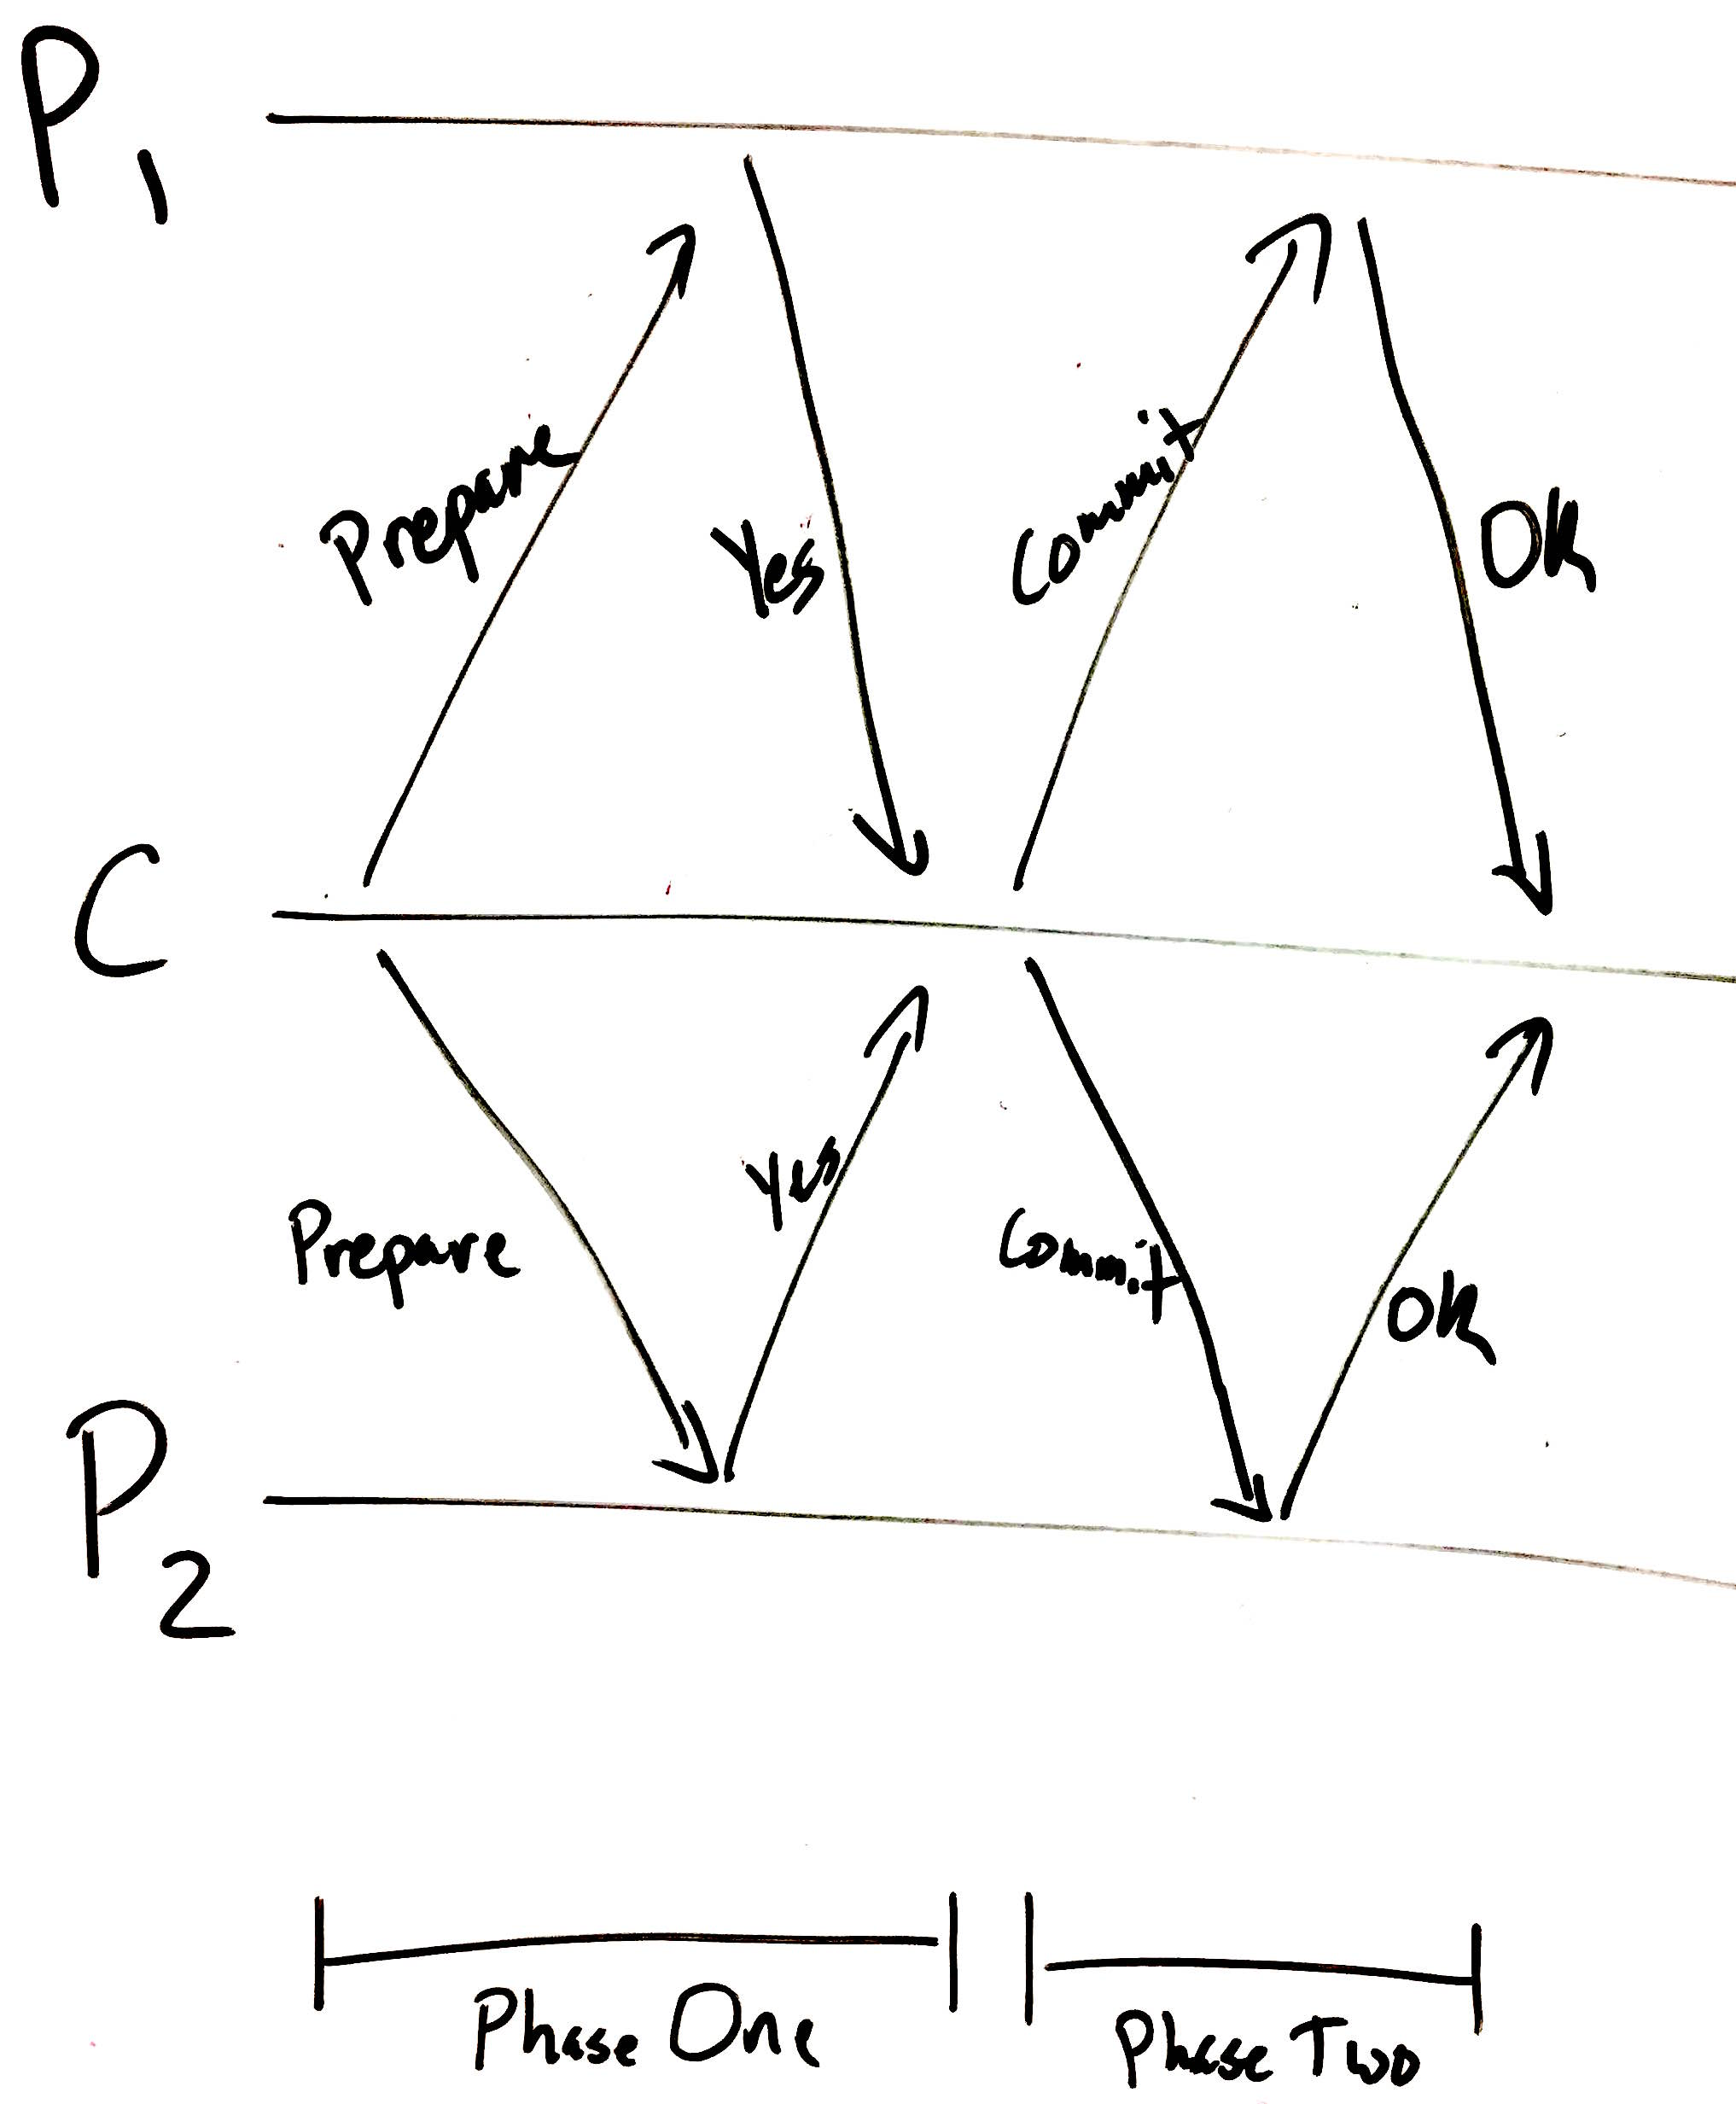
\includegraphics[width=0.96\textwidth]{tpc.pdf}
 \caption{One round of the Two-Phase Commit.}
  \label{fig:tpc-execution}
\end{minipage}
&
\begin{minipage}{0.55\linewidth}
\centering
\includegraphics[width=1.0\textwidth]{tpcstate.pdf}
\caption{States of a coordinator~(a) and a participant~(b).}
\label{fig:tpc-state}
\end{minipage}
\end{tabular}
\end{figure}
}




The Two-Phase Commit protocol designates a single node as the
\emph{coordinator}, which is in charge of managing the commit process;
other nodes participating in the protocol are \emph{participants}.
%
The protocol proceeds in a series of rounds, each of which makes a
single decision.
%
Each round consists of two phases; an example round execution is
shown in Fig.~\ref{fig:tpc-execution}.
%
In phase one, the coordinator begins processing a new transaction by sending
$\tprep$ messages to all participants.
%
Each participant responds with its local decision $\tyes$ or $\tno$.
%
In the figure, both participants vote $\tyes$, so the coordinator
enters phase two by sending $\tcommit$ messages to all participants,
informing them of its decision to commit.
%
If some participant had voted $\tno$, the coordinator would instead
send $\tabort$ messages.
%
In either case, participants acknowledge the decision by sending
$\tackcommit$ or $\tackabort$ to the coordinator.
%
When the coordinator receives all acknowledgments, it knows that all
nodes have completed the transaction.

The component of the coherence predicate constraining the local state
\code{l} (expressed via Coq/Ssreflect predicate notation \code{[Pred l
  | ...]}) of each node \code{n} depending on its role, coordinator or
a participant, is defined as follows:

%\newpage

\begin{lstlisting}[basicstyle=\footnotesize\ttfamily]
Definition localCoh (n: nid) := [Pred l | 
  if n == cn then exists(r: round) (s: CState) (log: Log), l = st :-> (r, s) \+ lg :-> log
  else if n \in pts 
        then exists(r: round) (s: PState) (log: Log), l = st :-> (r, s) \+ lg :-> log else True].
\end{lstlisting}
%
%
According to the predicate \code{localCoh}, the local state of the
coordinator (\code{cn} is a parameter bound at the level of the
protocol description) consists of two globally defined locations,
\code{st} and \code{lg}, which together store a round number
\texttt{r}, a \emph{coordinator status} \texttt{s}, and a
\texttt{log}.
% 
The state of a participant (\code{n} $\in$ \code{pts}) is similar, except
that its status is a \emph{participant status}.
%
Finally, any node which is not the coordinator or a participant (\eg,
a node participating only in other protocols) may have an arbitrary
local state with respect to \code{TPC}.

The coordinator's status can be in any of the seven states shown in
shown in Fig.~\ref{fig:tpc-state}(a). 
%
Between rounds, the coordinator waits in the $\cinit$ state.
%
From the initial state, the coordinators enters the \textsf{CSentPrep}
phase and remains in it until all prepare-requests are sent, after
which it switches into the receiving state $\mathsf{CWaitPrepResp}~x$
for the data $x$. 
%
Upon receiving all response message to the prepare-requests, the
coordinator changes either to the commit-state or to the abort-state,
notifying all of the participants about the decision and collecting
the acknowledgements, eventually returning to the $\cinit$ state with
an updated log.
%
The participants follow a similar pattern to the coordinators's,
except that a participant sends messages to or receives messages only
from the coordinator before changing its state.

{
\begin{figure}[t!]
\setlength{\belowcaptionskip}{-10pt}
{\centering
\begin{tabular}{c@{\ }c}
\begin{minipage}{0.5\linewidth}
\begin{lstlisting}[basicstyle=\scriptsize\ttfamily]
Definition c_send_step (r: round) (cs: CState) 
           (log: Log) (to: node) := match cs with
  (* Sending prepare-messages *)
  | CSentPrep x tos => if (* sent all messages *)
        (* switch for receiving responses *)
        then (r, CWaitPrepResp x [::], l)
        (* keep sending requests *)
        else (r, CSentPrep x (to :: tos), l)                  
  (* ...more cases depending on cs and to... *) 
  end.



\end{lstlisting}   
\end{minipage}
&
\begin{minipage}{0.5\linewidth}
\begin{lstlisting}[basicstyle=\scriptsize\ttfamily]
Definition c_recv_step (r : round) (cs : CState)
       (log : Log) (tag : nat) (mbody : seq nat) :=
  match cs with
  (* Waiting for prepare-responses *)
  | CWaitPrepResp x => if (* received all votes *)
      then (r, if (* all votes yes *)
                then CCommit x
	             else CAbort x, log)
      else (r, CWaitPrepResp, log)
  (* ...more cases depending on cs, tag, mbody... *)
  end.
\end{lstlisting}    
\vspace{-8pt}
\end{minipage}
\end{tabular}
}
\caption{Send and receive transitions of a coordinator in a \disel
  definition of the {\small\texttt{{TPC}}} protocol.}
\label{fig:coordinator-trans}
\end{figure}
}

Fig.~\ref{fig:coordinator-trans} shows how to encode a few of the
coordinator's transitions.
%
Recall that \disel transitions are computable functions that describe
how to update the local state of the node when executing the
transition.
%
The figure shows the snippets of \disel code related to sending a
prepare-request messages and receiving a corresponding response
message from participants.
%
In the latter case, depending on the responses, once all of them are
collected, the coordinator switches to either \textsf{CCommit} or
\textsf{CAbort} state.


\subsection{Program Specification and Implementation}
\label{sec:tpc-impl}

With the protocol in hand, we can now proceed to build programs that
implement the coordinator and participant and assign them useful
Hoare-style specifications.
%
An implementation of a single round of the coordinator and its Hoare
type are shown in Fig.~\ref{fig:tpc-ccode}.
%
The function \code{coordinator_round} takes as an argument the
transaction data to be processed in this round.
%
The type \code{\{r\ log\} DHT [cn, TPC] (...)} represents a Hoare
spec, whose logical variables are \code{r} and \code{log}. The spec is
parametrized by the dedicated coordinator node id \code{cn} and a
world with a single protocol instance \code{TPC}, with no hooks.
% 
The pre/postconditions (in parentheses) are encoded as Coq functions
\code{fun s => ...} and \code{fun res s' => ...}, correspondingly, so
the immediate pre/post-states \code{s}/\code{s'} are made explicit,
similarly to using the connective $\This{\mathsf{s}}$.

The precondition, which makes use of the \emph{local state getter}
\code{loc cn s = ...}, equivalent to the connective
$\mathsf{cn} \ppts{\mathtt{TPC}} \ldots$ from Fig.~\ref{fig:dsem},
requires that the coordinator is in the $\cinit$ state, with an
arbitrary round number and log.
%
The postcondition ensures that the local state has returned to
$\cinit$, the round number has been incremented, and the return value
accurately reflects the decision made on the data, which is also
reflected in the updated log.
%
The code proceeds along the lines required by the protocol: it reads
the round number from the local state, sends requests, collects the
responses and then, depending on the locally stored result~\texttt{b},
sends commit/abort messages, collecting the acknowledgements from
participants.

\subsection{Protocol Consistency and Inductive Invariant}
\label{sec:cons-induct-invar}

The spec given to \code{coordinator_round} in Fig.~\ref{fig:tpc-ccode}
only constrains the local state \code{loc} of the coordinator, but
in fact the protocol maintains stronger global invariants.
%
For example, we might like to conclude that between rounds, all logs
are in agreement.
%
This strong global agreement property is not implied by the coherence
predicate given above, so we must prove an inductive invariant that
implies it.
%
Finding such inductive invariants is the art of verification, and the
process typically requires several iterations before converging on a
property that is inductive and implies the desired spec.
%
Tools such as Ivy~\cite{Padon-al:PLDI16} make the process of finding
an inductive invariant much more pleasant by providing automatic
assistance in debugging and correcting invariants, and it would be
interesting to connect \disel to Ivy, which we leave to the future work.

{
\setlength{\belowcaptionskip}{-10pt} 
\begin{figure}
\centering
\begin{tabular}{@{\!\!}c@{\ }c} 
\begin{minipage}{0.5\linewidth}
\begin{lstlisting}[basicstyle=\scriptsize\ttfamily]
Definition coordinator_round (d : data) : 
{r log}, DHT [cn, TPC]
(fun s => loc cn s = st :-> (r, CInit) \+ lg :-> log,
 fun res s' => 
 loc cn s' = st:->(r+1, CInit) \+ lg:->(log++[(res, d)])) 
  := Do (r <-- read_round;
         send_prep_loop r d;;
         res <-- receive_prep_loop r;
         b <-- read_resp_result;
         (if b then send_commits r d;; 
                     receive_commit_loop r
                else send_aborts r d;; 
                     receive_abort_loop r);;
           return b).
\end{lstlisting}   
\vspace{-10pt}
\caption{Spec and code of a coordinator round.}
\label{fig:tpc-ccode}
\end{minipage}
&
\setlength{\belowcaptionskip}{-10pt} 
\begin{minipage}{0.5\linewidth}
\begin{lstlisting}[basicstyle=\scriptsize\ttfamily]
Definition run_coordinator (data_seq : seq data) :  
DHT [cn, _]  
(fun s => s = loc cn s = st :-> (0, CInit) \+ lg :-> [::]
 fun _ s' => exists (choices : seq bool),
   let r  := size data_seq in
   let lg := zip choices data_seq in
   loc cn s' = st :-> (r, CInit) \+ lg :-> log /\
   forall pt, pt \in pts -> 
         loc pt s' = st :-> (r, PInit) \+ lg :-> log)
 := Do (with_inv TPCInv (coordinator data_seq)).
\end{lstlisting}
\vspace{25pt} 
\caption{Coordinator spec elaborated with {\small\texttt{{TPCInv}}}.}
\label{fig:tpc-with-inv}    
\end{minipage}
\end{tabular}
\end{figure}
}



% \begin{figure}[t]
% {\centering
% \begin{lstlisting}[basicstyle=\footnotesize\ttfamily]
% Definition pt_PhaseTwoCommit cn pt r x log ms :=
% (loc pt = st :-> (r, PRespYes x) \+ lg :-> log
%  /\$ $ msg_spec cn pt commit_req [r] ms 
%  /\$ $ no_msg_from_to pt cn ms) \/
% (loc pt = st:-> (r, PCommitted x) \+$\!$ lg :-> (log++[(true, x)]) 
%  /\$ $ no_msg_from_to cn pt ms 
%  /\$ $ no_msg_from_to pt cn ms) \/
% (st :-> (r + 1, PInit) \+ lg :-> (log ++ [(true, x)])
%  /\$ $ no_msg_from_to cn pt ms
%  /\$ $ msg_spec pt cn commit_ack [r] ms).
% \end{lstlisting}
% }
% \caption{Part of the inductive invariant for a participant \texttt{pt}, describing the second phase after \texttt{pt} agreed to commit.}
% \label{fig:tpc-inv}
% \end{figure}

In this case, an invariant that closely follows the intuitive
execution of the protocol (its formulation can be found in our Coq
files) suffices to prove the global log agreement property.
%
For example, when the coordinator is in the $\csendcommit$ state, the
invariant ensures that all participants are either waiting to hear
about the decision, have received the decision but not acknowledged
it, or have acknowledged the decision and returned to the initial state.
%
The invariant also implies a simple statement of \emph{global log agreement},
shown below:
%
\begin{lstlisting}[basicstyle=\footnotesize\ttfamily]
Lemma cn_log_agreement d r log pt : loc cn d = st :-> (r, CInit) \+ lg :-> log -> 
        coh d -> TPCInv d -> forall pt, pt \in pts -> loc pt d = st :-> (r, PInit) \+ lg :-> log.
\end{lstlisting}
%  
In other words, a coordinator \code{cn} in the $\cinit$ state and a
round \code{r} can conclude that \emph{all} participants
{\small{$\mathtt{pt} \in \mathtt{pts}$}} have also reached the current
round \code{r} and have logs equal to its own.

\paragraph{Putting the inductive invariant to work.~}

We can freely use the elaborated invariant in proofs of programs.
%
Fig.~\ref{fig:tpc-with-inv} shows a coordinator program that executes
a series of rounds based on a given list \code{data_seq} of data
elements.
%
Its postcondition asserts that all participants have finished the
round and have logs agreeing with the one of the coordinator.
%
The proof of this specification is by a straightforward application of
the \textsc{WithInv} rule, making use of the elaborated invariant
\code{TPCInv} as well as the lemma \code{cn_log_agreement}.
%
Importantly, the postcondition is stable, because each round of the
Two-Phase Commit begins with a coordinator's move, hence no
participant can change its state from the ``initial'' one while the
coordinator's status is~$\cinit$.

\subsection{Composing Two-Phase Commit with a Querying Application
  using Hooks}
\label{sec:composing-two-phase}

 
Even though core consensus protocols, such as \code{TPC}, are not
designed to exist in isolation, but rather to be used in a context of
larger applications (\eg, for crash recovery), formal reasoning about
\emph{client-specific properties} (\ie, properties of applications
relying on certain characteristics of a ``core'' distributed protocol) is only
barely covered in classical textbooks~\cite{Weikum-Vossen:TIS02} and,
with a rare exception~\cite{Lesani-al:POPL16}, almost never a focus of
major verification
efforts~\cite{Woos-al:CPP16,Hawblitzel-al:SOSP15,rahli:eventml-avocs},
which, therefore cannot be reused in any larger verified context.

We now demonstrate how to employ \disel's logical mechanisms for
restricted composition of protocols in order to prove, in a modular
fashion, properties of client code from a core protocol's invariants.
%
To do so, we verify a composite application, which uses \code{TPC} for
building a replicated log of data elements, and a \emph{side-channel
  protocol} for sending independent queries about the state of
\code{TPC} participants (\eg, for the purpose of implementing recovery
after a coordinator's failure).
%
Fig.~\ref{fig:cn-query} shows a program that first calls the
coordinator program \code{run_coordinator}, and then uses the side
protocol to query the local state of a participant \code{pt}, which
the program then returns as its final result \code{res}.  Ignoring the
\code{query_init} part in the pre/postcondition for now, notice that
the postcondition asserts that \code{res} is \emph{equal to} the pair
\code{d} (round, log) stored in the local state of the coordinator
(which did not crash this time)!
 
Establishing such validity of the query \wrt \code{TPC}-related state
is, however, not trivial at all, given how the querying protocol is
defined. The protocol \code{Query} is very similar to the calculator
from Section~\ref{sec:overview}: any node $n_1$ in it can send a
request to any other node $n_2$, to which $n_2$ may respond with
\emph{any} arbitrary message (the details of the formal protocol
definition can be found in our Coq code). This protocol definition is
intentionally made very weak: while it allows one to prove some
interesting inductive invariants (\eg, no request is answered twice),
it leaves all other interaction aspects for the final client to
specify. In particular, it \emph{does not} enforce any specific shape
of data being sent in a response to a request.

{
\setlength{\belowcaptionskip}{-10pt} 
\begin{figure}
\centering
\begin{tabular}{c@{\ }c}
\!\!\!\!
\begin{minipage}{0.5\linewidth}
\begin{lstlisting}[basicstyle=\scriptsize\ttfamily]
Program Definition run_and_query (ds : seq data) pt :
  {reqs resp}, DHT [cn, (TPC \+ Query, QHook)]
  (fun s => loc s = st :-> (0, CInit) \+ lg :-> [::] /\
             pt \in pts  $\aand$  query_init s],
   fun (res : nat * Log) s' => exists (chs : seq bool),
     let d := (size ds, zip chs ds) in
     loc s' = st :-> (d.1, CInit) \+ lg :-> d.2 /\
     query_init s' $\aand$ res = d) 
  := Do (run_coordinator ds;;    
          rid <-- generate_fresh_request_id pt;
          send_request rid pt;;
          res <-- receive_responce rid pt;
          return res).
\end{lstlisting}   
\vspace{18pt}
\caption{Querying after the {\small\texttt{TPC}} coordinator.}
\label{fig:cn-query}
\end{minipage}
&
\begin{minipage}{0.5\linewidth}
\begin{lstlisting}[basicstyle=\scriptsize\ttfamily]
Parameter core_state : Data -> LocState -> Prop.
Parameter local_indicator : Data -> LocState -> Prop.

Definition QHook := (1, lab_c, lab_q, resp) :->
 fun lc lq m to => 
 forall rid data, m = rid :: serialize data -> 
               core_state data lc.

Hypothesis core_state_inj :
  forall l d d', core_state d l -> 
             core_state d' l -> d = d'.

Hypothesis core_state_step : forall data s s' n1 n2,
  n1 != n2 -> local_indicator data (loc lab_c n1 s) 
  -> network_step (lab_c :-> pc, $\emptyset$) n2 s s'
  -> core_state data (loc lab_c n2 s').
\end{lstlisting}
\vspace{-10pt}

\caption{Hook definition and abstract predicates.}
\label{fig:hook-ap}    
\end{minipage}
\end{tabular}
\end{figure}
}


Thus, without imposing the additional restriction that the protocol
\code{Query} \emph{can only transmit the local state of a node} \wrt
\code{TPC}, we will not be able to prove the spec in
Fig.~\ref{fig:cn-query}.
%
%This is where the mechanism of \disel's send-hooks comes to rescue.
%
The necessary restriction is provided by a send-hook entry
\code{QHook} that is used when composing the protocols \code{TPC} and
\code{Query} in the spec of \code{run_and_query}, and is defined in
Fig.~\ref{fig:hook-ap}.

In order to make the client verification effort reusable in the
context of \emph{any} consensus protocol, not just \code{TPC}, we
formulate the hook statement in terms of an abstract type \code{Data}
and an \emph{abstract predicate} \code{core_state}, which we will
later instantiate specifically for \code{TPC}, both afforded by Coq's
higher-order programming capabilities. The hook enforces that any
message \code{m} containing a request id \code{rid} and serialized
\code{data} adequately encodes the current local state (storing
\code{data}) of the sender node, at the moment of sending~\code{m},
with respect to the protocol with label \code{lab_c}.
%
The abstract predicate \code{core_state d lc}, capturing precisely
this ``adequacy of the encoding'', is supplied with the injectivity
hypothesis \code{core_state_inj} (to be proved by each consensus
implementation), which ensures that the abstract data representation
is unambiguous.

We also declare an abstract predicate \code{local_indicator} and the
corresponding hypothesis \code{core_state_step}, which essentially
corresponds to \emph{irrevocability} of consensus and should be proved
for each consensus implementation (in particular, for \code{TPC}),
ensuring that if a local state of a node \code{n1} is of certain shape
\code{data}, the local state of \code{n2}, captured by
\code{core_state data} will be remaining \emph{the same} under
interference (\code{network_step}) \wrt the core \code{lab_c}-labelled
protocol~\code{pc}---precisely what is ensured by the lemma
\code{cn_log_agreement} of~\code{TPC}.

Finally, we can use the abstract predicates from
Fig.~\ref{fig:hook-ap} to provide specifications for querying
procedures from Fig.~\ref{fig:cn-query}, stating \code{query_init} in
terms of assertions involving \code{local_indicator} and
\code{query_state}, in the context \emph{parameterized} over a
``core'' consensus protocol \code{pc} and restricted with
\code{QHook}.
%
To verify the program in Fig.~\ref{fig:cn-query} against the desired
spec we only need to instantiate the predicates as follows and prove
the corresponding hypotheses for \code{TPC}, which follow from the
invariant \code{TPCInv} and Lemma~\code{cn_log_agreement}:

\begin{lstlisting}[basicstyle=\footnotesize\ttfamily]
(* For TPC, abstract Data type is instantiated with a round number (nat) and Log. *)
Definition Data := nat * Log. 
Definition local_indicator (d : Data) l := l = st :-> (d.1, CInit) \+ log :-> d.2.
Definition core_state (d : Data) l        := l = st :-> (d.1, PInit) \+ log :-> d.2.
\end{lstlisting}
%
The rest of the proof is via the \Rule{Frame} rule with
$W = \angled{\text{\code{TPC}}, \emptyset}$, $C = \text{\code{Query}}$ and
$H = \text{\code{QHook}}$. Since \code{QHook} does not restrict the
transitions of \code{TPC}, $\NHooked$ holds.
%
Thanks to the parametrization of querying programs with abstract
predicates and hypotheses from Fig.~\ref{fig:hook-ap}, we can compose
them with any other instance of a consensus protocol, \eg,
Paxos~\cite{Lamport:TOPLAS98} or Raft~\cite{Ongaro-Ousterhout:UATC14},
thus, reusing the proofs of their core invariants.

% fig:hook-ap

% \todo{Outline the following things:}

% \begin{enumerate}

% \item Querying protocol (send/receive functions)'
% \item Imposed constraints
% \item Hook definition
% \item parameterization, abstract predicates and injectivity
% \item Final program
% \end{enumerate}

\section{Implementation and Experience}
\label{sec:eval-impl}

\disel combines two traits that rarely occur in a single tool for
reasoning about programs.  First, thanks to the representation of Hoare
types by means of Coq's dependent types, the soundness result of
\disel scales not just to a toy core calculus, but to the entirety of
Gallina, the \emph{programming language} of Coq, enhanced with general
recursion and message-passing primitives.
%
Second, \disel programs are immediately \emph{executable} by means of
extracting them into OCaml, which provides the features that Gallina
lacks: general fixpoints, mutable state, and networking constructs,
enabled by our trusted shim implementation.

% We briefly outline our experience of conducting mechanized proofs in
% \disel, and elaborate on some technical insights \wrt implementing an
% extraction mechanism for verified distributed programs with a minimal
% trusted code base.

\paragraph{Formal development and proof sizes.~}
% 
The size of our formalization of the metatheory, inference rules and
soundness proofs is about 4500 LOC.  Our development builds on
well-established {Ssreflect}/MathComp libraries
\cite{Gonthier-al:TR,Maboubi-Tassi:MathComp,Sergey:PnP} as well as on
the implementation of partial finite maps and heap theory
by~\citet{Nanevski-al:POPL10}.

%
\begin{wraptable}[21]{h}{0.54\textwidth}  
%\begin{table}[t]
\begin{minipage}{0.54\textwidth}
{
\sffamily\footnotesize 
% \centering
%\vspace{-12pt}
\begin{tabular}{|l|c|c|c|c|}
\hline
{Component} &  
{ {Defs/Specs}} & {{Impl}} & {{Proofs}} &
{Build}
\\ \hline \hline 
% \multicolumn{6}{|c|}{\textbf{Greeter}} \\\hline
% \emph{protocol} & 95& - & 40 & \multirow{2}{*}{2.5} & \multirow{2}{*}{$<$0.5\!}\\
% \textsf{hello\_world} &60 & 8 &78 & &  \\\hline
  \multicolumn{5}{|c|}{\textbf{Calculator} (\S\ref{sec:overview})} \\\hline
  \emph{protocol} (\S\ref{sec:calc-prot}) & \multirow{3}{*}{239} & 
        \multirow{3}{*}{-} & \multirow{3}{*}{243} &\multirow{3}{*}{4.8}  \\
  $\Inv_1$ (\S\ref{sec:elab-calc}) &&&& \\
  $\Inv_2$ (\S\ref{sec:more-impl-free}) &&&& \\\hline
  \textsf{$\osserver$} (\S\ref{sec:elab-calc}) & \multirow{3}{*}{192}
                & \multirow{3}{*}{43} & \multirow{3}{*}{153} & 
                                                               \multirow{3}{*}{8.6} \\
  \textsf{$\bserver$} (\S\ref{sec:more-impl-free}) &&&& \\
  \textsf{$\mserver$} (\S\ref{sec:more-impl-free}) &&&& \\\hline
  \textsf{$\cclient$} (\S\ref{sec:more-impl-free}) & 120 & 24 & 99 & 4.8 \\
  \textsf{$\dserver$} (\S\ref{sec:more-impl-free}) & 75 & 7 & 49 &2.4 \\\hline
  \multicolumn{5}{|c|}{\textbf{Two-Phase Commit}
  (\S\ref{sec:tpc-prot}--\S\ref{sec:cons-induct-invar})} 
  \\\hline
  \emph{protocol} (\S\ref{sec:tpc-prot}) & 465 & - & 231 & 3.9 \\\hline
  \textsf{coordinator} (\S\ref{sec:tpc-impl}) & 236  &  35  & 440 & 18 \\\hline
  \textsf{participant} (\S\ref{sec:tpc-impl}) & 163 & 24 & 198 & 10 \\\hline
  \texttt{\TPCInv} (\S\ref{sec:cons-induct-invar}) & 997 & - & 2113 & 25 \\\hline
  % 
  \multicolumn{5}{|c|}{\textbf{{Query}/{TPC}} (\S\ref{sec:composing-two-phase})} \\\hline
  \emph{protocol} & 169 & - & 115 & 2.1 \\\hline
  querying procedures & 326  &  18  & 707 & 19 \\\hline
  {\small\texttt{run\_and\_query}} & 76 & 5 & 89 & 2.6 \\
  % 
  [2pt]\hline
\end{tabular}
\vspace{5pt}
}
\end{minipage}
\caption{Statistics for implemented systems: sizes of protocol
  definitions/specs, programs, proofs of protocol
  axioms/invariants/specs (LOC), and build times (sec).  }
\label{tab:locs}
\end{wraptable}
%\end{table}
% 
Table~\ref{tab:locs} summarizes the proof effort for the calculator,
\code{TPC}/\code{Query} systems.
%
The \textsf{Defs/Specs} column measures all \emph{specification}
components, including, \eg, auxiliary predicates, whereas
\textsf{Impl} reports the sizes of actual \disel programs.
%
Due to the high degree of code reuse, it is difficult to provide
separate metrics in some cases; for those parts we only report the
joint numbers.
%
Although \disel is not yet a production-quality verification tool,
safety proofs of interesting systems can be obtained in it in a
reasonably short period of time and with moderate verification effort
(\eg, the full development of the core \code{TPC} system took nine
person-days of work).
%
Given that the current version of \disel employs no advanced proof
automation, beyond what is offered by Coq/Ssreflect, for discharging
program-level verification conditions~\cite{Chlipala:PLDI11} or
inductive invariant proofs~\cite{Padon-al:PLDI16}, we consider these
results encouraging for future development.

\paragraph{Extraction and execution.~}
\label{sec:extracting-runtime}

\disel's logic reasons about programs in terms of their denotational
semantics as traces, but each primitive also has a
straightforward operational meaning.
%
For example, executing a wrapped send transition should actually send
the corresponding network message.
%
Thus it is relatively straightforward to extract \disel programs by
providing OCaml implementations of the primitive operations in a
trusted shim.
%
Our shim consists of about 250 lines of OCaml, including primitives
for sending and receiving messages and general recursion.
%
The local state of each node is implemented as a map from protocol
labels to heaps, where a heap is implemented as a map from locations
to values.
%
Since \disel does not draw a distinction between real and auxiliary
state so far, both are manifested at run time.
%
In the future, we plan to allow users to mark state as auxiliary to
improve performance.
%
Due to artifacts of the extraction process, a \disel program that
appears tail-recursive at the Coq source level does not extract to a
tail-recursive OCaml program.
%
This causes long running loops (such as those typically used to
implement blocking receive) to quickly blow the OCaml stack.
%
To circumvent this issue, we added a while-loop combinator to \disel,
which is encoded using the general fixpoint combinator, but is extracted to
an efficient OCaml procedure that uses constant stack space.
%
Our implementations of the calculator and \code{TPC} use this
while-loop combinator to implement blocking receive.
%

In this work, our goal was not to extract high-performance code for
\disel programs, but rather show that, with a careful choice of
low-level primitives with precise operational meaning, such extraction
is feasible and requires a very small trusted codebase.
%
% We leave generation of fast distributed code (\eg, via
% staging~\cite{Romp:WF16}) for future work.

\paragraph{Adequacy of the extraction.~}

What is the correspondence between our denotational semantics,
presented in Section~\ref{sec:soundness} and the operational one
implemented by our shim? 
%
% Understanding this relation important in order to gain confidence in
% the resulting system.
%
While in this work we do not state a fully formal correspondence, as
the shim is written in OCaml and uses operating system and network
components, which have no formal semantics, we argue that the
extraction is adequate \wrt the denotational semantics for the
following reasons:
   
\begin{enumerate}

\item Our denotational semantics is simply a trace-collecting
  operational semantics for interleaved, asynchronous, message-passing
  concurrency, with the shared message soup being the only
  communication medium. Such an operational representation is widely
  considered adequate for modelling distributed systems and has been
  employed and evaluated (also, without verifying the extraction) in
  previous works~\cite{
    Wilcox-al:PLDI15,Hawblitzel-al:SOSP15,Padon-al:PLDI16}.

\item The shim implementation follows the operational rules from
  Fig.~\ref{fig:nsem} verbatim, and protocol transitions are encoded
  in \disel as \emph{functions} on the local state, so they are easy
  to extract and execute. The shim, thus, provides an accurate
  implementation of the protocol-aware network semantics.
 
\end{enumerate}

\noindent
%
Our fixpoint definition (available in our Coq sources) admits
non-terminating executions, ``approximating'' them iteratively by sets
of incomplete post-safe traces. It is extracted into OCaml's general
fixpoint operator, with a somewhat ad-hoc tail-call optimisation
described above in this Section. This means that our logic proves only
partial correctness: verified programs may loop at runtime, but they
will never violate the protocol.

\paragraph{Information hiding and separation.~}

One might wonder, whether we can \emph{hide} implementation-specific
parts of local state from the clients, \eg, when reasoning about other
nodes' implementations?
% 
At the moment any mutable state in \disel should be manifested
\emph{in a protocol definition} (and, thus, \emph{known} to all its
users) and can be only altered by sending/receiving. This is why in
the examples, such as the memoizing calculator from
Section~\ref{sec:more-impl-free}, we model hidden state by passing a
functional argument. However, what the framework \emph{does allow} one
to do is to encode an auxiliary protocol implementing a mutable
storage, which, once joined (via~$\uplus$) with its client protocol
(\eg, calculator), \emph{does not} have to be exposed to the clients
of the latter one, similarly to how it is done in the delegating
calculator example.

To support a version of a ``proper'' hidden local mutable state (\ie,
a heap with mutable pointers) we would need to formulate a nested
program logic with the corresponding low-level semantics for
state-manipulating programs---a direction we consider as interesting
future work, with an idea of adopting for this role Verifiable~C
by~\citet{Appel-al:BOOK14}.


\section{Related and Future Work}
\label{sec:related}

\subsection{Program Logics for Concurrency}

\disel builds on many ideas from modern program logics for
compositional concurrency reasoning.
%
The notion of protocols (often called \emph{regions}) in shared-memory
concurrency
logics~\cite{Turon-al:POPL13,DinsdaleYoung-al:ECOOP10,Nanevski-al:ESOP14,Turon-al:OOPSLA14,Raad-al:ESOP15,Svendsen-Birkedal:ESOP14}
provides a ``localized'' version of more traditional Rely/Guarantee
obligations~\cite{Jones:TOPLAS83}, which, in their original
formulation, are not
modular~\cite{Vafeiadis-Parkinson:CONCUR07,Feng:POPL09,Feng-al:ESOP07}.
%
The two closest to \disel logics employing protocols to reason about
interference are FCSL by~\citet{Nanevski-al:ESOP14} and GPS
by~\citet{Turon-al:OOPSLA14}. Besides those being logics for
\emph{shared-memory}, rather than \emph{message-passing} concurrency,
protocols in FCSL and GPS are tailored for the notion of
\emph{ownership transfer}~\cite{OHearn:TCS07}, as a way to express
exclusivity of access to shared resources.
%
Due to the lack of \emph{immediate} synchronization between nodes in a
message-passing setting, we consider the notion of ownership to be of
less use for most of the systems of interest. That said, even though
\disel does not feature explicit ownership transfer, it can be easily
encoded on a per-protocol basis, by defining a suitable local state
and transitions. 

Composition of modular proofs about protocols is a problem that has
not received much attention in modern concurrency logics. In FCSL,
which tackles a similar challenge, in order to constrain
inter-protocol interaction, a user must set up her protocols with a
very specific foresight of how they are going to be composed with
other protocols, defining \emph{intrinsic} ``ownership communication
channels'' for \emph{all} involved components, thus, effectively
prohibiting unforeseen interaction scenarios. This is not the case in
\disel: as we have shown in Section~\ref{sec:tpc}, ``core'' and
``client'' protocols (\eg, \code{TPC} and \code{Query}) can be
developed and verified independently and then composed in joint
applications via \emph{extrinsic} client-specified send-hooks.

The recent logical framework Iris~\cite{Jung-al:POPL15,Jung-al:ICFP16}
suggests to express protocols as a specific case of resources,
represented, in general, by partial commutative monoids, viewing
\emph{state reachability} as a specific instance of
\emph{framing}~\cite{Reynolds:LICS02}. This generality does not buy
much for verifying distributed applications, as the resulting proof
obligations are the same as when proving inductive invariants.  Having
an \emph{explicit} notion of protocols in the logic, though, allowed
us to provide the novel protocol-tailored rules \textsc{WithInv} and
\textsc{Frame} (\cf Fig.~\ref{fig:semass}), which enabled modular
invariant proofs and distributed systems composition.

A related logic by~\citet{Villard-al:APLAS09} only considers protocols
associated with specific message-passing channels, rather than entire
distributed systems.
%
% that is, not allowing one to make global
% assertions about a system's state, which is necessary to specify, \eg,
% consistency properties of \code{TPC}. 
%
In Villard~\etal's logic, messages do not carry any payload: they are
simply \emph{tags}, indicating ownership transfer of a certain heap
portion in the \emph{same} shared memory space. It is not immediately
obvious how to use Villard~\etal's specifications for \emph{locally}
asserting \emph{global} properties of stateful distributed systems
(e.g., the agreement of \code{TPC} in Fig.~\ref{fig:tpc-with-inv})
without considering all involved processes.
%
In addition to that, Villard~\etal's logic does not provide a
mechanism for establishing inductive contract invariants.
%
A recent framework \emph{Actor Services}
by~\citet{Summers-Muller:ESOP16} provides abstractions similar to our
protocol transitions, but only allows to state \emph{local} actor
invariants, and lacks a formal metatheory and soundness proof.
%

To the best of our knowledge, none of the existing concurrency logics
features \emph{both} foundational soundness proof (\ie, the proof that
the entire logic, not just its toy subset, is sound as a verification
tool), \emph{and} a mechanism to extract and run verified
applications.
%
% Furthermore, from the state-of-the art concurrency logics, only
% FCSL~\cite{Nanevski-al:ESOP14}, GPS~\cite{Turon-al:OOPSLA14} and
% Iris~\cite{Jung-al:POPL15} come with the foundational mechanized
% proofs of soundness, but those are logics for \emph{shared-memory}
% concurrency, rather than for message-passing distributed
% systems. Encoding the distributed message-based communication with the
% corresponding notion of distributed state, principles of modular
% reasoning and protocol composition in those logics, even if possible,
% is not trivial and has not been done yet.

\subsection{Types for Distributed Systems}
%
% A number of type systems have been proposed for distributed programs
% to enforce race-freedom and local state
% invariants~\cite{Kloos-al:ECOOP15}, ownership
% transfer~\cite{Haller-Odersky:ECOOP10},
% immutability~\cite{Liblit-Aiken:POPL00,Gordon-al:OOPSLA12}
% disciplines.
%
Session Types~\cite{Honda-al:ESOP98} are traditionally used to ensure
that distributed parties follow a predefined communication protocol
\wrt a specific channel. While the
\emph{multiparty}~\cite{Honda-al:POPL08} and
\emph{multirole}~\cite{Denielou-Yoshida:POPL11} Session Types enable a
form of system composition and role-play, and \emph{dependent session
  types} allow one to quantify over messages~\cite{Toninho-al:PPDP11},
session types do not allow quantification over the global system state
and reasoning out of inductive invariants, neither do they allow
restricted composition of protocols.

We believe that \disel's combination of Hoare types and protocols
provides the necessary level of expressivity to capture rich safety
properties of distributed applications.
%
A similar approach has been explored in $\fstar$
by~\citet{Swamy-al:ICFP11}, although that work did not reason about
inductive invariants separately from implementations, neither did it
address composition of systems with inter-protocol dependencies.

\subsection{Verification of Large Systems}

Recent work has verified implementations of core pieces of distributed
systems infrastructure, both by using specialized models and DSLs.


IronFleet~\cite{Hawblitzel-al:SOSP15} supports proving \emph{liveness}
in addition to safety, all embedded in Dafny~\cite{Leino:LPAR10}.
%
% Its Hoare logic fragment is \emph{local} and does not allow to
% quantify over global system state. 
%
IronFleet focuses on layered verification of standalone monolithic
systems. 
%
In those systems, each layer is a state-transition system (STS)
specifying the system's behavior at a certain abstraction level, with
the top-most layer expressing how a collection of nodes together
implement a high-level (\eg, shared-memory) specification,
%
and the actual implementation, run by the nodes, at the bottom.
%
Adjacent layers are connected by establishing refinement between
their %
STSs via reduction~\cite{Lipton-CACM75}, which often involves proving
inductive invariants, similar to what we have proven in \disel.
%
% IronFleet's specifications in the form of abstract STSs hide
% complexity of distributed interaction in a system, allowing the
% clients to reason about the system's properties.
%
In our understanding, such specifications do not allow for horizontal
composition, \ie, reasoning about interaction with separately verified
systems in a client code. 
%
Such an interaction has been, however, explored \wrt
\emph{shared-memory} concurrency by~\citet{Gu-al:OSDI16}, who built a
series of abstraction layers in a verified concurrent OS kernel. That
work has shown that establishing a refinement between a spec STSs and
a \emph{family} of interacting lower-level STSs is possible, although
the proofs are usually quite complex, as they involve reasoning about
\emph{semantics} of a restricted product of STSs.
%
In contrast with those systems, \disel's logic does not provide
machinery to establish STS refinement, but rather explicitly
identifies valid linearization points~\cite{Herlihy-Wing:TOPLAS90} in
the implementations, as they correspond precisely to taken protocol
transitions.
%
Abstract specifications and the corresponding system properties, usable
by client code, such as consensus, are encoded in \disel via
parametrized Hoare types and abstract predicates, as shown in
Section~\ref{sec:composing-two-phase}.

Verdi~\cite{Wilcox-al:PLDI15, Woos-al:CPP16} provides a form of
\emph{vertical compositionality} by means of verified system
transformers, which allow systems to be decomposed into layers of
functionality (\eg, sequence numbers or state machine replication).
%
The Chapar framework by~\citet{Lesani-al:POPL16} is tailored to
causally consistent key-value stores, and also provides verified model
checking for client programs using the verified KV stores.
%
Ivy is a tool to assist users in iteratively discovering inductive
invariants by finding counterexamples to
induction~\cite{Padon-al:PLDI16}.
%
\textsc{PSync} by~\citet{Dragoi-al:POPL16} is a DSL allowing one to
prove inductive invariants of consensus algorithms in networks with
potential faults, operating in a synchronous round-based
model~\cite{Elrad-Frances:SCP82}. This assumption enables efficient
proof automation, but prohibits low-level optimizations, such as, \eg,
batching.
%
Mace by~\citet{Killian-al:PLDI07} and DistAlgo
by~\citet{Liu-al:OOPSLA12} adopt an asynchronous protocol model,
similar to ours.
%
Mace provides a suite of tools for generating and model checking
distributed systems, while DistAlgo allows extraction of efficient
implementation from a high-level protocol description.
%
EventML is another DSL for verifying monolithic distributed systems,
based on compiling to the Logic of Events in
Nuprl~\cite{rahli:eventml-avocs}.
%
None of these frameworks tackles the challenges of modular reasoning
about horizontally composed systems~\textbf{(2)} and elaborated
protocols~\textbf{(3)}, stated in the introduction of this paper.

Arguably, our Two-Phase Commit implementation is a relatively small
case study when compared to the systems verified in IronFleet, Verdi,
and EventML. Nevertheless, we are sure that, given enough time and
manpower, we can conduct safety proofs of
Raft~\cite{Ongaro-Ousterhout:UATC14} and
MultiPaxos~\cite{vanRenesse-Altinbuken:ACS15} in \disel, as their
implementations and invariants are based on the same semantic
primitives and reasoning principles that were employed for \code{TPC}.
%
We believe, though, that compositionality, afforded by \disel's
logical mechanisms, is a key to make the results of future
verification efforts reusable for building even larger verified
distributed ecosystems. 

\subsection{Future Work}

We consider \disel as just the beginning of our journey towards
building modularly verified and highly reusable distributed
implementations.
%
Our next steps are to investigate more protocol combinators, in
addition to \Rule{WithInv}, establishing refinement, in the spirit of
certified abstraction layers~\cite{Gu-al:OSDI16}, of the higher-level
distributed models (\eg,~round-based register
by~\cite{Boichat-al:SN03}) by current \disel's protocols, formulated
in terms of send/receive transitions.
%
We are also going to expand the language fragment for local node
implementations with more imperative features, such as exceptions and
concurrency.
%
We are planning to incorporate the ideas from program logics to
reason, in a modular way, about local system
faults~\cite{Ntzik-al:APLAS15} and liveness properties under fairness
assumptions~\cite{Liang-Feng:POPL16}.
%
Finally, we are going to investigate possibilities for automating
proofs of inductive
invariants~\cite{Padon-al:PLDI16,Padon-al:OOPSLA17}.

\vspace{-5pt}   

\section{Conclusion}
\label{sec:conclusion}

Almost two decades ago, \citet{Lamport:COMPOS97} propounded the thesis
\textbf{Composition: a way to make proofs harder}, favoring
mathematical models over program logics for real system verification:
%
``\emph{in 1997, the unfortunate reality is that engineers rarely
  specify and reason formally about the systems they
  build. \emph{[...]} It seems unlikely that reasoning about the
  composition of open-system specifications will be a practical
  concern within the next 15 years}''.
%
He was right: it took two decades of active research in rigorous
program verification, combining the strengths of mathematical models
(protocols) and program logics, to make compositional verification of
open-world systems today's reality.

\vspace{-5pt}

% \begin{acks}
%   We thank Philippa Gardner, Alexey Gotsman, Yoichi Hirai, Ranjit
%   Jhala, Luke Nelson, Karl Palmskog, Daniel Ricketts, Doug Woos, and
%   Nobuko Yoshida for their comments on earlier drafts of this paper.
%   %
%   We are grateful to the PLDI'17 reviewers, especially Reviewers~C
%   and~E, for their feedback regarding insufficient support for
%   modularity in an earlier version of \disel, which forced us to
%   revise the approach and introduce the notion of send-hooks.
%   %
%   We wish to acknowledge the feedback by the OOPSLA'17 reviewers on
%   the presentation.
%   % 
%   We thank the POPL'18 PC and AEC reviewers for the careful reading
%   and many constructive suggestions on the paper and the implementation.
%   %
%   Finally, we thank \'{E}ric Tanter for his dedication to bring out
%   the best of the paper as our shepherd, and Andrew C. Myers for his
%   efforts as POPL'18 PC chair.
% 
%   Sergey's research was supported by EPSRC First Grant EP/P009271/1
%   ``Program Logics for Compositional Specification and Verification of
%   Distributed Systems''. Tatlock's research was supported by a
%   generous gift from Google.
% %
%   This material is based upon work supported by the National Science
%   Foundation Graduate Research Fellowship under Grant No. DGE-1256082.
%   Any opinion, findings, and conclusions or recommendations expressed
%   in this material are those of the authors and do not necessarily
%   reflect the views of the National Science Foundation.
% \end{acks}


\chapter{\mypyvy}
\label{chap:mypyvy}

% Put this somewhere
%  % The project started because I wanted a clean sandbox in which
%  % to implement the \updr invariant inference algorithm~\cite{updr-jacm}.

\section{Introduction}

\begin{verbatim}
- something something invariant inference
- something something clean research platform
\end{verbatim}

\todo{delete}
\lipsum[1]

\section{Background on Transition Systems}

\subsection{The robot example informally and pictorially}

\def\xMin{-8}
\def\xMax{8}
\def\yMin{-5}
\def\yMax{11}

\begin{figure}[t]
  \hfil%
  \begin{minipage}{0.45\linewidth}
    \centering
    \begin{tikzpicture}[scale=0.35, >=stealth]
      \foreach \i in {\xMin,...,\xMax} {
          \draw [very thin,gray] (\i,\yMin) -- (\i,\yMax);
      }
      \foreach \i in {\yMin,...,\yMax} {
          \draw [very thin,gray] (\xMin,\i) -- (\xMax,\i);
      }
      \draw[<->, thick] (\xMin, 0) -- (\xMax, 0);
      \draw[<->, thick] (0, \yMin) -- (0, \yMax);
      \fill[fill=red, fill opacity=0.3] (0, 0) circle [radius=3];
      \draw[fill=black] (0, 5) circle [radius=0.25];
    \end{tikzpicture}
    \caption{Robot initial configuration.}
    \label{fig:robot-init}
  \end{minipage}%
  \hfil%
  \begin{minipage}{0.45\linewidth}
    \centering
    \begin{tikzpicture}[scale=0.35, >=stealth]
      \foreach \i in {\xMin,...,\xMax} {
          \draw [very thin,gray] (\i,\yMin) -- (\i,\yMax);
      }
      \foreach \i in {\yMin,...,\yMax} {
          \draw [very thin,gray] (\xMin,\i) -- (\xMax,\i);
      }
      \draw[<->, thick] (\xMin, 0) -- (\xMax, 0);
      \draw[<->, thick] (0, \yMin) -- (0, \yMax);
      \fill[fill=red, fill opacity=0.3] (0, 0) circle [radius=3];
      \draw[fill=black] (0, 5) circle [radius=0.25];
      \draw[->, line width=1.5pt] (0, 5) -- (0, 6);
      \draw[->, line width=1.5pt] (0, 5) -- (1, 4);
    \end{tikzpicture}
    \caption{Robot's first steps.}
    \label{fig:robot-first-steps}
  \end{minipage}%
  \hfil%
  \hrule
  \vspace{1em}
  \begin{minipage}{1\linewidth}
    \centering
    \begin{minipage}{0.5\linewidth}
      \centering
      \begin{tikzpicture}[scale=0.35, >=stealth]
        \foreach \i in {\xMin,...,\xMax} {
            \draw [very thin,gray] (\i,\yMin) -- (\i,\yMax);
        }
        \foreach \i in {\yMin,...,\yMax} {
            \draw [very thin,gray] (\xMin,\i) -- (\xMax,\i);
        }
        \draw[<->, thick] (\xMin, 0) -- (\xMax, 0);
        \draw[<->, thick] (0, \yMin) -- (0, \yMax);
        \fill[fill=red, fill opacity=0.3] (0, 0) circle [radius=3];
        \draw[fill=black] (0, 5) circle [radius=0.25];
        \draw[->, line width=1.5pt] (0, 5) -- (0, 6);
        \draw[->, line width=1.5pt] (0, 5) -- (1, 4);
        \draw[->, line width=1.5pt] (0, 6) -- (0, 7);
        \draw[->, line width=1.5pt] (0, 6) -- (1, 5);
        \draw[->, line width=1.5pt] (1, 4) -- (1, 5);
        \draw[->, line width=1.5pt] (1, 4) -- (2, 3);
      \end{tikzpicture}%
    \end{minipage}%
    \begin{minipage}{0.5\linewidth}
      \centering
      \begin{tikzpicture}[scale=0.35, >=stealth]
        \foreach \i in {\xMin,...,\xMax} {
            \draw [very thin,gray] (\i,\yMin) -- (\i,\yMax);
        }
        \foreach \i in {\yMin,...,\yMax} {
            \draw [very thin,gray] (\xMin,\i) -- (\xMax,\i);
        }
        \draw[<->, thick] (\xMin, 0) -- (\xMax, 0);
        \draw[<->, thick] (0, \yMin) -- (0, \yMax);
        \fill[fill=red, fill opacity=0.3] (0, 0) circle [radius=3];
        \draw[fill=black] (0, 5) circle [radius=0.25];
        \draw[->, line width=1.5pt] (0, 5) -- (0, 6);
        \draw[->, line width=1.5pt] (0, 5) -- (1, 4);
        \draw[->, line width=1.5pt] (0, 6) -- (0, 7);
        \draw[->, line width=1.5pt] (0, 6) -- (1, 5);
        \draw[->, line width=1.5pt] (1, 4) -- (1, 5);
        \draw[->, line width=1.5pt] (1, 4) -- (2, 3);
        \draw[->, line width=1.5pt] (0, 7) -- (0, 8);
        \draw[->, line width=1.5pt] (0, 7) -- (1, 6);
        \draw[->, line width=1.5pt] (1, 5) -- (1, 6);
        \draw[->, line width=1.5pt] (1, 5) -- (2, 4);
        \draw[->, line width=1.5pt] (2, 3) -- (2, 4);
        \draw[->, line width=1.5pt] (2, 3) -- (3, 2);
      \end{tikzpicture}
    \end{minipage}%
    \caption{Robot's second and third steps.}
    \label{fig:robot-23-steps}
  \end{minipage}
\end{figure}

Imagine robot in a 2-dimensional world.
The robot starts at position $(0, 5)$,
  and can take steps to integer grid points either
 due north or diagonally southeast of its current position.
The world has a circular hole of radius 3 centered at the origin.
Can the robot ever fall in the hole?\footnote{Thanks to Jon Howell for this example.}

The initial situation is depicted in \cref{fig:robot-init}.
The smaller black circle represents the robot's initial position,
  and the larger shaded red circle represents the hole at the origin.
In its first step, shown in \cref{fig:robot-first-steps},
  the robot could either move north one square,
  or diagonally southeast one square.
These two possibilities are drawn as thick black arrows.
So far, the robot manages to avoid falling in.

As the robot progresses, more and more positions are reachable,
  each with a sequence of moves due north or diagonally southeast.
The set of possible positions after two and three steps
  are shown in \cref{fig:robot-23-steps}.
Despite the growing number of reachable positions,
  no sequence of steps causes the robot to fall in.

\begin{figure}[t]
  \hfil%
  \begin{minipage}{0.45\linewidth}
    \centering
    \begin{tikzpicture}[scale=0.35, >=stealth]
      \foreach \i in {\xMin,...,\xMax} {
          \draw [very thin,gray] (\i,\yMin) -- (\i,\yMax);
      }
      \foreach \i in {\yMin,...,\yMax} {
          \draw [very thin,gray] (\xMin,\i) -- (\xMax,\i);
      }
      \draw[<->, thick] (\xMin, 0) -- (\xMax, 0);
      \draw[<->, thick] (0, \yMin) -- (0, \yMax);
      \fill[fill=red, fill opacity=0.3] (0, 0) circle [radius=3];
      \draw[fill=black] (0, 5) circle [radius=0.25];
      \fill[fill=green, fill opacity=0.3] (0, 5) -- (0, \yMax) -- (\xMax, \yMax) -- ($(\xMax,5)-(0,\xMax)$) -- cycle;
    \end{tikzpicture}
    \caption{Exact characterization of the robot's reachable positions.}
    \label{fig:robot-reachable}
  \end{minipage}%
  \hfil%
  \begin{minipage}{0.45\linewidth}
    \centering
    \begin{tikzpicture}[scale=0.35, >=stealth]
      \foreach \i in {\xMin,...,\xMax} {
          \draw [very thin,gray] (\i,\yMin) -- (\i,\yMax);
      }
      \foreach \i in {\yMin,...,\yMax} {
          \draw [very thin,gray] (\xMin,\i) -- (\xMax,\i);
      }
      \draw[<->, thick] (\xMin, 0) -- (\xMax, 0);
      \draw[<->, thick] (0, \yMin) -- (0, \yMax);
      \fill[fill=red, fill opacity=0.3] (0, 0) circle [radius=3];
      \draw[fill=black] (0, 5) circle [radius=0.25];
      \fill[fill=blue, fill opacity=0.3] (0, 5) -- ($(-\yMax,\yMax)+(5,0)$) -- (\xMax, \yMax) -- ($(\xMax,5)-(0,\xMax)$) -- cycle;
    \end{tikzpicture}
    \caption{A simple overapproximation to the set of reachable positions.}
    \label{fig:robot-inductive-invariant}
  \end{minipage}
  \hfil%
\end{figure}

We start to see a pattern emerging.
No matter what happens,
  the robot will never be able to move west of the $y$ axis,
  nor will it be able to move southwest
    of the diagonal line $x + y = 5$.
This region is shown shaded in green in \cref{fig:robot-reachable}.
Visually, this green polygonal region does not overlap with the red circle,
  which ``proves'' that the robot never falls in.

In fact, this green region exactly characterizes
  the set of possible positions that the robot could reach
  through some sequence of moves.
(We call such positions ``reachable''.)
Given any point in the green region,
  the robot can reach it by first moving southeast over and over until
  it is vertically below the target point,
  and then moving due north over and over until the point is reached.

Our proof that the robot never falls in
  can be simplified slightly be noticing
  that we never used the fact that
  the robot always remains east of the $y$ axis.
Instead, it is enough to convince ourselves that
  the robot is always northeast of the line $x + y = 5$.
This region is shown in blue in \cref{fig:robot-inductive-invariant}.
Again, it does not visually overlap with the circle,
  so it constitutes a visual ``proof'' that the robot never falls in.

This time, though, not every position in the blue polygonal region is reachable,
  since we have already realized that no position west of the $y$ axis is reachable.
The unreachable positions from this region are shown in \cref{fig:robot-unreachable}.
This second proof demonstrates that we can prove the robot never falls in
  even without exactly characterizing the set of reachable positions.

\begin{figure}[t]%
%  \centering%
  \hfil%
  \begin{minipage}{0.45\linewidth}
    \centering
    \begin{tikzpicture}[scale=0.35, >=stealth]
      \foreach \i in {\xMin,...,\xMax} {
          \draw [very thin,gray] (\i,\yMin) -- (\i,\yMax);
      }
      \foreach \i in {\yMin,...,\yMax} {
          \draw [very thin,gray] (\xMin,\i) -- (\xMax,\i);
      }
      \draw[<->, thick] (\xMin, 0) -- (\xMax, 0);
      \draw[<->, thick] (0, \yMin) -- (0, \yMax);
      \fill[fill=red, fill opacity=0.3] (0, 0) circle [radius=3];
      \draw[fill=black] (0, 5) circle [radius=0.25];
      \fill[fill=yellow, fill opacity=0.3] (-1, 5) -- (-1, \yMax) -- ($(-\yMax,\yMax)+(5,0)$) -- cycle;
    \end{tikzpicture}
    \caption{Positions from \cref{fig:robot-inductive-invariant} that are unreachable.}
    \label{fig:robot-unreachable}
  \end{minipage}%
  \hfil%
  \begin{minipage}{0.45\linewidth}
    \centering
    \begin{tikzpicture}[scale=0.35, >=stealth]
      \foreach \i in {\xMin,...,\xMax} {
          \draw [very thin,gray] (\i,\yMin) -- (\i,\yMax);
      }
      \foreach \i in {\yMin,...,\yMax} {
          \draw [very thin,gray] (\xMin,\i) -- (\xMax,\i);
      }
      \draw[<->, thick] (\xMin, 0) -- (\xMax, 0);
      \draw[<->, thick] (0, \yMin) -- (0, \yMax);
      \fill[fill=red, fill opacity=0.3] (0, 0) circle [radius=3];
      \draw[fill=black] (0, 5) circle [radius=0.25];
      \fill[fill=orange, fill opacity=0.3]
      (\xMin, -\xMin) -- (\xMin, \yMax) -- (\xMax, \yMax) -- (\xMax, \yMin) --
      (-\yMin, \yMin) -- cycle;
      \draw[red,fill=red] (1, 1) circle [radius=0.25];
    \end{tikzpicture}
    \caption{The orange region is unsafe because it intersects the red circle.}
    \label{fig:robot-unsafe}
  \end{minipage}%
%  \dotfill
  \hfil
\end{figure}

\begin{figure}[t]
  \centering
\end{figure}

Reflecting on our two admittedly informal proofs so far,
  we can boil them each down into three essential proof steps:
  (1) identify a set of positions $I$ that
  (2) contains all reachable positions; and that
  (3) does not intersect the red circle.
Each proof step is important.
Proof step (1) requires some creativity and foresight
  to pick a set that will make proof steps (2) and (3) possible.
Proof step (3) has been fairly straightforward so far,
  because we can visually analyze our set and the red circle
  to determine if they overlap.
If we wanted to be more precise about proof step (3),
  we could do some algebra to show that
  any position $(x, y)$ that satisfies the linear inequalities
  that define the polygonal regions from
    \cref{fig:robot-reachable,fig:robot-inductive-invariant}
  always fall outside the red circle,
  i.e. $\sqrt{x^2 + y^2} > 3$.

Proof step (2) is more subtle.
We have claimed informally that the robot will never
  be able to move southwest of the line $x + y = 5$,
  nor west of the $y$ axis,
  but what would constitute a more detailed proof of this fact?
These claims are claims of \emph{invariance},
  i.e., that the set $I$ from proof step (1) is an invariant,
  where an invariant is a set that contains all reachable positions.
The key to proving invariance is an \emph{inductive} argument,
  which first shows (2.1) that the initial position is in $I$
  and then shows (2.2) that, from any position in $I$,
  all steps the robot could take
  lead to new positions that are also in $I$.
By induction, this implies that all reachable positions
  are contained in $I$.
For the invariants represented in
  \cref{fig:robot-reachable,fig:robot-inductive-invariant}
  we could make proof steps (2.1) and (2.2) more precise
  by showing that the initial position
    satisfies the linear inequalities for the polygonal regions
  and by showing that if $(x,y)$ satisfies the inequalities,
    then so do both $(x, y+1)$ (moving due north)
      and $(x+1, y-1)$ (moving southeast).

\begin{figure}[t]%
%  \centering%
  \hfil%
  \begin{minipage}{0.45\linewidth}
    \centering
      \begin{tikzpicture}[scale=0.35, >=stealth]
        \foreach \i in {\xMin,...,\xMax} {
            \draw [very thin,gray] (\i,\yMin) -- (\i,\yMax);
        }
        \foreach \i in {\yMin,...,\yMax} {
            \draw [very thin,gray] (\xMin,\i) -- (\xMax,\i);
        }
        \draw[<->, thick] (\xMin, 0) -- (\xMax, 0);
        \draw[<->, thick] (0, \yMin) -- (0, \yMax);
        \fill[fill=red, fill opacity=0.3] (0, 0) circle [radius=3];
        \draw[fill=black] (0, 5) circle [radius=0.25];
        \draw[red, ->, line width=1.5pt] (-2, 3) -- +(1, -1);
        \draw[red, ->, line width=1.5pt] (1, -3) -- +(0, 1);
        \fill[even odd rule, fill=orange, fill opacity=0.3]
        (0, 4) -- ++(1, -1) -- ++(1, 0) -- ++(1, -1) -- ++(0, -1) -- ++(1, -1)
               -- ++(-1, -1) -- ++(0, -1) -- ++(-1, -1) -- ++(-1, 0) -- ++(-1, -1)
               -- ++(-1, 1) -- ++(-1, 0) -- ++(-1, 1) -- ++(0, 1) -- ++(-1, 1)
               -- ++(1, 1) -- ++(0, 1) -- ++(1, 1) -- ++(1, 0) -- ++(1, 1)
               -- cycle
        (\xMin, \yMax) -- (\xMax, \yMax) -- (\xMax, \yMin) -- (\xMin, \yMin) -- cycle;
      \end{tikzpicture}
    \caption{The region outside the circle is invariant but not inductive.}
    \label{fig:robot-cti1}
  \end{minipage}%
  \hfil%
  \begin{minipage}{0.45\linewidth}
    \centering
    \begin{tikzpicture}[scale=0.35, >=stealth]
      \foreach \i in {\xMin,...,\xMax} {
          \draw [very thin,gray] (\i,\yMin) -- (\i,\yMax);
      }
      \foreach \i in {\yMin,...,\yMax} {
          \draw [very thin,gray] (\xMin,\i) -- (\xMax,\i);
      }
      \draw[<->, thick] (\xMin, 0) -- (\xMax, 0);
      \draw[<->, thick] (0, \yMin) -- (0, \yMax);
      \fill[fill=red, fill opacity=0.3] (0, 0) circle [radius=3];
      \draw[fill=black] (0, 5) circle [radius=0.25];
      \fill[even odd rule, fill=orange, fill opacity=0.3]
      (0, 5) -- (5, 0) -- (5, -4) -- (-5, -4) -- (-5, 5) -- cycle
      (\xMin, \yMax) -- (\xMax, \yMax) -- (\xMax, \yMin) -- (\xMin, \yMin) -- cycle;
      \draw[red, ->, line width=1.5pt] (-5, 5) -- (-4, 4);
      \draw[red, ->, line width=1.5pt] (2, -4) -- +(0, 1);
    \end{tikzpicture}
    \caption{This simplified region is also invariant but not inductive.}
    \label{fig:robot-cti2}
  \end{minipage}%
%  \dotfill
  \hfil
\end{figure}

It is instructive to see what happens when
  the set $I$ selected in proof step (1)
  fails to proof steps (2) or (3).
When proof step (3) fails,
  $I$ intersects the red circle,
  as in \cref{fig:robot-unsafe}.
In this case we call the set $I$ ``unsafe''.
The small opaque red dot shows an example position that is both
  in the candidate set $I$ drawn as the orange region
  and the shaded red circle at the origin.
When proof step (2) fails,
  there is a position in $I$ from which
  the robot can step to a position outside $I$,
  as in \cref{fig:robot-cti1,fig:robot-cti2}.
The red arrows show examples of positions in the orange regions
  that can step out of orange regions.
We call such positions ``counterexamples to inductiveness'', or CTIs.

\begin{figure}[t]%
  \hfil%
  \begin{minipage}{0.45\linewidth}
    \centering
    \begin{tikzpicture}[scale=0.35, >=stealth]
      \foreach \i in {\xMin,...,\xMax} {
          \draw [very thin,gray] (\i,\yMin) -- (\i,\yMax);
      }
      \foreach \i in {\yMin,...,\yMax} {
          \draw [very thin,gray] (\xMin,\i) -- (\xMax,\i);
      }
      \draw[<->, thick] (\xMin, 0) -- (\xMax, 0);
      \draw[<->, thick] (0, \yMin) -- (0, \yMax);
      \fill[fill=red, fill opacity=0.3] (0, 0) circle [radius=3];
      \draw[fill=black] (0, 5) circle [radius=0.25];
      \fill[fill=violet, fill opacity=0.4] (0, 5) -- (3, 2) -- (3, 1) -- (4, 0) -- (4, \yMin) -- (\xMax, \yMin) -- (\xMax, \yMax) -- ($(-\yMax,\yMax)+(5,0)$) -- cycle;
    \end{tikzpicture}
    \caption{The largest safe inductive invariant for the robot.}
    \label{fig:robot-large-invariant}
  \end{minipage}%
  \hfil%
  \begin{minipage}{0.45\linewidth}
    \centering
    \begin{tikzpicture}[scale=0.35, >=stealth]
      \foreach \i in {\xMin,...,\xMax} {
          \draw [very thin,gray] (\i,\yMin) -- (\i,\yMax);
      }
      \foreach \i in {\yMin,...,\yMax} {
          \draw [very thin,gray] (\xMin,\i) -- (\xMax,\i);
      }
      \draw[<->, thick] (\xMin, 0) -- (\xMax, 0);
      \draw[<->, thick] (0, \yMin) -- (0, \yMax);
      \fill[fill=red, fill opacity=0.3] (0, 0) circle [radius=3];
      \draw[fill=black] (0, 5) circle [radius=0.25];
      \fill[fill=violet, fill opacity=0.4] (0, 5) -- (3, 2) -- (3, 1) -- (4, 0) -- (4, \yMin) -- (\xMax, \yMin) -- (\xMax, \yMax) -- ($(-\yMax,\yMax)+(5,0)$) -- cycle;
      \draw[->, red, line width=1.5pt] ($(-\yMax,\yMax)+(4,0)$) -- (2, 2);
      \draw[->, red, line width=1.5pt] (3, \yMin) -- (3, 0);
    \end{tikzpicture}
    \caption{Proof that every position outside the purple region is backward reachable.}
    \label{fig:robot-backward-reachable}
  \end{minipage}%
  \hfil
\end{figure}

In the robot example, we can rephrase inductiveness by saying:
  if a position $(x, y)$ is \emph{not} in $I$,
  then neither is any state due south or diagonally northwest of $(x, y)$.
Since our goal in any proof of the robot's safety is
  to come up with a set $I$ that is inductive and does not intersect the red circle,
  we know the states in the red circle must not be in $I$.
Using the rephrasing above,
  we can conclude that $I$ must also not contain
  any state due south or diagonally northwest of the red circle.
Continuing to rule out states in this way,
  we can find the \emph{largest} set $I$ that will make the proof go through,
  shown in \cref{fig:robot-large-invariant}.
To convince ourselves that this region $I$ is the largest safe inductive invariant,
  it is enough to show that every position not in $I$ is \emph{backward reachable},
  by which we mean, there is a sequence of steps
  starting from the position and ending somewhere in the red circle.
\Cref{fig:robot-backward-reachable} demonstrates that
  the positions just outside the purple region are all backward reachable,
  using sequences of steps that follow the red arrows to the red circle.
Every other position outside the purple shaded region
  is either due south or diagonally northwest of one of these two red arrows,
  and so is also backward reachable.

Because the robot example is so simple,
  we are able to exactly characterize
    the set of reachable states (\cref{fig:robot-reachable}) and
    the set of backward reachable states (\cref{fig:robot-backward-reachable}).
In more complex examples, this will be much more difficult,
  but luckily it will always be sufficient to find an overapproximation
  to the set of reachable states, such as \cref{fig:robot-inductive-invariant},
  which proves safety without exactly characterizing
  reachability or backward reachability.

\subsection{The robot example in set theory}

\def\robot{\ensuremath{\mathsf{robot}}}
\def\reach{\ensuremath{\mathsf{reach}}}

Let's formalize the robot example from the previous section
  using the language of set theory.

A \emph{transition system} $\tau = (S, S^0, \to)$ consists of a set of states $S$,
  a set of initial states $S^0\subseteq S$,
  and a binary transition relation $\to\subseteq S\times S$.
We write $s\to s'$ to mean $(s, s') \in \to$.

We can formalize the robot example as a transition system as follows.
\begin{align*}
  \tau_\robot &= (S_\robot, S^0_\robot, \to_\robot)\\
  S_\robot &= \set{(x,y) \mid x,y\in\Z}\\
  S^0_\robot &= \set{(0, 5)}\\
  \to_\robot &= \set{((x,y), (x, y + 1)) \mid x,y\in\Z} \mathrel{\cup}\\
            &\phantom{\mathrel{=}}\quad \set{((x,y), (x + 1, y - 1)) \mid x,y\in\Z}
\end{align*}

We write $s\to^* s'$ to mean that there is a (possibly empty) sequence of steps from $s$ to $s'$.
Using this notation, we can say that a state $s$ is \emph{reachable}
  if there is an initial state $s_0\in S^0$ such that $s_0 \to^* s$.
We write $\reach(\tau)$ for the set of reachable states of the transition system $\tau$.

In the robot example,
  we characterized the set of reachable states in \cref{fig:robot-reachable}.
We can express the set precisely as
\[
  \reach(\tau_\robot) = \set{(x,y) \mid x \ge 0 \text{ and } x + y \ge 5}
\]
The proof of this fact follows the informal discussion from the previous section.
First, the set on the right hand side contains all reachable states,
  which can be shown with an inductive argument (that we spell out below).
Second, every state in this set is reachable,
  which we can show by
  first showing that everything on the diagonal $x + y = 5 \land x \ge 0$ is reachable
    (by a sequence of southeast moves from the initial state),
  and then showing that every state above the diagonal is reachable
    (by a subsequent sequence of north moves).

In the robot example, our goal was to prove the robot never falls in the red circle.
In general, the kinds of goals we will be interested in will be \emph{safety properties},
  specifically, that a transition system avoids a certain set of \emph{bad states} $B\subseteq S$
  that is claimed not to intersect the set of reachable states.
In the robot example, the bad states are the ones in the red circle:
\[
  B_\robot = \set{(x,y) \mid \sqrt{x^2 + y^2} \le 3}.
\]
The claim that the robot is \emph{safe} means that $B_\robot$ does not intersect $\reach(\tau_\robot)$,
  which is visually apparent in \cref{fig:robot-reachable}.

In simple systems, such as the robot example,
  $\reach(\tau)$ can be characterized directly,
  but in more complex systems, it is neither practical nor useful
  to obtain an exact characterization of reachable states.
Instead, one often uses \emph{overapproximations} to reachability,
  known as invariants.
We say that a set $I$ is an \emph{invariant} if it contains every reachable state,
  that is, if $\reach(\tau) \subseteq I$.
Thus, another way to talk about safety properties is to say that
  the complement of the set of bad states is an invariant,
  i.e. $\reach(\tau) \subseteq S\setminus B$.
Indeed, another way to set up the safety verification problem is
  to specify $S\setminus B$ directly instead of $B$,
  and to claim that $S\setminus B$ is an invariant.
We call this the \emph{positive phrasing of the safety problem}.

When $\reach(\tau)$ has a direct characterization,
  one can prove that $I$ is an invariant directly from the definition.
But in complex systems where
  no useful direct characterization of $\reach(\tau)$ exists,
  one instead uses an inductive argument to establish invariance.
We say that $I$ is an \emph{inductive invariant} if:
  (1) $S^0\subseteq I$; and
  (2) for any $s\in I$, if $s\to s'$, then $s' \in I$.

Both the green region from \cref{fig:robot-reachable} and
  the blue region from \cref{fig:robot-inductive-invariant}
  are invariants, and in fact are inductive invariants.
(Indeed $\reach(\tau)$ is always an inductive invariant in any transition system.)
However, not all invariants are inductive invariants.
For example, the orange regions from \cref{fig:robot-cti1,fig:robot-cti2}
  are both invariants (because they contain the green region from \cref{fig:robot-reachable})
  but neither are inductive.
If we wanted to use an inductive argument to show
  that these orange regions are invariants,
  we would need to first \emph{strengthen} them.

In general, suppose we want to prove that $I$ is an invariant of some transition system $\tau$,
  and that we don't have a useful direct characterization of $\reach(\tau)$ handy.
Further, suppose that $I$ is not inductive.
To show that $I$ is an invariant, it is enough to find another set $J$ such that:
  (1) $J\subseteq I$; and
  (2) $J$ is inductive.
Since $J$ is inductive, $J$ is an invariant, i.e. $\reach(\tau)\subseteq J$.
But $J\subseteq I$, so $I$ is also an invariant.
In the robot example, we could use the blue region from \cref{fig:robot-inductive-invariant}
  as an inductive strengthening
  to prove that either of the orange regions is an invariant.
Most of the art and skill of working with transition systems
  is in the ability to look at a non-inductive property
  and see what kinds of strengthenings of it
  might be good ideas to get it to be inductive.

\subsection{First-order logic for transition systems}

We are on a journey to more and more formally specify the robot example
  and to prove its safety more and more automatically.
The next step on this journey is through first-order logic,
  which we assume the reader is at least passingly familiar with.
\todo{Really tempted \emph{not} to assume that, but it's a whole other subsection...}
The basic idea is to make the states of a transition system
  \emph{first-order structures} over \emph{state variables}, and
  to use formulas to describe the initial states,
  the transition relation, the bad states,
  and the inductive invariant.

For the robot, the state variables are $x$ and $y$,
  both of sort $\Z$.
A first order structure is just
  an assignment of variables to values of the correct sort.
In this case, a structure will be an integer for $x$ and an integer for $y$,
  that is, a pair of integers, or, in yet other words, a point in the plane.

The robot only has one initial state, $(5, 0)$.
We can describe this as a logical formula over the variables $x$ and $y$ as
\[
  \mathit{Init}_{\robot} ~~=~~ x = 0 \land y = 5.
\]

Taking the positive phrasing of the robot example's safety problem,
  we want to show that the set of states
  with distance strictly greater than 3 from the origin
  is an invariant of the transition system.
We can express this safety invariant as (avoiding square roots by squaring both sides)
\[
  \mathit{Safe}_{\robot} ~~=~~ x^2 + y^2 > 9.
\]

Since the initial set of states and the safety set of states are \emph{sets} of states,
  they are encoded in logic as formulas over \emph{one} copy of the state variables.
The transition relation, on the other hand, is a \emph{binary} relation,
  so it is encoded in logic as a formula over \emph{two} copies of the state variables.
In the robot example, we can write the transition relation as
\[
    \mathit{Tr}_{\robot} ~~=~~ (x' = x \land y' = y + 1) \lor (x' = x + 1 \land y' = y - 1).
\]
We think of the primed variables $x'$ and $y'$ as
  holding the values \emph{after} the step occurs,
while the unprimed versions hold the values from before the step.
The transition formula says:
\begin{quote}
  A step is possible from $(x, y)$ to $(x', y')$ if
    either $x$ stays the same and $y$ is incremented by one,
    or $x$ is incremented by one and $y$ is decremented by one.
\end{quote}

Next, we can state the blue region from \cref{fig:robot-inductive-invariant}
  as a formula
\[
  \mathit{Inv}_{\robot} ~~=~~ x + y \ge 5.
\]

\todo{jrw: talk about logical queries over these things for inductiveness}


\clearpage
\begin{verbatim}
- first-order symbolic transition systems "on paper"
  - incrementally formalize the crawler in logic
  - so far everything is in math/set theory
  - can formalize transition systems in first-order logic as follows
  - states will be first-order structures over some vocabulary \sigma
  - initial states will be described by a FO-formula over \sigma
  - transition relation is a FO-formula over the "double vocabulary"
    consisting of two copies of \sigma, the second copy we call "primed"
  - the safety property is also a (single vocabulary) formula
  - the goal is to find a (single vocabulary) formula that is an inductive
    invariant for the system
  - inductiveness can be checked by checking validity of:
    - Init => I       (note: single vocab)
    - I /\ TR => I'   (note: double vocab)
      where I' is I with all the vocabulary symbols replaced by the primed copy
\end{verbatim}

\section{The Crawler in \mypyvy}

\begin{verbatim}
- incrementally formalize the crawler in \mypyvy
- make a joke about "mutable constant"
\end{verbatim}

\begin{verbatim}
mutable constant x: int
mutable constant y: int

init x = 0 & y = 5

transition north()
  modifies y
  new(y) = y + 1

transition south_east()
  modifies x, y
  & new(x) = x + 1
  & new(y) = y - 1

safety x * x + y * y > 9

invariant x + y >= 5
\end{verbatim}

\section{Expressing Transition Systems in \mypyvy}

\begin{verbatim}
- sort
- immutable/mutable relation/constant/function
- init
- transition
- modifies clauses
- all the expressions, k-stateness
- zero/one/twostate definitions
- attributes
- typechecking/inference
- implicit quantification of capitalized vars at outer scope
- note on implicit existential on transition params, but *not* defn params
- note on modifies clauses/frame conjuncts
\end{verbatim}

\section{Queries on Transition Systems}

\begin{verbatim}
- trace/bmc; the trace declaration; sat/unsat qualifier
- how to read states printed by mypyvy
- verify: invariant/safety
- zero/one/twostate theorem
- side note: custom printers using attributes
- updr
\end{verbatim}

\section{Internals of \mypyvy}

\begin{verbatim}
- a tour of main()
- the mental model of k-state formulas (correctly handling immutable)
  - evaluating a k-state formula on a trace
- philosophy on interacting with z3, the Solver class
- how to write a mypyvy "plugin"
- syntax.the_program and its consequences
\end{verbatim}

\section{Using \mypyvy}

\begin{verbatim}
- our port of the raft proof
- yotam's cav19
- jason's plid20
- pd
- derived relations?
- yotam's looking back algorithm or whatever it's called
\end{verbatim}

\section{Related Work}

\todo{introduce the expressiveness-automation spectrum, and place everybody on it}

\mypyvy is directly inspired by \ivy~\cite{Padon-al:PLDI16}.\footnote{
  \ivy's code is available on Github at \url{https://github.com/kenmcmil/ivy}.
  %
  See also the \ivy website at \url{http://microsoft.github.io/ivy/}.
}
%
The \ivy tool supports specification, implementation, and verification of systems,
including distributed and concurrent systems.
%
Systems are expressed as a set of \emph{actions},
each written in a simple imperative programming language
over state variables from a first-order vocabulary.
%
The verification queries \ivy asks of the underlying solver
are carefully designed to land in a decidable fragment of logic,
increasing the efficiency, reliability, and predictability
of the verification.
%
When verification fails, concrete counterexample traces
are shown to the user demonstrating the violation.
%
\ivy{} also has a powerful module system
that supports so-called ``circular'' assume-guarantee reasoning,
where all modules get to assume all other modules' invariants,
but are under the obligation to show that they do not violate
their own invariants.
%
(This reasoning is not actually circular, but sound,
because ``nobody violates their invariants first''
implies ``nobody violates their invariants''.)

One can view \mypyvy as similar to a hypothetical intermediate language
in \ivy{}'s pipeline to the solver.
%
\ivy{} compiles the modular imperative program
into a set of purely logical transition systems,
each of which must be verified.
%
One could imagine making this connection explicit,
by using \mypyvy as a ``backend'' for \ivy,
translating the transition systems into \mypyvy syntax.
%
This would have the advantage of making
\mypyvy's invariant inference algorithms available
to \ivy programs.
%
Indeed, many of the examples and benchmarks used by \mypyvy
were manually translated from \ivy.
%
We have begun work on such a translator,
and hope to continue to work more closely with \ivy in the future.


Dafny is a programming language
designed from the ground up for verification~\cite{Leino:LPAR10}.
%
Dafny is built on top of the Boogie intermediate verification language~\cite{boogie-manual},
which itself uses the Z3 SMT solver~\cite{z3}.
%
Dafny has an imperative object-oriented programming language with
objects, statements, loops, arrays, and heap-allocated data structures,
and has a rich Hoare logic for reasoning about these programs.
%
It also has a purely functional expression-oriented programming language
with first-class and higher-order functions, recursion, lists and logical quantifiers.
%
These logical features can be used express the specification of the imperative code,
or they can be used by themselves, turning Dafny into more of a proof assistant
than a programming language.
%
Dafny enjoys a high degree of proof automation, since all obligations are
eventually sent to Z3.
%
However, these queries can have complex quantifier structure to them, meaning
that they typically do not fall into any decidable fragment of first-order logic.
%
Dafny instructs Z3 to use syntactic heuristics based on E-matching
to manage quantifier instantiation process~\cite{z3-e-matching,simplify}.
%
This approach achieves good performance in practice,
but it means that the solver cannot return counterexamples,
and that the user must have a basic understanding of E-matching
in order to be an expert user of quantifiers in Dafny.

Previous chapters of this thesis used the \Coq proof assistant~\cite{Coq}.
%
\Coq is an interactive theorem prover and purely functional programming language
based on dependent type theory.
%
Its design gives it essentially limitless expressiveness,
but this comes at the cost of manual proof effort.
%
\Coq is the perfect tool for the job of building a new logic,
like we did in \cref{chap:disel} with \disel.
%
Also, \Coq has support for building domain-specific proof automation,
as promoted by \citet{chlipala:cpdt},
so with careful design, one can greatly reduce manual proof effort.
%
\mypyvy places itself at a very different point in the design space,
constraining what the programmer can write to a first-order transition system,
and in return, giving essentially full automation.
%
\todo{move the rest of this somewhere reasonable}
%
My own journey as a researcher has taken me through many points
on this spectrum.
%
I have seen the benefits of being able to transliterate
your mathematical theorem statements directly into a Coq proposition,
but I have also seen the beauty of not having to write any proofs.
%
In any particular domain, it often makes sense for the community to
begin by building tools in very expressive frameworks,
because we don't yet know what we will need.
%
After this initial step, researchers can start the process of
figuring out exactly what needs to be expressed,
and what can be traded away in exchange for better automation.

\TLA is a specification language for modeling systems
developed by \citet{lamport:tla,lamport:specifying-systems}.
%
It comes with a suite of tools to analyze models,
including tools for model checking and deductive theorem proving.
%
\citeauthor{lamport:tla} advocates for a style of using \TLA
where most of the benefit of the process is gained
just from formally expressing the model of the system,
because the user is forced to carefully think through the details.
%
Users can derive additional benefit by model checking their systems,
using the TLC bounded model checker~\cite{tlc}.
%
TLC is an explicit-state model checker that exhaustively explores
a finite version of the system (\eg, all Raft executions where
there at most 5 nodes, at most 2 commands, and at most 3 terms, etc.).
%
Users can go even further by using the \TLA proof system (TLAPS)
to prove their systems correct~\cite{tlaps}.
%
TLAPS uses a hierarchical (treelike) proof structure,
where the leaves of the tree can be dispatched by automated solvers.
%
The most interesting point of comparison for \mypyvy is
\TLA's language for specifying systems.
%
\TLA is much more expressive than \mypyvy,
allowing users to write arbitrary temporal logic formulas
to describe their system.
%
While sometimes needed, this expressiveness makes
analysis and proof more challenging,
and users often stay within an idiomatic subset that
constructs a transition relation as the finite disjunction of
parameterized actions.
%
One way to view \mypyvy is as a codification of this idiom into a language.
%
By restricting the way users write their system specifications,
\mypyvy is able to completely automatically analyze
the safety problem for these systems.
%
On the other hand, \mypyvy does not currently support liveness reasoning,
so users of \TLA would miss having access to that kind of reasoning.
%
We plan to investigate liveness in future work,
encoding the queries in first-order logic
following the approach of \citet{padon:reducing-liveness}.

nuSMV and nuXmv are symbolic model checkers,
originally based on BDDs and SAT solvers,
and later adopted to infinite-domain systems
by using SMT solvers~\todo{nusmv,nuxmv}.
%
These tools are ``workbenches'' that implement many different techniques
to attack the model checking problem.
%
This is similar in spirit to \mypyvy's goal of
providing a framework to implement several approaches.
%
One key difference between nuXmv and mypyvy is that
nuXmv's support for infinite-state systems
is based on integer and real number types,
while \mypyvy's primary way to reason about such systems
is based on pure first-order uninterpreted sorts.
%
In our experience, most distributed systems do not need
specific interpreted operations over numbers,
and instead are naturally expressed over uninterpreted sorts
using axioms for, e.g. a total order.

AVR is a recent word-level symbolic model checker
that has shown promise in the hardware model checking community~\cite{goel-avr}.
%
At its core, AVR uses syntax-guided abstraction to compute a
word-level model of the system in first-order logic,
which can then be analyzed with an implementation of IC3 on top of several SMT backend solvers
to infer an inductive invariant~\cite{bradley-ic3}.
%
Most closely related to \mypyvy is the subsequent tool I4~\cite{i4},
which builds on top of AVR's ability to efficiently verify finite-domain systems
to analyze infinite-state systems such as distributed protocols.
%
I4 works by constructing finite instances of the protocol,
analyzing them with AVR to get an inductive invariant for the finite protocol,
and then generalizing this invariant
to get a candidate invariant for the original protocol.
%
This candidate must then be verified using unbounded techniques,
such as \ivy~\cite{Padon-al:PLDI16},
and if a counterexample is obtained,
a larger finite instance of the protocol must be analyzed.
%
I4 reads protocols written in the \ivy input language.

Verification modulo theories (VMT)~\cite{nuxmv-user-manual,vmt-website}
is an extension of the SMT-LIB standard~\cite{smtlib-standard}
to support reasoning about symbolic transition systems.
%
Transition systems are defined by annotating a standard SMT-LIB function definition
with a special keyword marking it as the definition of the
initial conditions or transition relation.
%
Since transition relations are two-state formulas,
as discussed in~\todo{refer back to mypyvy discussion},
VMT again uses special keywords to declare that a SMT-LIB variable is
the ``next'' variable corresponding to another variable.
%
Both safety properties (of the form $\Box\varphi$) and
liveness properties (of the form $\Diamond\Box\varphi$)
can also be specified in the VMT description of the transition system,
but other queries (such as bounded reachability queries or
\mypyvy-style ``trace'' queries) cannot be specified.

\mypyvy's $k$-state semantics for formulas is
related to interpretations of Linear Temporal Logic (LTL)
over finite traces~\cite{vardi-ltl-finite}.
%
A key difference in the \mypyvy setting is that
each state is a first-order structure,
rather than a propositional truth assignment.
%
It would be interesting to extend \mypyvy
with explicit temporal operators that are ``unrolled''
when translating to the solver.

Btor2 is a language for specifying word-level hardware model checking problems
over bitvectors and arrays~\cite{btor2}.
%
It is an extension of the well-known bit-level format AIGER~\cite{aiger-1.9},
which is used in the hardware model checking competition~\cite{hwmcc20}.
%
Both AIGER and Btor2 are tailored to the case of reasoning
about finite-state systems, especially those derived from hardware designs.
%
Thus, neither supports infinite or unbounded sorts,
which is the focus of \mypyvy.

\section{Future Work}

\begin{verbatim}
- future directions in internals:
  - collapsing the many kinds of queries into one
  - handling transition declarations more uniformly (exists, modifies)
  - introducing a "logic" layer or other IR, or do less at z3 level
  - revisiting the "one program" mindset
\end{verbatim}

\section{Conclusion}

\begin{verbatim}
- call to arms for collaborators, builders-on-toppers, and users
- vision blah blah about verification UX and "exploration" of a TS,
  saving progress from run to run, "workbench"
\end{verbatim}
\chapter{Conclusion}
\label{chap:conclusion}

\Cref{chap:verdi,chap:disel,chap:mypyvy} presented programming languages techniques
  to address complexity in verifying distributed systems implementations.
Verdi and \disel both address forms of system complexity:
  Verdi separates fault tolerance mechanisms from application logic,
  while \disel separates reasoning between cooperating services.
While successful at reducing system complexity,
  both Verdi and \disel still suffer from high \emph{proof} complexity,
  in large part because of the need to manually state and prove inductive invariants.
This motivated us to build tools for automated verification and invariant inference
  on top of the \mypyvy toolbox.
In particular, we have used \mypyvy to implement the \updr algorithm,
  which can automatically infer certain classes of inductive invariants
  for symbolic transition systems.
When applicable, such automated tools greatly reduce proof effort and complexity.

Despite all this progress, it remains challenging to use verification tools
  to verify real protocols and implementations.
For example, if a system's inductive invariant cannot be expressed
  in the logic supported by the solver underlying \mypyvy,
  then \mypyvy will be of little use when verifying the system.
In this case, the simplification and automation that would come from using \mypyvy is not available.
This example shows that \mypyvy is
  a tool for \emph{simplifying away} a certain kind of complexity
  that comes from stating and proving inductive invariants.
In contrast, another approach is \emph{embracing complexity},
  to use a phrase coined by Jean Yang.\footnote{See \url{https://twitter.com/jeanqasaur/status/1389645922183696384}.}
Such tools make the verification engineer's life easier not by completely solving (and hiding) the problem,
  but rather by efficiently presenting the engineer with the information they need.
We look forward building complexity-embracing tools that go beyond what current automated solvers can handle.


%\vita{
%  Vita
%}

\bibliographystyle{plainnat}
\bibliography{refs}


\end{document}
